

This appendix is organized as follows. In \cref{sec:appendix_math_background}, the mathematical background needed for this paper is given and mainly concerns kernel and optimal transport theory. In \cref{sec:related_work}, we discuss connexions with other gradient flows in the literature. In \cref{sec:assumptions_kernel}, we state the assumptions on the kernel on which we rely for the proofs. \cref{sec:appendix_gradient_flow} is dedicated to the construction of the gradient flow of the MMD. \cref{sec:appendix_convergence} is dedicated to the proofs of the convergence results provided in \cref{sec:convergence_mmd_flow}. \cref{sec:appendix_algorithms} is dedicated to the modified gradient flow based on noise injection. Proofs of convergence are developed and a pseudocode is provided. The proofs of many results rely on some preliminary results which are given \cref{sec:auxiliary_results}.


\section{Mathematical background}\label{sec:appendix_math_background}

\subsection{Maximum Mean Discrepancy and Reproducing Kernel Hilbert Spaces}\label{sec:rkhs}
We recall here fundamental definitions and properties of reproducing kernel Hilbert spaces (RKHS) (see \cite{smola1998learning}) and Maximum Mean Discrepancies (MMD). 
Given a positive semi-definite kernel $(x,y)\mapsto k(x,y)\in \R$ defined for all $x,y\in\X$, we denote by $\kH$ its corresponding RKHS (see \cite{smola1998learning}). The space $\kH$ is a Hilbert space with inner product $\langle .,. \rangle_{\kH}$ and corresponding norm $\Vert . \Vert_{\kH}$. A key property of $\kH$ is the reproducing property: for all $f \in \kH, f(x) = \langle f, k(x, .)\rangle_{\kH}$. Moreover, if $k$ is $m$-times differentiable w.r.t. each of its coordinates, then any $f\in \kH$  is $m$-times differentiable  and $\partial^{\alpha}f(x)=\langle f, \partial^{\alpha} k(x,.) \rangle_{\kH}$ where $\alpha$ is any multi-index with $\alpha \leq m$ \cite[Lemma 4.34]{Steinwart:2008a}. When $k$ has at most quadratic growth, then for all $\mu\in \mathcal{P}_2(\X)$, $\int k(x,x) \diff \mu(x) <\infty$. In that case, for any $\mu\in \mathcal{P}_2(\X)$,  $ \phi_{\mu} := \int k(.,x)\diff \mu(x)$ is a well defined element in $\kH$ called the mean embedding of $\mu$. The kernel $k$ is said to be characteristic when such mean embedding is injective, that is any mean embedding is associated to a unique probability distribution. When $k$ is characteristic, it is possible to define a distance between distributions in $\mathcal{P}_2(\X)$ called the Maximum Mean Discrepancy:
\begin{align}
	MMD(\mu,\nu) = \Vert \phi_{\mu} - \phi_{\nu}\Vert_{\kH} \qquad \forall \; \mu,\nu \in \mathcal{P}_2(\X).
\end{align}
The difference between the mean embeddings of $\mu$ and $\nu$ is an element in $\kH$ called the witness function between $\mu$ and $\nu$:  $f_{\mu,\nu} = \phi_{\nu} - \phi_{\mu}$. The MMD can also be seen as an \textit{Integral Probability Metric}:
\begin{align}
MMD(\mu,\nu) = \sup_{g\in \mathcal{B}} \int g\diff\mu - \int g \diff\nu
\end{align}
where $\mathcal{B} = \{ g\in \kH : \; \Vert g\Vert_{\kH}\leq 1 \}$  is the unit ball in the RKHS.
%Suppose that $k(.,.))$ is measurable and that $\E_x[k(x,x)]<\infty$.
%Given $\mathcal{P}(\X)$ the set of probability measures defined on $\X$, $k$
%is said to be characteristic if:
%\begin{equation}
%\mu \mapsto \int k(.,x) d\mu(x)
%\end{equation}
%is injective, i.e. $\mu$ is mapped to a unique element in $\kH$ called its mean embedding.  Suppose additionally that $k(.,.)$ is continuous, $\X$ is compact, and that $\kH$ is dense in $C(\X)$ the space of continuous bounded functions on $\X$. Under these conditions, the MMD is a metric (\cite{gretton2012kernel}, Theorem 5).

%In this section we recall how to endow the space of probability measures $\mathcal{P}(\X)$ on $\X$ a compact, convex subset of $\R^d$ with a distance (e.g, optimal transport distances), and then deal with gradient flows of suitable functionals on such a metric space. The reader may refer to %\cite{santambrogio2017euclidean} for a clear review on the subject. For a given distributions $\nu\in\mathcal{P}(\X)$ and an integrable function $f$ under $\nu$, the expectation of $f$ under $\nu$ will be written either as $\nu(f)$ or $\int f \diff\nu$ depending on the context. 

\subsection{$2$-Wasserstein geometry}\label{subsec:wasserstein_flow}

Let $\mathcal{P}_2(\X)$ the set of probability distributions on $\X$ with finite second moment. For two given probability distributions $\nu$ and $\mu$ in $\mathcal{P}_2(\X)$, we denote by $\Pi(\nu,\mu)$ the set of possible couplings between $\nu$ and $\mu$. In other words $\Pi(\nu,\mu)$ contains all possible distributions $\pi$ on $\X\times \X$ such that if $(X,Y) \sim \pi $ then $X \sim \nu $ and $Y\sim \mu$. The $2$-Wasserstein distance on $\mathcal{P}_2(\X)$ is defined by means of an optimal coupling between $\nu$ and $\mu$ in the following way:
\begin{align}\label{eq:wasserstein_2}
W_2^2(\nu,\mu) := \inf_{\pi\in\Pi(\nu,\mu)} \int \Vert x - y\Vert^2 d\pi(x,y) \qquad \forall \nu, \mu\in \mathcal{P}_2(\X)
\end{align}
It is a well established fact that such optimal coupling $\pi^*$ exists. Moreover, it can be used to define a path $(\rho_t)_{t\in [0,1]}$ between $\nu$ and $\mu$ in $\mathcal{P}_2(\X)$. For a given time $t$ in $[0,1]$ and given a sample $(x,y)$ from $\pi^{*}$, it possible to construct a sample $z_t$ from $\rho_t$ by taking the convex combination of $x$ and $y$: $z_t = s_t(x,y)$ where $s_t$ is given by:
\begin{equation}\label{eq:convex_combination}
s_t(x,y) = (1-t)x+ty \qquad \forall x,y\in \X, \; \forall t\in [0,1].
\end{equation}
The function $s_t$ is well defined since $\X$ is a convex set. More formally, $\rho_t$ can be written as the projection or push-forward of the optimal coupling $\pi^{*}$ by $s_t$:  
\begin{equation}\label{eq:displacement_geodesic}
\rho_t = (s_t)_{\#}\pi^{*}
\end{equation}
We recall that for any $T: \X \rightarrow \X$ a measurable map, and any $\rho \in \mathcal{P}(\X)$, the push-forward measure $T_{\#}\rho$ is characterized by:
\begin{align}
%	&\quad T_{\#}\rho(A) = \rho(T^{-1}(A)) \text{ for every measurable set A,}\\
%\text{or}&
\int_{y \in \X} \phi(y) d(T_{\#}\rho)(y) =\int_{x \in \X}\phi(T(x)) d\rho(x) \text{ for every measurable function $\phi$.}
\end{align}
It is easy to see that \cref{eq:displacement_geodesic} satisfies the following boundary conditions at $t=0,1$:
\begin{align}\label{eq:boundary_conditions}
\rho_0 = \nu \qquad \rho_1 = \mu.
\end{align}
Paths of the form of \cref{eq:displacement_geodesic} are called \textit{displacement geodesics}. They can be seen as the shortest paths from $\nu$ to $\mu$ in terms of mass transport (\cite{Santambrogio:2015} Theorem 5.27). It can be shown that there exists a \textit{velocity vector field} $(t,x)\mapsto v_t(x)$ with values in $\R^d$ such that $\rho_t$ satisfies the continuity equation:
\begin{equation}\label{eq:continuity_equation}
\partial_t \rho_t + div(\rho_t v_t ) = 0 \qquad \forall t\in[0,1].
\end{equation}
This equation expresses two facts, the first one is that $-div(\rho_t v_t)$ reflects the infinitesimal changes in $\rho_t$ as dictated by the vector field (also referred to as velocity field) $v_t$, the second one is that the total mass of $\rho_t$ does not vary in time as a consequence of the divergence theorem. Equation \cref{eq:continuity_equation} is well defined in the distribution sense even when $\rho_t$ does not have a density. At each time $t$, $v_t$ can be interpreted as a tangent vector to the curve $(\rho_t)_{t\in[0,1]}$ so that the length $l((\rho_t)_{t\in[0,1]})$ of the curve $(\rho_t)_{t\in[0,1]}$ would be given by:
\begin{equation}
l((\rho_t)_{t\in[0,1]})^2 = \int_0^1 \Vert v_t \Vert^2_{L_2(\rho_t)} \diff t \quad \text{ where } \quad 
\Vert v_t \Vert^2_{L_2(\rho_t)} =  \int \Vert v_t(x) \Vert^2 \diff \rho_t(x)
\end{equation}
%\aknote{add constant speed geodesics}
This perspective allows to provide a dynamical interpretation of the $W_2$ as the length  of the shortest path from $\nu$ to $\mu$ and is summarized by the celebrated Benamou-Brenier formula (\cite{benamou2000computational}):
\begin{align}\label{eq:benamou-brenier-formula}
W_2(\nu,\mu) = \inf_{(\rho_t,v_t)_{t\in[0,1]}} l((\rho_t)_{t\in[0,1]})
\end{align}
where the infimum is taken  over all couples  $\rho$ and $v$ satisfying  \cref{eq:continuity_equation}  with boundary conditions given by \cref{eq:boundary_conditions}. If $(\rho_t,v_t)_{t\in[0,1]}$ satisfying  \cref{eq:continuity_equation} and \cref{eq:boundary_conditions} realizes the infimum in \eqref{eq:benamou-brenier-formula}, is simply called a geodesic between $\nu$ and $\mu$; moreover it is called a constant-speed geodesic if the norm of $v_t$ is constant for all $t\in[0,1]$. In consequence, \cref{eq:displacement_geodesic} is a constant-speed displacement geodesic. 

\begin{remark}
	Such paths should not be confused with another kind of paths called \textit{mixture geodesics}. The mixture geodesic $(m_t)_{t\in[0,1]}$ from $\nu$ to $\mu$ is obtained by first choosing either $\nu$ or $\mu$ according to a Bernoulli distribution of parameter $t$ and then sampling from the chosen distribution:
	\begin{align}\label{eq:mixture_geodesic}
	m_t = (1-t)\nu + t\mu \qquad \forall t \in [0,1].
	\end{align}
	Paths of the form \cref{eq:mixture_geodesic} can be thought as the shortest paths between two distributions when distances on $\mathcal{P}_2(\X)$ are measured using the $MMD$ (see \cite{Bottou:2017} Theorem 5.3). We refer to \cite{Bottou:2017} for an overview of the notion of shortest paths in probability spaces and for the differences between mixture geodesics and displacement geodesics.
	Although, we will be interested in the $MMD$ as a loss function, we will not consider the geodesics that are naturally associated to it and we will rather consider the displacement geodesics defined in \cref{eq:displacement_geodesic} for reasons that will become clear in \cref{subsec:lambda_convexity} and \cref{sec:appendix_convergence}.
\end{remark}


\paragraph{Linearization of the $W_2$.} Given a probability distribution $\nu$, the \textit{weighted Sobolev semi-norm} is defined for all squared integrable functions $f$ in $L_2(\nu)$ as $ \Vert f \Vert_{\dot{H}(\nu)} = \left(\int \Vert \nabla f(x) \Vert^2 \diff \nu(x) \right)^{\frac{1}{2}}$ with the convention $\Vert f \Vert_{\dot{H}(\nu)} = +\infty$ if $f$ does not have a square integrable gradient. The \textit{Negative weighted Soboelv distance} $ \Vert . \Vert_{\dot{H}^{-1}(\nu)} $ is then defined on distributions as the dual norm of $ \Vert .\Vert_{\dot{H}(\nu)} $. Interestingly, $\Vert . \Vert_{\dot{H}^{-1}(\nu)}$ linearizes the $W_2$ distance (see \cite[Theorem 7.26]{Villani:2003}).
%\manote{write up a section about linearizing $W_2$ and maybe relate it to other distances}


\subsection{Gradient flows on the space of probability measures}\label{subsec:gradient_flows_functionals}


Consider a functional over the space of distributions:
\begin{align*}
\F \colon \mathcal{P}(\X) &\to \R \cup \infty\\
\nu &\mapsto \F(\nu).
\end{align*}
We call $\frac{\partial{\F}}{\partial{\nu}}$ if it exists, the unique (up to additive constants) function such that $\frac{d}{d\epsilon}\F(\nu+\epsilon  \chi)_{\epsilon=0}=\int\frac{\partial{\F}}{\partial{\nu}}(\nu) d\chi$ for every perturbation $\chi \in \mathcal{P}_2(\X)$ such that, at least for $\epsilon$ small enough, the measure $\nu +\epsilon \chi$ belongs to $\mathcal{P}_2(\X)$. The function $\frac{\partial{\F}}{\partial{\nu}}$ is called first variation of the functional $\F$ at $\nu$. 
A celebrated class of functionals over the space of probability measures $\mathcal{P}(\X)$, called free energies, are of the form:
\begin{equation}\label{eq:lyapunov}
\F(\nu)=\int U(\nu(x)) \nu(x)dx + \int V(x)\nu(x)dx + \int W(x,y)\nu(x)\nu(y)dxdy
\end{equation}
where  $U$ is the internal energy, $V$ the potential (or confinement) energy and $W$ the
interaction energy. The formal gradient flow equation associated to such a functional can be written (see \cite{carrillo2006contractions}, Lemma 8 to 10):
\begin{equation}\label{eq:continuity_equation1}
\frac{\partial \nu}{\partial t}= div( \nu \nabla \frac{\partial \F}{\partial \nu})=div( \nu \nabla (U'(\nu) + V + W * \nu))
\end{equation}
where $div$ is the divergence operator and $\nabla \frac{\partial \F}{\partial \nu}$ is the strong subdifferential of $\F$ associated with the $W_2$ metric (see \cite{ambrosio2008gradient}, Lemma 10.4.1). Indeed, for some generalized notion of gradient $\nabla_{W_2}$, and for sufficiently regular $\nu$ and $\F$, the r.h.s. of \eqref{eq:continuity_equation1} corresponds to $-\nabla_{W_2}\F(\nu)$.
The dissipation of energy along the flow is then given by (see \cite{Villani:2004}): 
\begin{align}\label{eq:dissipation_energy}
       \frac{d \F(\nu)}{dt} =-D(\nu) \quad \text{ with } D(\nu)= \int |\nabla \frac{\partial \F(\nu(x))}{\partial \nu}|^2 \nu(x)dx
%&\text{ and } \xi= \nabla \frac{\partial \F}{\partial \rho} = \nabla (U'(\rho) + V + W * \rho)
\end{align}
Standard considerations from fluid mechanics tell us that the continuity equation \eqref{eq:continuity_equation1} may be interpreted as the equation ruling the evolution of the density $\nu_t$ of a family of particles initially distributed according to some $\nu_0$, and each particle follows the velocity vector field $V_t=\nabla \frac{\partial{\F}}{\partial{\nu_t}}(\nu_t)$.

%\begin{remark} \label{rem:KL_Lyapunov}
%	A famous example of a free energy \eqref{eq:lyapunov} is the Kullback-Leibler divergence, defined for $\nu, \mu \in \mathcal{P}(\X)$ by
%	$KL(\nu,\mu)=\int log(\frac{\nu(x)}{\mu(x)})\nu(x)dx$. Indeed, $KL(\nu, \mu)=\int U(\nu(x))dx + \int V(x) \nu(x)dx$ with $U(s)=s\log(s)$ the entropy function and $V(x)=-log(\mu(x))$. In this case, $\nabla \frac{\partial \F}{\partial \nu}= \nabla \log(\nu) + \nabla V=  \nabla \log(\frac{\nu}{\mu})$ and equation \eqref{eq:continuity_equation1} leads to the classical Fokker-Planck equation:
%	\begin{equation}\label{eq:Fokker-Planck}
%	\frac{\partial{\nu}}{\partial t}= div(\nu \nabla V )+ \Delta \nu
%	\end{equation}
%	where $\Delta$ is the Laplacian operator. It is well-known (see for instance \cite{jordan1998variational}) that the distribution of the Langevin diffusion:
%	\begin{equation}\label{eq:langevin_diffusion}
%	dX_t= -\nabla \log \mu (X_t)dt+\sqrt{2}dB_t
%	\end{equation}
%	where $(B_t)_{t\ge0}$ is a $d$-dimensional Brownian motion, satisfies \eqref{eq:Fokker-Planck}.
%\end{remark}


%The next section describes the dynamics of the gradient flow of \cref{eq:closed_form_MMD} under the $2$-Wasserstein metric as defined in \cref{subsec:gradient_flows_functionals}.
%The MMD was successfully used for training generative models (\cite{mmd-gan,Binkowski:2018,Arbel:2018}) where it is used in a loss functional to learn the parameters of the generator network. This motivate the  


\subsection{Displacement convexity}\label{subsec:lambda_convexity}
Just as for Euclidian spaces, an  important criterion to characterize the convergence of the Wasserstein gradient flow of a functional $\F$ is given by displacement convexity (see\cite[Definition 16.5]{Villani:2004})):

\begin{definition}\label{def:displacement_convexity}[Displacement convexity] 
We say that a functional $\nu\mapsto\mathcal{F}(\nu)$ is displacement convex
	if for any $\nu$ and $\nu'$ and a constant speed geodesic $(\text{\ensuremath{\rho_{t}}})_{t \in [0,1]}$
	between $\nu$ and $\nu'$ with velocity vector field $(v_{t})_{t \in [0,1]}$ as defined by \cref{eq:continuity_equation},
	the following holds:
	\begin{equation}\label{eq:displacement_convex}
		\F(\rho_{t})\leq(1-t)\F(\nu_{0})+t\F(\nu_{1}) \qquad\forall\; t\in[0,1].
	\end{equation}
 %Moreover, we say that $\mathcal{F}$ is displacement convex in a neighborhood of $\mu$ if there exists a radius $r>0$ such that the above property holds for any $\nu$ with $W_{2}(\mu,\nu)\leq r$.
\end{definition}
\cref{def:displacement_convexity} can be relaxed to a more general notion of convexity called $\Lambda$-displacement convexity (see \cite[Definition 16.5]{Villani:2009}). We first define an admissible functional $\Lambda$:
\begin{definition}\label{def:conditions_lambda}[Admissible $\Lambda$ functional]
	A functional $(\rho,v)\mapsto \Lambda(\rho,v) \in \R$  defined for any probability distribution $\rho\in \mathcal{P}_2(\X)$ and $v$ any square integrable vector field in $L_2(\rho)$ is admissible, if it satisfies:
	\begin{itemize}
	\item For any $\rho \in \mathcal{P}_2(\X)$,  $v\mapsto \Lambda(\rho,v)$ is a quadratic form on $L_2(\X,\X,\rho)$.
	\item For any minimizing geodesic $(\rho_t)_{0\leq t\leq 1}$ between two distributions $\nu$ and $\nu'$ with corresponding vector fields $(v_t)_{t \in [0,1]}$ it holds that $\inf_{0\leq t\leq 1}\Lambda(\rho_t,v_t)/\Vert v_t\Vert_{L_{2}(\rho_t)}^{2}>-\infty$ 
\end{itemize}
\end{definition}
We can now define the notion of $\Lambda$-convexity:
\begin{definition}\label{def:lambda-convexity}[$\Lambda$ convexity]
	We say that a functional $\nu\mapsto\mathcal{F}(\nu)$ is $\Lambda$-convex
	if for any $\nu,\nu'\in \mathcal{P}_2(\X)^2$ and a constant speed geodesic $(\text{\ensuremath{\rho_{t}}})_{t \in [0,1]}$
	between $\nu$ and $\nu'$ with velocity vector field $(v_{t})_{t \in [0,1]}$ as defined by \cref{eq:continuity_equation},
	the following holds:
	\begin{equation}\label{eq:lambda_displacement_convex}
		\F(\rho_{t})\leq(1-t)\F(\nu_{0})+t\F(\nu_{1})-\int_{0}^{1}\Lambda(\rho_{s},v_{s})G(s,t)ds \qquad\forall\; t\in[0,1].
	\end{equation}
	where $(\rho,v)\mapsto\Lambda(\rho,v)$ satisfies \cref{def:conditions_lambda},
	and $G(s,t)=s(1-t) \mathbb{I}\{s\leq t\}
	+t(1-s) \mathbb{I}\{s\geq t\}$.
	A particular case is when $\Lambda(\rho,v)= \lambda \int \Vert v(x) \Vert^2 \diff \rho(x)   $ for some $\lambda\in \R$. In that case, \cref{eq:lambda_displacement_convex} becomes:
\begin{align}\label{eq:semi-convexity}
	\F(\rho_{t})\leq(1-t)\F(\nu_{0})+t\F(\nu_{1})-\frac{\lambda}{2}t(1-t)W_2^2(\nu_0,\nu_1)  \qquad\forall\; t\in[0,1].
\end{align}
\end{definition}
\cref{def:displacement_convexity} is a particular case of \cref{def:lambda-convexity}, where in \cref{eq:semi-convexity} one has $\lambda =0$.

\section{Related Work}\label{sec:related_work}
\subsection{Connection with Neural Networks}\label{subsec:training_neural_networks}
In this sub-section we establish a formal connection between the MMD gradient flow defined in \cref{eq:continuity_mmd} and neural networks optimization in the limit of infinitely many neurons based on the formulation in \cite{rotskoff2018neural}. To remain consistent with the rest of the paper, the parameters of a network will be denoted by $x\in \X$ while the input and outputs will be denoted as $z$ and $y$.
 Given a neural network or any parametric function $(z,x)\mapsto \psi(z,x)$ with parameter $x \in \X $ and input data $z$ we consider the supervised learning problem:
\begin{align}\label{eq:regression_network}
	\min_{(x_1,...,x_m )\in \X} \frac{1}{2}\mathbb{E}_{(y,z)\sim p  } \left[ \Big\Vert y - \frac{1}{m}\sum_{i=1}^m\psi(z,x_i) \Big\Vert^2 \right ]
\end{align}
where $(y,z) \sim p$ are samples from the data distribution and the regression function is an average of $m$ different networks. The formulation in \cref{eq:regression_network} includes any type of networks. Indeed, the averaged function can itself be seen as one network with augmented parameters $(x_1,...,x_m)$ and any network can be written as an average of sub-networks with potentially shared weights. In the limit $m\rightarrow \infty$, the average can be seen as an expectation over the parameters under some probability distribution $\nu$. This leads to an expected network $\Psi(z,\nu) =  \int \psi(z,x) \diff \nu(x) $ and the optimization problem in \cref{eq:regression_network} can be lifted to an optimization problem in $\mathcal{P}_2(\X)$ the space of probability distributions:
\begin{align}\label{eq:lifted_regression}
	\min_{\nu \in \mathcal{P}_2(\X)}  \mathcal{L}(\nu) :=  \mathbb{E}_{(y,z)\sim p} \left [ \big\Vert y - \int \psi(z,x) \diff \nu(x) \big\Vert^2 \right ]
\end{align} 
For convenience, we consider $\bar{\mathcal{L}}(\nu)$ the function obtained by subtracting the variance of $y$ from $\mathcal{L}(\nu)$, i.e.: $\bar{\mathcal{L}}(\nu) = \mathcal{L}(\nu) - var(y) $. When the model is well specified, there exists $\mu \in \mathcal{P}_2(\X) $ such that $\mathbb{E}_{y\sim \mathbb{P}(.|z)}[y] =  \int \psi(z,x) \diff \mu(x)$. In that case, the cost function $\bar{\mathcal{L}}$ matches  the functional $\F$ defined in \cref{eq:mmd_as_free_energy}  for a particular choice of the kernel $k$. More generally, as soon as a global minimizer for  \cref{eq:lifted_regression} exists,  \cref{prop:inequality_mmd_loss} relates the two losses $\bar{\mathcal{L}}$ and $\mathcal{F}$.
%:\cref{prop:inequality_mmd_loss} is shown in \cref{proof:prop:inequality_mmd_loss} and is a consequence of the optimality of $\mu$ after rearranging the terms obtained by expanding $\bar{\mathcal{L}}(\nu)$.
\begin{proposition}\label{prop:inequality_mmd_loss}
	Assuming a global minimizer of \cref{eq:lifted_regression} is achieved by some $\mu\in \mathcal{P}_2(\X)$, the following inequality holds for any $\nu \in \mathcal{P}_2(\X)$:
	\begin{align}\label{eq:inequality_mmd_nn}
		\left(\bar{\mathcal{L}}(\mu)^{\frac{1}{2}} + \F^{\frac{1}{2}}(\nu)\right)^2
		\geq 
		\bar{\mathcal{L}}(\nu)
		\geq
		\mathcal{F}(\nu) + \bar{\mathcal{L}}(\mu)
	\end{align}
	where $\F(\nu)$ is defined by \cref{eq:mmd_as_free_energy} with  a kernel $k$  constructed from the data as an expected product of networks:
\begin{align}\label{eq:kernel_NN}
	k(x,x') = \mathbb{E}_{z\sim \mathbb{P}} [\psi(z,x)^T\psi(z,x')]
\end{align}
Moreover, $\bar{\mathcal{L}} = \F$ iif $\bar{\mathcal{L}}(\mu)=0$, which means that the model is well-specified. 
\end{proposition}
\begin{proof}[Proof of \cref{prop:inequality_mmd_loss}]\label{proof:prop:inequality_mmd_loss}Let $\phi(z,\nu)$=$\int \psi(z,x)\diff \nu(x)$ through the computations. By definition \eqref{eq:kernel_NN}, we have: $k(x,x') =\int_{z}\psi(z,x)^T\psi(z,x')\diff s(z)$ where $s$ denotes the distribution of $z$. It is easy to see that $\F(\nu) = \frac{1}{2} \int \Vert \phi(z,\nu) -\phi(z,\mu)  \Vert^2 \diff s(z) $. Indeed expanding the square in the l.h.s and exchanging the order of integrations w.r.t $s$ and $(\mu\otimes \nu)$ one get $\F(\nu)$.
%	\begin{align*}
%	\F(\nu)&=\frac12 \int_{x,x'} k(x,x')\diff \mu(x)\diff\mu(x')+\frac12 \int_{x,x'} k(x,x')\diff \nu(x)\diff\nu(x') - \int_{x,x'} k(x,x')\diff \mu(x)\diff\nu(x')\\
%	%&=\frac12 \int_{x,x'} \int_{z}\psi(z,x)^T\psi(z,x')\diff s(z)\diff \mu(x)\diff\mu(x')+\frac12 \int_{x,x'} \int_{z}\psi(z,x)^T\psi(z,x')\diff s(z)\diff \nu(x)\diff\nu(x')\\
%	%&\phantom{{}=\frac12 \int_{x,x'} k(x,x')\diff} - \int_{x,x'} \int_{z}\psi(z,x)^T\psi(z,x')\diff s(z)\diff \mu(x)\diff\nu(x')\notag\\
%	 %	&=\frac12  \int_{z}\int_{x,x'}\psi(z,x)^T\psi(z,x')\diff s(z)\diff \mu(x)\diff\mu(x')+\frac12 \int_{z}\int_{x,x'}\psi(z,x)^T\psi(z,x')\diff s(z)\diff \nu(x)\diff\nu(x')\\
%	 %&\phantom{{}=\frac12 \int_{x,x'} k(x,x')\diff} - \int_{z}\int_{x,x'}\psi(z,x)^T\psi(z,x')\diff s(z)\diff \mu(x)\diff\nu(x')\\
%	 &=\frac12 \int_{z}(\phi(z,\mu)^T \phi(z,\mu) + \phi(z,\nu)^T \phi(z,\nu) -2 \phi(z,\mu)^T \phi(z,\nu))\\
%	&=\frac12 \int_{z} \Vert \phi(z,\nu)- \phi(z,\mu)\Vert^2\diff s(z)
%	\end{align*}
	Now, introducing $\phi(z,\mu)$ in the expression of $\mathcal{L}(\nu)$, it follows by a simple calculation that:
\begin{align}\label{eq:main_eq_nn}
 \mathcal{L}(\nu)&= \mathcal{L}(\mu)+ \mathcal{F}(\nu)+ \int \ps{\phi(z,\mu)-m(z),\phi(z,\nu)-\phi(z,\mu)}\diff s(z)
\end{align}
where $m(z)$ is the conditional mean of $y$, i.e.: $m(z)=\int y \diff p(y|z)$. On the other hand we have that $2\mathcal{L}(\mu) = var(y) + \int \Vert \phi(z,\mu)-m(z)\Vert^2\diff s(z)$, so that $ \int \Vert \phi(z,\mu)-m(z)\Vert^2\diff s(z) = 2\bar{\mathcal{L}}(\mu)$. Hence, using Cauchy-Schwartz for the last term in \cref{eq:main_eq_nn}, one gets the upper-bound:
\[
 \mathcal{L}(\nu)\leq \mathcal{L}(\mu)+ \mathcal{F}(\nu) + 2 \bar{\mathcal{L}}(\mu)^{\frac12}\mathcal{F(\nu)}^{\frac12}
\]
which gives an upper-bound on $\bar{\mathcal{L}}(\nu)$ after subtracting $1/2 var(y)$ on both sides of the inequality.
To get the lower bound on $\bar{\mathcal{L}}$ one needs to use the global optimality condition of $\mu$ for $\mathcal{L}$ from \cite[Porposition 3.1]{chizat2018global}. Indeed, for any $0<\epsilon\leq 1$ it is easy to see that:
\[
\lim_{\epsilon \rightarrow 0} \epsilon^{-1}( \mathcal{L}(\mu +\epsilon(\nu-\mu))-\mathcal{L}(\mu)) = \int \ps{\phi(z,\mu)-m(z),\phi(z,\nu)-\phi(z,\mu)}\diff s(z)
\]
taking the limit $\epsilon\rightarrow 0$ and recalling that the l.h.s is always non-negative by optimality of $\mu$ is follows that $\int \ps{\phi(z,\mu)-m(z),\phi(z,\nu)-\phi(z,\mu)}\diff s(z)$ must also be non-negative. Therefore, from \cref{eq:main_eq_nn} one get that $\mathcal{L}(\nu) \geq  \mathcal{L}(\mu)+ \mathcal{F}(\nu)$. The final bound is obtained by again subtracting $1/2 var(y)$ form both sides of the inequality.
\end{proof}
The framing \cref{eq:inequality_mmd_nn} implies that optimizing $\mathcal{F}$ can decrease  $\bar{\mathcal{L}}$ and vice-versa. However, the two functionals do not generally share the same local minima although they share the same global optima in general. One interesting class of problems where \cref{eq:lifted_regression} corresponds exactly to minimizing the MMD is the student-teacher problem or the problem of distilling a pre-trained network into another network with the same architecture (see \cite{rotskoff2019global}). In this case the gradient flow of the MMD defined in \cref{eq:continuity_mmd} corresponds to the population limit of the usual gradient flow of \cref{eq:regression_network} when the final layer becomes infinitely wide. Indeed, solving \cref{eq:regression_network} is usually done using gradient descent. When the step-size approaches $0$, the parameters $(x_1,...,x_m)$ satisfy the continuous-time system of equations:
\begin{align}\label{eq:particle_dynamics}
\dot{x}_i(t)= -\nabla \mathcal{L}(x_1(t),...,x_m(t)) \text{ for } i=1, \dots, m
\end{align}  
As pointed out in \cite{chizat2018global,rotskoff2018neural}, the dynamics in \cref{eq:particle_dynamics} can be analyzed in the "mean-field" limit when $m\rightarrow \infty$. For \cref{eq:particle_dynamics}, this leads to the continuity equation \cref{eq:continuity_mmd}. %A formal statement that relates the finite population dynamics to the mean-field limit is provided in \manote{statement here}. 


\subsection{Comparison with the Kullback Leilber divergence flow}\label{subsec:kl_flow}


%	A different choice for $\F$  leads to a different continuity equation. A celebrated example is the case where $\F$ is the KL divergence between the target distribution $\mu$ and a current distribution $\nu_t$: $KL(\nu_t\Vert \mu ) =  \int \log (\nu_t(x))\diff \nu_t(x) -\int \log(\mu(x))\diff \nu_t(x)$.\aknote{add that KL=U+V} In \cite{jordan1998variational}, it was shown, under mild conditions on $\mu$ and $\nu_0$, that the gradient flow associated to the $KL$ leads to the so-called Fokker-Planck equation: $ \partial_t \nu_t = - div(\nu_t \nabla \log(\mu(x))) + \Delta \nu_t $ with Langevin diffusion as its corresponding process: $d X_t = \nabla \log(\mu(x))\diff t + \sqrt{2} \diff W_t $ with $X_0\sim \nu_0$ and $W_t$ is a Brownian motion.
%\begin{remark} \label{rem:KL_Lyapunov}

\textit{Continuity equation and McKean Vlasov process.}	A famous example of a free energy \eqref{eq:lyapunov} is the Kullback-Leibler divergence, defined for $\nu, \mu \in \mathcal{P}(\X)$ by
	$KL(\nu,\mu)=\int log(\frac{\nu(x)}{\mu(x)})\nu(x)dx$. Indeed, $KL(\nu, \mu)=\int U(\nu(x))dx + \int V(x) \nu(x)dx$ with $U(s)=s\log(s)$ the entropy function and $V(x)=-log(\mu(x))$. In this case, $\nabla \frac{\partial \F}{\partial \nu}= \nabla \log(\nu) + \nabla V=  \nabla \log(\frac{\nu}{\mu})$ and equation \eqref{eq:continuity_equation1} leads to the classical Fokker-Planck equation:
	\begin{equation}\label{eq:Fokker-Planck}
	\frac{\partial{\nu}}{\partial t}= div(\nu \nabla V )+ \Delta \nu
	\end{equation}
	where $\Delta$ is the Laplacian operator. It is well-known (see for instance \cite{jordan1998variational}) that the distribution of the Langevin diffusion:
	\begin{equation}\label{eq:langevin_diffusion}
	dX_t= -\nabla \log \mu (X_t)dt+\sqrt{2}dB_t
	\end{equation}
	where $(B_t)_{t\ge0}$ is a $d$-dimensional Brownian motion, satisfies \eqref{eq:Fokker-Planck}. While the entropy term in the $KL$ functional prevents the particles from "crashing" onto the mode of $\mu$, this role could be played by the interaction energy $W$ for $MMD^2$ defined in \cref{eq:potentials}. Indeed, consider for instance the gaussian kernel $k(x,x')=e^{-\|x-x'\|^2}$. It is convex thus attractive at long distances ($\|x-x'\|>1$) but not at small distances (so repulsive). %\aknote{not very precise yet but i think the interpretation could be interesting}
	
\textit{Convergence to a global minimum.} The solution to the Fokker-Planck equation describing the gradient flow of the $KL$ can be shown to converge towards $\mu$ under mild assumptions. This follows from the displacement convexity of the $KL$ along the Wasserstein geodesics. Unfortunately the $MMD^2$ is not displacement convex in general as it is shown in \cref{subsection:barrier_optimization} or \cref{subsec:appendix_lambda_convexity}. This makes the task of proving the convergence of the gradient flow of the $MMD^2$ to the global optimum $\mu$ much harder. Moreover, we show in \cref{sec:Lojasiewicz_inequality} that local minima which are not global exist and that it is rather easy to reach them. Interestingly, it was shown for some free energies \eqref{eq:lyapunov} that when the external potential $V$ is not convex, the diffusion may admit several local minima, i.e. there exists several invariant measures to \eqref{eq:continuity_equation}, under specific assumptions on $V$ (see \cite{herrmann2010non,tugaut2014phase}). Such assumptions do not apply to the confinement potential $V$ \eqref{eq:potentials} here, but the study of invariant measures of $\eqref{eq:continuity_mmd}$ is left for future work.

%\end{remark}
\textit{Sampling algorithms derived from gradient flows}. Two settings are usually encountered in the sampling literature: \textit{density-based}, i.e. the target $\mu$ is known up to a constant, or \textit{sample-based}, i.e. we only have access to a set of samples $X \sim \mu$.
	The Unadjusted Langevin Algorithm (ULA), which involves a time-discretized version of the Langevin diffusion, seems much more suitable for first setting, since it only requires the knowledge of $\nabla \log \mu$, whereas our algorithm requires the knowledge of $\mu$ (since $\nabla f_{\mu, \nu_n}$ involves an integration over $\mu$). However, in the sample-based setting, it may be difficult to adapt the ULA algorithm, since it would require firstly to estimate $\nabla \log(\mu)$ based on a set of samples of $\mu$, before plugging this estimate in the update of the algorithm. This problem, sometimes referred to as \textit{score estimation} in the literature, has been the subject of a lot of work but remains hard especially in high dimensions (see \cite{sutherland2017efficient},\cite{li2018gradient},\cite{shi2018spectral}). In contrast, the discretized flow (in time and space) of the $MMD^2$ presented \cref{sec:sample_based} seems naturally adapted to the sample-based setting. Indeed, given samples $(X_{n}^{i})_{1\le i\le N}$ of $\nu_n$ and samples $(Y^m)_{1 \le m \le M}$ of $\mu$, $\nabla f_{\hat{\mu},\hat{\nu}_n}(.)$ can be evaluated easily by:
	\begin{align}
		 \nabla f_{\hat{\mu},\hat{\nu}_n}(z) = \frac{1}{M}\sum\limits_{m=1}^M \nabla_2 k(Y^m,z)-\frac{1}{N}\sum\limits_{j=1}^N \nabla_2 k(X_n^j,z) \qquad \forall z\in\X
	\end{align}
	where $\nabla_2 k(x,z)$ denotes the gradient of $k$ w.r.t. $z$. 
%\end{remark}




\section{Main assumptions}\label{sec:assumptions_kernel}

We state here all the assumptions on the kernel $k$ used to prove all the results:% \aknote{beware of the right use of the constants in the main paper+proofs! Also make the needed lemmas go before the proofs}
%Then, to show the $\Lambda$-convexity of the functional defined in \cref{sec:gradient_flow} we first make the following assumptions on the kernel:
\begin{assumplist}
	\item \label{assump:lipschitz_gradient_k} $k$ is continuously differentiable on $\X$ with $L$-Lipschitz gradient: $\Vert  \nabla k(x,x') - \nabla k(y,y')\Vert \leq L(\Vert  x-y\Vert + \Vert x'-y' \Vert ) $ for all $x,x',y,y' \in \X$.
	\item \label{assump:diff_kernel} $k$ is twice differentiable on $\X$.
	\item \label{assump:bounded_fourth_oder} $\Vert Dk(x,y) \Vert\leq \lambda  $ for all $x,y\in \X$, where $Dk(x,y)$ is an $\mathbb{R}^{d^2}\times \mathbb{R}^{d^2}$ matrix with entries given by $\partial_{x_{i}}\partial_{x_{j}}\partial_{x'_{i}}\partial_{x_{j}'}k(x,y)$.%\aknote{$H_1(k)$?}
	\item \label{assump:Lipschitz_grad_rkhs} $ \sum_{i=1}^d\Vert  \partial_i k(x,.) - \partial_i k(y,.)\Vert^2_{\kH} \leq \lambda^2 \Vert  x-y\Vert^2 $ for all $x,y\in \X$.%\aknote{same $\lambda$?}

\end{assumplist}

\section{Construction of the gradient flow of the MMD}\label{sec:appendix_gradient_flow}


\subsection{Continuous time flow}


%
\subsection{Background on optimal transport}

In this section we recall how to endow the space of probability measures $\mathcal{P}(\X)$ on $\X$ a compact, convex subset of $\R^d$ with a distance (e.g, optimal transport distances), and then deal with gradient flows of suitable functionals on such a metric space. The reader may refer to %\cite{santambrogio2017euclidean} for a clear review on the subject. For a given distributions $\nu\in\mathcal{P}(\X)$ and an integrable function $f$ under $\nu$, the expectation of $f$ under $\nu$ will be written either as $\nu(f)$ or $\int f \diff\nu$ depending on the context. 

\subsubsection{$2$-Wasserstein geometry}\label{subsec:wasserstein_flow}

Let $T: \X \rightarrow \X$ be a measurable map, and $\rho \in \mathcal{P}(\X)$. The push-forward measure $T_{\#}\rho$
is characterized by:
\begin{align}
%	&\quad T_{\#}\rho(A) = \rho(T^{-1}(A)) \text{ for every measurable set A,}\\
%\text{or}&
 \int_{y \in \X} \phi(y) d(T_{\#}\rho)(y) =\int_{x \in \X}\phi(T(x)) d\rho(x) \text{ for every measurable function $\phi$.}
\end{align}
Let $\mathcal{P}_2(\X)$ the set of probability distributions on $\X$ with finite second moment. For two given probability distributions $\nu$ and $\mu$ in $\mathcal{P}_2(\X)$ we denote by $\Pi(\nu,\mu)$ the set of possible couplings between $\nu$ and $\mu$. In other words $\Pi(\nu,\mu)$ contains all possible distributions $\pi$ on $\X\times \X$ such that if $(X,Y) \sim \pi $ then $X \sim \nu $ and $Y\sim \mu$. The $2$-Wasserstein distance on $\mathcal{P}_2(\X)$ is defined by means of optimal coupling between $\nu$ and $\mu$ in the following way:
\begin{align}\label{eq:wasserstein_2}
W_2^2(\nu,\mu) := \inf_{\pi\in\Pi(\nu,\mu)} \int \Vert x - y\Vert^2 d\pi(x,y) \qquad \forall \nu, \mu\in \mathcal{P}_2(\X)
\end{align}
It is a well established fact that such optimal coupling $\pi^*$ exists. Moreover, it can be used to define a path $(\rho_t)_{t\in [0,1]}$ between $\nu$ and $\mu$ in $\mathcal{P}_2(\X)$. \aknote{Maybe we can defer the def of pushforward measures and equation of $s_t$ to the Appendix?}For a given time $t$ in $[0,1]$ and given a sample $(x,y)$ from $\pi^{*}$, it possible to construct a sample $z_t$ from $\rho_t$ by taking the convex combination of $x$ and $y$: $z_t = s_t(x,y)$ where $s_t$ is given by \cref{eq:convex_combination}
\begin{equation}\label{eq:convex_combination}
s_t(x,y) = (1-t)x+ty \qquad \forall x,y\in \X, \; \forall t\in [0,1].
\end{equation}
The function $s_t$ is well defined since $\X$ is a convex set. More formally, $\rho_t$ can be written as the projection or push-forward of the optimal coupling $\pi^{*}$ by $s_t$:  
\begin{equation}\label{eq:displacement_geodesic}
\rho_t = (s_t)_{\#}\pi^{*}
\end{equation}
It is easy to see that \cref{eq:displacement_geodesic} satisfies the following boundary conditions:
\begin{align}\label{eq:boundary_conditions}
\rho_0 = \nu \qquad \rho_1 = \mu.
\end{align}
Paths of the form of \cref{eq:displacement_geodesic} are called \textit{displacement geodesics}. They can be seen as the shortest paths from $\nu$ to $\mu$ in terms of mass transport (\cite{Santambrogio:2015} Theorem 5.27). It can be shown that there exists a \textit{velocity vector field} $(t,x)\mapsto v_t(x)$ with values in $\R^d$ such that $\rho_t$ satisfies the continuity equation:
\begin{equation}\label{eq:continuity_equation}
\partial_t \rho_t + div(\rho_t v_t ) = 0 \qquad \forall t\in[0,1].
\end{equation}
Equation \cref{eq:continuity_equation} is well defined in distribution sense even when $\rho_t$ doesn't have a density. $v_t$ can be interpreted as a tangent vector to the curve $(\rho_t)_{t\in[0,1]}$ at time $t$ so that the length $l(\rho_t)$ of the curve $\rho_t$ would be given by:
\begin{equation}
l(\rho)^2 = \int_0^1 \Vert v_t \Vert^2_{L_2(\rho_t)} \diff t \quad \text{ where } \quad 
\Vert v_t \Vert^2_{L_2(\rho_t)} =  \int \Vert v_t(x) \Vert^2 \diff \rho_t(x)
\end{equation}
%\aknote{add constant speed geodesics}
This perspective allows to provide a dynamical interpretation of the $W_2$ as the length  of the shortest path from $\nu$ to $\mu$ and is summarized by the celebrated Benamou-Brenier formula (\cite{Santambrogio:2015}, Theorem\aknote{check} 5.28):
\begin{align}\label{eq:benamou-brenier-formula}
W_2(\nu,\mu) = \inf_{(\rho,v)} l(\rho)
\end{align}
where the infimum is taken  over all couples  $\rho$ and $v$ satisfying  \cref{eq:continuity_equation}  with boundary conditions given by \cref{eq:boundary_conditions}.

\begin{remark}
	Such paths should not be confused with another kind of paths called \textit{mixture geodesics}. The mixture geodesic $(m_t)_{t\in[0,1]}$ from $\nu$ to $\mu$ is obtained by first choosing either $\nu$ or $\mu$ according to a Bernoulli distribution of parameter $t$ and then sampling from the chosen distribution:
	\begin{align}\label{eq:mixture_geodesic}
	m_t = (1-t)\nu + t\mu \qquad \forall t \in [0,1].
	\end{align}
	Paths of the form \cref{eq:mixture_geodesic} can be thought as the shortest paths between two distributions when distances on $\mathcal{P}_2(\X)$ are measured using the $MMD$ (\cite{Bottou:2017} Theorem 5.3). We refer to \cite{Bottou:2017} for an overview of the notion of shortest paths in probability spaces and for the differences between mixture geodesics and displacement geodesics.
	Although, we will be interested in the $MMD$ as a loss function, we will not consider the geodesics that are naturally associated to it and we will rather consider the displacement geodesics defined in \cref{eq:displacement_geodesic} for reason that will become clear in \cref{subsec:wasserstein_flow}.
\end{remark}


\subsubsection{Gradient flows on the space of probability measures}\label{sec:gradient_flows_functionals}


%Let $\F : \mathcal{P}(\X) \rightarrow \R \cup \infty$, $\rho \mapsto \F(\rho)$ a functional. %We call $\frac{\partial{\F}}{\partial{\rho}}$ if it exists, the unique (up to additive constants) function such that $\frac{d}{d\epsilon}\F(\rho+\epsilon  f)_{\epsilon=0}=\int\frac{\partial{\F}}{\partial{\rho}}(\rho) df$ for every perturbation $f$ such that, at least for $\epsilon \in [0, \epsilon_0]$, the measure $\rho +\epsilon f$ belongs to $\mathcal{P}(\X)$. The function $\frac{\partial{\F}}{\partial{\rho}}$ is called first variation of the functional $\F$ at $\rho$. 
Consider a 
\textit{Lyapunov functional} 
(or "free energy") $\F$ over the space of probability measures $\mathcal{P}(\X)$
(see \cite{Villani:2004}), 
i.e. a functional of the form:
\begin{equation}\label{eq:lyapunov}
\F(\rho)=\int U(\rho(x)) \rho(x)dx + \int V(x)\rho(x)dx + \int W(x,y)\rho(x)\rho(y)dxdy
\end{equation}
where  $U$ is the internal energy, $V$ the potential (or confinement) energy and $W$ the
interaction energy. The formal gradient flow equation associated to this functional can be written:
\begin{equation}\label{eq:continuity_equation1}
\frac{\partial \rho}{\partial t}= div( \rho \nabla \frac{\partial \F}{\partial \rho})=div( \rho \nabla (U'(\rho) + V + W * \rho))
\end{equation}
where $\nabla \frac{\partial \F}{\partial \rho}$ is the strong subdifferential of $\F$ associated with the 2-Wasserstein
metric (see \cite{ambrosio2008gradient}, Lemma 10.4.1). Indeed, for some generalized notion of gradient $\nabla_{W_2}$, and for sufficiently regular $\rho$ and $\F$, the r.h.s. of \eqref{eq:continuity_equation1} corresponds to $-\nabla_{W_2}\F(\rho)$.
The dissipation of entropy is defined as\aknote{add ref villani again}: 
\begin{align}
       \frac{d \F(\rho)}{dt} =-D(\rho) \quad \text{ with } D(\rho)= \int |\nabla \frac{\partial \F}{\partial \rho}|^2 \rho(x)dx
%&\text{ and } \xi= \nabla \frac{\partial \F}{\partial \rho} = \nabla (U'(\rho) + V + W * \rho)
\end{align}
Standard considerations from fluid mechanics tell us that the continuity equation \eqref{eq:continuity_equation1} may be interpreted as the equation ruling the evolution of the density $\rho_t$ of a family of particles initially distributed according to some $\rho_0$, and each particle follows the velocity vector field $v_t=\nabla \frac{\partial{\F}}{\partial{\rho_t}}(\rho_t)$.

\begin{remark} \label{rem:KL_Lyapunov}\aknote{define in the appendix div, laplacian...}
	A famous example of a free energy \eqref{eq:lyapunov} is the Kullback-Leibler divergence, defined for $\rho, \mu \in \mathcal{P}(\X)$ by
	$KL(\rho,\mu)=\int log(\frac{\rho(x)}{\mu(x)})\rho(x)dx$. Indeed, $KL(\rho, \mu)=\int U(\rho(x))dx + \int V(x) \rho(x)dx$ with $U(s)=s\log(s)$ the entropy function and $V(x)=-log(\mu(x))$. In this case, $\nabla \frac{\partial \F}{\partial \rho}= \nabla \log(\rho) + \nabla V=  \nabla \log(\frac{\rho}{\mu})$ and equation \eqref{eq:continuity_equation1} leads to the classical Fokker-Planck equation:
	\begin{equation}\label{eq:Fokker-Planck}
	\frac{\partial{\rho}}{\partial t}= div(\rho \nabla V )+ \Delta \rho
	\end{equation}
It is well-known (see for instance \cite{jordan1998variational}) that the distribution of the Langevin diffusion:
	\begin{equation}\label{eq:langevin_diffusion}
	dX_t= -\nabla \log \mu (X_t)dt+\sqrt{2}dB_t
	\end{equation}
	where $(B_t)_{t\ge0}$ is a $d$-dimensional Brownian motion, satisfies \eqref{eq:Fokker-Planck}.
\end{remark}


The next section describes the dynamics of the gradient flow of \cref{eq:closed_form_MMD} under the $2$-Wasserstein metric as defined in \cref{subsec:wasserstein_flow}.
%The MMD was successfully used for training generative models (\cite{mmd-gan,Binkowski:2018,Arbel:2018}) where it is used in a loss functional to learn the parameters of the generator network. This motivate the  

%\subsection{Stochastic processes}\label{sec:ito_stochastic}
%
%Consider the Itô process, i.e. the stochastic process:
%\begin{equation}
%dX_t=g(X_t)dt.
%\end{equation}
%Let $f$ be a twice-differentiable scalar function, Itô's formula (see \cite{ito1951stochastic}) can be written:
%\begin{equation}
%df(X_t)=\nabla f(X_t).g(X_t)dt
%\end{equation}
%Let $\rho_t$ be the distribution of the process $X_t$. We have:
%\begin{align}
%\E[\frac{df}{dt}(X_t)]&= \E[\nabla f(X_t).g(X_t)]\\
%\Longleftrightarrow \int f(X) \frac{d \rho_t}{dt}(X)&=-\int f(X)div(g(X)\rho_t(X))
%\end{align}
%where the second line is obtained by integrating by parts on both sides of the equality. Finally, the distribution $\rho_t$ verifies the continuity equation: 
%\begin{equation}
%\frac{d\rho_t}{dt}=div(g\rho_t)
%\end{equation}
%
%\textbf{Process associated to the MMD flow.} Equation \eqref{eq:continuity_mmd} is associated in the probability theory literature to the so-called McKean-Vlasov process \cite{kac1956foundations,mckean1966class}:
%\begin{align}\label{eq:mcKean_Vlasov_process}
%d X_t = -\nabla f_{\mu,\nu_t}(X_t)dt \qquad X_0\sim \nu_0.
%\end{align}
%In fact,  \cref{eq:mcKean_Vlasov_process} defines a process $(X_t)_{t\geq 0}$ whose distribution $(\nu_t)_{t\geq 0}$ satisfies \cref{eq:continuity_mmd} as shown in \cref{prop:existence_uniqueness}. 
%$(X_t)_{t\geq 0}$ can be interpreted as  the trajectory of a single particle starting from an initial random position $X_0$ drawn from $\nu_0$. Its trajectory is then driven by a velocity field $-\nabla f_{\mu,\nu_t}$. However, such particle interacts with other particles driven by the same velocity field, which affects its trajectory. This interaction is captured by the velocity field through the dependence on the current configuration of all particles $\nu_t$.



%Existence and uniqueness of a solution to \cref{eq:continuity_mmd,eq:mcKean_Vlasov_process} is guaranteed under mild conditions on the kernel $k$ and are provided in \cref{thm:existence_uniqueness}:
%\begin{theorem}\label{thm:existence_uniqueness}(Existence and uniqueness)
%	Under \manote{some assumptions}, and given $\nu_0\in \mathcal{P}_2(\X)$ there exists a unique process $(\X_t)_{t\geq 0}$ with $X_0\sim \nu_0$ and satisfying the McKean-Vlasov equation in \cref{eq:mcKean_Vlasov_process}. Moreover, the distribution $\nu_t$ of $X_t$ is the unique solution of \cref{eq:continuity_mmd} in a weak sense and hence defines a gradient flow of $\F$. 
%\end{theorem}
%A proof of \cref{thm:existence_uniqueness} is provided in \manote{proof} and relies on standard existence and uniqueness results of McKean-Vlasov processes under regularity of the map $(x,\nu)\mapsto \nabla f_{\mu,\nu}(x)$ \cite{Jourdain:2007}. Such regularity is ensured if the kernel $k$ has Lipschitz gradients for instance. Besides, the existence and uniqueness of the process itself, one would like the functional $\F$ to decrease along the path $\nu_t$ and ideally to converge towards $0$. While the latter is hard to obtain and will be discussed in \cref{sec:Lojasiewicz_inequality}, the first property is rather easy to get and is the object of \cref{prop:decay_mmd}:

Existence and uniqueness of a solution to \cref{eq:continuity_mmd,eq:mcKean_Vlasov_process} is guaranteed under Lipschitz regularity of $\nabla k$.% and is a consequence of \cite{chizat2018global}:\manote{write-up this proof} 
\begin{proof}[Proof of \cref{prop:existence_uniqueness}]\label{proof:prop:existence_uniqueness}[Existence and uniqueness]
Under \cref{assump:lipschitz_gradient_k}, the map $(x,\nu)\mapsto \nabla f_{\mu,\nu}(x)=\int \nabla k(x,.)d \nu - \int \nabla k(x,.) d \mu$ is Lipschitz continuous on $\X \times \mathcal{P}_2(\X)$ (endowed with the product of the canonical metric on $\X$ and $W_2$ on $\mathcal{P}_2(\X)$), see \cref{prop:grad_witness_function}. Hence, we benefit from standard existence and uniqueness results of McKean-Vlasov processes (see \cite{jourdain2007nonlinear}). Then, it is straightforward to verify that the distribution of \eqref{eq:mcKean_Vlasov_process} is solution of \eqref{eq:continuity_mmd} by Itô's formula (see \cite{ito1951stochastic}). The uniqueness of the gradient flow, given a starting distribution $\nu_0$, results from the $\lambda$-convexity of $\F$ which is given by \cref{lem:lambda_convexity_bis}, and then from Theorem 11.1.4 of \cite{ambrosio2008gradient}. The existence derive from the fact that the subdifferential of $\F$ is single-valued, as stated by \cref{prop:differential_mmd}, and that any $\nu_0$ in $\mathcal{P}_2(\X)$ is in the domain of $\F$ (\cite{gretton2012kernel}). The existence then results from Theorem 11.1.6 and Corollary 11.1.8 from \cite{ambrosio2008gradient}.
\end{proof}

%We provide a now a proof for \cref{prop:decay_mmd} and \cref{prop:decreasing_functional}:

\begin{proof}[Proof of \cref{prop:decay_mmd}]\label{proof:prop:decay_mmd}[Decay of the MMD]
By \eqref{prop:differential_mmd}, we have that the differential of $\F(\nu)$ is given by $f_{\mu,\nu}$. The strong subdifferential of $F$ associated with the $W_2$ metric is thus $\nabla f_{\mu, \nu}$. Finally, since, $\F$ is $3L$-convex by \cref{lem:lambda_convexity_bis} it follows by the energy identity in \cite[Theorem 11.3.2]{ambrosio2008gradient}  that for all $0\leq s\leq t$:
\[
\int_s^t \int \Vert \nabla f_{\mu,\nu_u}(x) \Vert^2\diff \nu_u(x)\diff u = \F(\nu_s)-\F(\nu_t).
\]
The result follows by dividing by $t-s$ and taking the limit when $s$ got to $t$.
\end{proof}




\subsection{Time-discretized flow}\label{appendix:subsec:convegence_time_discrete}
We start by showing that \cref{eq:euler_scheme} decreases the functional $\F$. In all the proofs, the step-size $\gamma$ is fixed.

\begin{proof}[Proof of \cref{prop:decreasing_functional}]\label{proof:prop:decreasing_functional}
	Consider a path between $\nu_n$ and $\nu_{n+1}$ of the form $\rho_t	=(I-\gamma t\nabla f_{\mu,\nu_n})_{\#}\nu_n$. We know by \cref{prop:grad_witness_function} that $\nabla f_{\mu,\nu_n}$ is $2L$ Lipschitz, thus by \cref{lem:derivative_mmd_augmented} and using $\phi(x) = -\gamma \nabla f_{\mu,\nu_n}(x)$ and $\psi(x) = x$, it follows that $\F(\rho_t)$ is differentiable and hence absolutely continuous. Therefore one can write:
	\begin{align}\label{eq:taylor_expansion_decreasing}
	\mathcal{F}(\rho_1)-\mathcal{F}(\rho_0) = \dot{\mathcal{F}}(\rho_0)+  \int_0^1 \dot{\F}(\rho_t)- \dot{\F}(\rho_0)dt.
	\end{align}
	Moreover, \cref{lem:derivative_mmd_augmented} with $q=\nu_n$ allows to write:
	\begin{align*}
		\dot{\mathcal{F}}(\rho_0) = -\gamma \int \Vert \nabla f_{\mu,\nu_n}(x) \Vert^2 d\nu_n(x); \qquad \vert \dot{\F}(\rho_t)- \dot{\F}(\rho_0)\vert \leq 3L t\gamma^2 \int \Vert \nabla f_{\mu,\nu_n}(X) \Vert^2 d\nu_n(X).
	\end{align*}
	where $t\le 1$. Hence, the result follows directly by applying the above expression to \cref{eq:taylor_expansion_decreasing}.
\end{proof}

We  prove now that \cref{eq:euler_scheme} approximates \cref{eq:continuity_mmd}. To explicit the dependence of the latter sequence on the (fixed) step-size $\gamma$, we will write it as : $\nu_{n+1}^{\gamma} =(I-\gamma\nabla f_{\mu,\nu_n^{\gamma}})_{\#}\nu_{n}^{\gamma}$ (so $\nu_n^{\gamma}=\nu_n$ for any $n \ge 0$). We start by introducing a sequence $\bar{\nu}_{n}^{\gamma}$ built by iteratively applying: 
 \begin{equation}\label{eq:intermed_process_time}
 \bar{\nu}_{n+1}^{\gamma} =(I-\gamma\nabla f_{\mu,\nu_{\gamma n}})_{\#}\bar{\nu}_{n}^{\gamma}
  \end{equation}
%For this purpose, we start by introducing the sequences $\nu_n^{\gamma}$ and $\bar{\nu}_{n}^{\gamma}$ defined by induction: $\nu_{n+1}^{\gamma} =(I-\gamma\nabla f_{\mu,\nu_n^{\gamma}})_{\#}\nu_{n}^{\gamma}$ and $\bar{\nu}_{n+1}^{\gamma} =(I-\gamma\nabla f_{\mu,\nu_{^{\gamma n}}})_{\#}\bar{\nu}_{n}^{\gamma}$
%\begin{align}\label{eq:auxiliary_sequence}
%\nu_{n+1}^{\gamma} =(I-\gamma\nabla f_{\mu,\nu_n^{\gamma}})_{\#}\nu_{n}^{\gamma};\qquad
%\bar{\nu}_{n+1}^{\gamma} =(I-\gamma\nabla f_{\mu,\nu_{^{\gamma n}}})_{\#}\bar{\nu}_{n}^{\gamma}
%\end{align}
 with $\bar{\nu}_{0}=\nu_{0}$. Notice that the latter sequence involves the continuous process $\nu_t$ of \eqref{eq:continuity_mmd} where $t=\gamma n$. Using $\nu_n^{\gamma}$, we also consider the interpolation path $\rho_{t}^{\gamma}=(I-(t-n\gamma)\nabla f_{\mu,\nu_{n}^{\gamma}})_{\#}\nu_{n}^{\gamma}$ for all $t\in[n\gamma,(n+1)\gamma)$ and $n\in \mathbb{N}$, which is the same as in \cref{prop:convergence_euler_scheme}.
\begin{proof}[Proof of \cref{prop:convergence_euler_scheme}]\label{proof:prop:convergence_euler_scheme}
Let $\pi$ be an optimal coupling between $\nu_{n}^{\gamma}$ and $\nu_{\gamma n}$,
and $(x,y)$ a sample from $\pi$. For $t\in[n\gamma,(n+1)\gamma)$ we write $y_{t} =y-\int_{n\gamma}^{t}\nabla f_{\mu,\nu_{s}}(u)\diff u$ and $x_{t}  =x-(t-n\gamma)\nabla f_{\mu,\nu_{n}^{\gamma}}(x)$. We also introduce the approximation error $  E(t,n\gamma):=y_{t}-y+(t-n\gamma)\nabla f_{\mu,\nu_{\gamma n}}(y)$ for which we know by  \cref{lem:Taylor-expansion} that $\mathcal{E}(t,n\gamma):=\mathbb{E}[E(t,n\gamma)^2]^{\frac{1}{2}}$ is upper-bounded by $(t-n\gamma)^{2}C$ for some positive constant $C$ that depends only on $T$ and the Lipschitz constant $L$. This allows to write:
\begin{align*}
W_{2}(\rho_{t}^{\gamma},\nu_{t}) & \leq\mathbb{E}\left[\Vert y-x+(t-n\gamma)(\nabla f_{\mu,\nu_{n}^{\gamma}}(x)-\nabla f_{\mu,\nu_{\gamma n}}(y))+E(t,n\gamma)\Vert^{2}\right]^{\frac{1}{2}}\\
 & \leq W_{2}(\nu_{n}^{\gamma},\nu_{\gamma n})+4L(t-n\gamma)W_{2}(\nu_{n}^{\gamma},\nu_{\gamma n})+\mathcal{E}(t,n\gamma)\\
 & \leq(1+4\gamma L)W_{2}(\nu_{n}^{\gamma},\nu_{\gamma n})+(t-\gamma n)^2C\\ &\leq(1+4\gamma L)( W_{2}(\nu_{n}^{\gamma},\bar{\nu}_{n}^{\gamma})+W_{2}(\nu_{\gamma n},\bar{\nu}_{n}^{\gamma}) )+\gamma^{2}C \\
 & \leq\gamma\left[(1+4\gamma L)M(T)+\gamma C\right]
\end{align*}
The second line is obtained using that $\nabla f_{\mu,\nu_{\gamma n}}(x)$ is jointly $2L$-Lipschitz in $x$  and $\nu$ (see \cref{prop:grad_witness_function}) and by the fact that $W_{2}(\nu_{n}^{\gamma},\nu_{\gamma n}) = \mathbb{E}_{\pi}[\Vert y-x\Vert^2]^{\frac12}$. The third one is obtained using $t-n \gamma\le \gamma$. For the last inequality, we used \cref{lem:euler_error_1,lem:euler_error_2}  where $M(T)$ a constant that depends only on $T$. Hence for $\gamma\leq\frac{1}{4L}$ we get $W_{2}(\rho_{t}^{\gamma},\nu_{t})\leq\gamma(\frac{C}{4L}+2M(T)).$
\end{proof}

\begin{lemma}\label{lem:euler_error_1}
For any $n\geq0$:
\begin{equation*}
W_{2}(\nu_{\gamma n},\bar{\nu}_{n}^{\gamma})\le\gamma\frac{C}{2L}(e^{n\gamma 2L}-1)
\end{equation*}
\end{lemma}
\begin{proof}
Let $\pi$ be an optimal coupling between $\bar{\nu}_{n}^{\gamma}$
and $\nu_{\gamma n}$ and  $(\bar{x}$, $x)$ a joint sample
from $\pi$. Consider also the joint sample $(\bar{y},y)$ obtained from  $(\bar{x}$ ,$x)$ by applying the gradient flow of $\F$ in continuous time to get $y=x-\int_{n\gamma}^{(n+1)\gamma}\nabla f_{\mu,\nu_{s}}(u)\diff u$ and by taking a discrete step from $\bar{x}$ to write $\bar{y}=\bar{x}-\gamma\nabla f_{\mu,\nu_{\gamma n}}(\bar{x})$. It is easy to see that $y\sim\nu_{\gamma(n+1)}$ (i.e. a sample from the continous process \eqref{eq:continuity_mmd} at time $t=(n+1)\gamma$) and $\bar{y}\sim\bar{\nu}_{n+1}^{\gamma}$ (i.e. a sample from \eqref{eq:intermed_process_time}). Moreover, we introduce the approximation error $E((n+1)\gamma,n\gamma):=y-x+\gamma\nabla f_{\mu,\nu_{\gamma n}}(x)$ for which we know by \cref{lem:Taylor-expansion} that $\mathcal{E}((n+1)\gamma,n\gamma):=\mathbb{E}[E((n+1)\gamma,n\gamma)^2]^{\frac{1}{2}}$ is upper-bounded by $\gamma^{2}C$ for some positive constant $C$ that depends only on $T$ and the Lipschitz constant $L$. Denoting by $a_{n}=W_{2}(\nu_{\gamma n},\bar{\nu}_{n}^{\gamma})$, one can therefore write:
\begin{align*}
a_{n+1}\leq & \mathbb{E_{\pi}}\left[\Vert x-\gamma\nabla f_{\mu,\nu_{\gamma n}}(x)-\bar{x}+\gamma\nabla f_{\mu,\nu_{\gamma n}}(\bar{x})+E((n+1)\gamma,n\gamma)\Vert^{2}\right]^{\frac{1}{2}}\\
\leq & \mathbb{E_{\pi}}\left[\Vert x-\bar{x}\Vert^{2}\right]^{\frac{1}{2}}+\gamma\mathbb{E_{\pi}}\left[\Vert\nabla f_{\mu,\nu_{\gamma n}}(x)-\nabla f_{\mu,\nu_{\gamma n}}(\bar{x}))\Vert^{2}\right]^{\frac{1}{2}}+\gamma^{2}C
\end{align*}
Using that $\nabla f_{\mu,\nu_{\gamma n}}$ is $2L$-Lipschitz by \cref{prop:grad_witness_function} and
recalling that $\mathbb{E}_{\pi}\left[\Vert x-\bar{x}\Vert^{2}\right]^{\frac{1}{2}}=W_{2}(\nu_{\gamma n},\bar{\nu}_{n}^{\gamma})$, we get the recursive inequality $a_{n+1}\leq(1+2 \gamma L)a_{n}+\gamma^{2}C$. Finally, 
using \cref{lem:Discrete-Gronwall-lemma} and recalling that $a_{0}=0$, since by
definition $\bar{\nu}_{0}^{\gamma}=\nu_{0}^{\gamma}$, we conclude that $a_{n}\leq\gamma\frac{C}{2L}(e^{n\gamma 2L}-1)$.
\end{proof}
\begin{lemma}\label{lem:euler_error_2}
For any $T>0$ and $n$ such that $n\gamma\leq T$
\begin{equation}
W_{2}(\nu_{n}^{\gamma},\bar{\nu}_{n}^{\gamma})\leq\gamma\frac{C}{8L^2}(e^{4TL}-1)^{2}
\end{equation}
\end{lemma}
\begin{proof}
Consider now an optimal coupling $\pi$ between $\bar{\nu}_{n}^{\gamma}$
and $\nu_{n}^{\gamma}$. Similarly to \cref{lem:euler_error_1}, we
denote by $(\bar{x},x)$ a joint sample from $\pi$ and $(\bar{y},y)$
is obtained from $(\bar{x},x)$  by applying the discrete updates  : $\bar{y}=\bar{x}-\gamma\nabla f_{\mu,\nu_{\gamma n}}(\bar{x})$ and $y=x-\gamma\nabla f_{\mu,\nu_{n}^{\gamma}}(x)$. We again have that $y\sim\nu_{n+1}^{\gamma}$ (i.e. a sample from the time discretized process \eqref{eq:euler_scheme}) and $\bar{y}\sim\bar{\nu}_{n+1}^{\gamma}$ (i.e. a sample from \eqref{eq:intermed_process_time}).
Now, denoting by $b_{n}=W_{2}(\nu_{n}^{\gamma},\bar{\nu}_{n}^{\gamma})$, it is easy to see from the definition of $\bar{y}$ and $y$ that
we have:
\begin{align*}
b_{n+1} & \leq\mathbb{E_{\pi}}\left[\Vert x-\gamma\nabla f_{\mu,\nu_{n}^{\gamma}}(x)-\bar{x}+\gamma\nabla f_{\mu,\nu_{\gamma n}}(\bar{x})\Vert^{2}\right]^{\frac{1}{2}}\\
&\leq (1+2\gamma L)  \mathbb{E_{\pi}}\left[\Vert x-\bar{x}\Vert^2\right]^{\frac{1}{2}} + 2\gamma L W_2(\nu_n^{\gamma},\nu_{\gamma n}))\\
 & \leq (1+ 4\gamma L)b_n + \gamma L W_2(\bar{\nu}_n^{\gamma},\nu_{\gamma n})
\end{align*}
The second line is obtained recalling that $\nabla f_{\mu,\nu}(x)$ is $2L$-Lipschitz in both $x$
and $\nu$ by \cref{prop:grad_witness_function}. The third line follows by triangular inequality and recalling that $\mathbb{E_{\pi}}\left[\Vert x-\bar{x}\Vert^2\right]^{\frac{1}{2}}= W_2(\nu_n^{\gamma},\bar{\nu}_n^{\gamma}) = b_n$ since $\pi$ is an optimal coupling between $\bar{\nu}_{n}^{\gamma}$
and $\nu_{n}^{\gamma}$. 
By \cref{lem:euler_error_1}, we know that $W_2(\bar{\nu}_n^{\gamma},\nu_{\gamma n})\leq\gamma\frac{C}{2L}(e^{2n\gamma L}-1)$, hence, for any $n$ such that $n\gamma\leq T$ we get the recursive inequality: $b_{n+1}\leq(1+4\gamma L)b_{n}+(C/2L)\gamma^{2}(e^{2TL}-1)$. Finally, using again \cref{lem:Discrete-Gronwall-lemma}, it follows that $b_{n}\leq\gamma\frac{C}{8L^2}(e^{4TL}-1)^{2}$.
\end{proof}
%

\begin{lemma}\label{lem:Taylor-expansion}[Taylor expansion]
	Consider the process $ \dot{x}_t = - \nabla f_{\mu,\nu_t}(x_t) $, and denote by $\mathcal{E}(t,s) = \mathbb{E}[ \Vert x_t - x_s +(t-s)\nabla f_{\mu,\nu_s}(x_s) \Vert ^2 ]^{\frac{1}{2}} $ for $0\leq s \leq t \leq T$. Then one has:
	\begin{align}
		\mathcal{E}(t,s)\leq 4L^2 r_0 e^{LT} \int_{s}^t \int_s^u \diff l \diff u = 2L^2 r_0 e^{LT}(t-s)^2
	\end{align}
\end{lemma}
\begin{proof}
	By definition of $x_t$ and $\mathcal{E}(t,s)$ one can write:
	\begin{align*}
		\mathcal{E}(t,s) 
		&=
		\mathbb{E}[\Vert \int_{s}^t (\nabla f_{\mu,\nu_s}(x_s) - \nabla f_{\mu,\nu_u}(x_u))\diff u  \Vert^2 ]^{\frac{1}{2}} \\
		&\leq
		\int_{s}^t  \mathbb{E}[\Vert (\nabla f_{\mu,\nu_s}(x_s) - \nabla f_{\mu,\nu_u}(x_u))  \Vert^2 ]^{\frac{1}{2}} \diff u\\
		&\leq
		2L\int_{s}^t  \mathbb{E}[(\Vert  x_s - x_u \Vert + W_2(\nu_s,\nu_u))^2 ]^{\frac{1}{2}} \diff u \leq 4L\int_{s}^t   \mathbb{E}[(\Vert  x_s - x_u \Vert^2]^{\frac{1}{2}}\diff u
	\end{align*}
	Where we used an integral expression for $x_t$ in the first line then applied a triangular inequality for the second line. The last line is obtained recalling that $\nabla f_{\mu,\nu}(x)$ is jointly $2L$-Lipschitz in $x$ and $\nu$ by \cref{prop:grad_witness_function} and that $W_2(\nu_s,\nu_u) \leq \mathbb{E}[(\Vert  x_s - x_u \Vert^2]^{\frac{1}{2}}$. Now we use again an integral expression for $x_u$ which further gives:
	\begin{align*}
		\mathcal{E}(t,s) \leq & 4L \int_{s}^t \mathbb{E}[\Vert \int_s^u  \nabla f_{\mu,\nu_l}(x_l) \diff l \Vert^2 ]^{\frac{1}{2}}\diff u\\
		\leq & 4L \int_{s}^t \int_s^u  \mathbb{E}[ \Vert \mathbb{E}[ \nabla_1 k(x_l,x_l') - \nabla_1 k(x_l,z) ]   \Vert^2  ]^\frac{1}{2}\diff l\diff u\\
		\leq &
		4L^2 \int_{s}^t \int_s^u   \mathbb{E}[\Vert x_l' - z \Vert] \diff l \diff u
	\end{align*}
	Again, the second line is obtained using a triangular inequality and recalling the expression of $\nabla f_{\mu,\nu}(x)$ from \cref{prop:grad_witness_function}. The last line uses that $\nabla k$ is $L$-Lipschitz by \cref{assump:lipschitz_gradient_k}. Now we need to make sure that $\Vert x_l' - z \Vert$ remains bounded at finite times. For this we will first show that $ r_t = \mathbb{E}[\Vert x_t - z \Vert]$ satisfies an integro-differential inequality: 
	\begin{align*}
		r_t\leq & \mathbb{E}[\Vert x_0  - z -\int_0^t \nabla f_{\mu,\nu_s}(x_s) \diff s \Vert]\\
		\leq &
		r_0 +\int_0^t \mathbb{E}[\Vert \nabla_1 k(x_s,x_s')- \nabla_1 k(x_s,z) \Vert \diff s]\leq 
		r_0  + L\int_0^t r_s \diff s
	\end{align*}
	Again, we used an integral expression for $x_t$ in the first line, then a triangular inequality recalling the expression of $\nabla f_{\mu,\nu_s}$. The last line uses again that $\nabla k$ is $L$-Lipschitz. By Gronwall's lemma it is easy to see that $r_t \leq r_0e^{Lt}$ at all times. Moreover, for all $t\leq T$ we have a fortiori  that $r_t \leq r_0 e^{LT}$.
	Recalling back the upper-bound on $\mathcal{E}(t,s)$ we have finally:
	\[
	\mathcal{E}(t,s)\leq 4L^2 r_0 e^{LT} \int_{s}^t \int_s^u \diff l \diff u = 2L^2 r_0 e^{LT}(t-s)^2
	\] 
\end{proof}



%\begin{lemma}\label{lem:variance_control}
%	fdf
%\end{lemma}
%\begin{proof}
%	Let $x_t$ be the process given by $x_t = x_0 -\int_0^{t} \nabla f_{\mu,\nu_s}(x_s)\diff s $ with $x_0\sim \nu_0$. We will derive an estimate on  $\mathbb{E}[\Vert x_t \Vert^2]^{\frac{1}{2}}$ which we denote by $r_t$. By definition of $x_t$ one has:
%	\begin{align}
%		r_t =& \mathbb{E}[\Vert x_0 - \int_0^t \nabla f_{\mu,\nu_s}(x_s)\diff s  \Vert^2 ]^{\frac{1}{2}}\\
%		\leq & 
%		r_0 + \int_{0}^t \mathbb{E}[\Vert \nabla f_{\mu,\nu_s}(x_s) \diff s  \Vert^2]^{\frac{1}{2}}\\
%		\leq & 
%		r_0 + \int_{0}^t \mathbb{E}[\Vert \mathbb{E}[\nabla_1 k(x_s,x_s')-\nabla_1 k(x_s,z) ] \diff s  \Vert^2]^{\frac{1}{2}}\\
%		\leq &
%		r_0 + L\int_0^t \mathbb{E}[ \Vert x'_s - z \Vert^2]^{\frac{1}{2}} \leq r_0 + Lt\ L\int^t_0 r_s\diff s 
%	\end{align}
%	
%	
%	
%\end{proof}
%



\section{Convergence of the gradient flow of the MMD}\label{sec:appendix_convergence}


\subsection{Equilibrium condition}\label{subsec:equilibrium_condition}
We discuss here the equilibrium condition \cref{eq:equilibrium_condition} and relate it to \cite[Assumption A]{Mroueh:2019}. Recall that \cref{eq:equilibrium_condition} is given by: $
\int \Vert \nabla f_{\mu,\nu^{*}}(x) \Vert^2 \diff \nu^{*}(x) = 0$. Under some mild  assumptions on the kernel which are states in \cite[Appendix C.1]{Mroueh:2019} it is possible to write \cref{eq:equilibrium_condition} as:
\[
\int \Vert \nabla f_{\mu,\nu^{*}}(x) \Vert^2 \diff \nu^{*}(x) = \langle f_{\mu,\nu^{*}} ,   D_{\nu^{*}}  f_{\mu,\nu^{*}}\rangle_{\kH}  = 0
\]
where $D_{\nu^{*}}$ is a Hilbert-Schmidt operator given by: %that often appears in the context of unnormalized density estimation with score-matching \cite{ambrosio2008gradient}
\[
D_{\nu^{*}} = \int \sum_{i=1}^d \partial_i k(x,.)\otimes \partial_i k(x,.) \diff \nu^{*}(x)
\]
Hence \cref{eq:equilibrium_condition} is equivalent to say that $f_{\mu,\nu^{*}}$ belongs to the null space of $D_{\nu^{*}}$. In \cite[Theorem 2]{Mroueh:2019}, a similar equilibrium condition is derived by considering the time derivative of the MMD along the KSD gradient flow:
\[
\frac{1}{2} \frac{d}{dt} MMD^2(\mu,\nu_t) = - \lambda \langle f_{\mu,\nu_t}, (\frac{1}{\lambda}I - (D_{\nu_t} +\lambda I )^{-1})f_{\mu,\nu_t} \rangle_{\kH} 
\] 
The r.h.s is shown to be always negative and thus the MMD decreases in time. Hence, as $t$ approaches $\infty$, the r.h.s tends to $0$ since the MMD converges to some limit value $l$. This provides the equilibrium condition:
\[
\lambda \langle f_{\mu,\nu^{*}}, (\frac{1}{\lambda}I - (D_{\nu^{*}} +\lambda I )^{-1})f_{\mu,\nu{*}} \rangle_{\kH} = 0
\] 
It is further shown in  \cite[Lemma 2]{Mroueh:2019} that the above equation is also equivalent to having $f_{\mu,\nu^{*}}$ in the null space of $D_{\nu^{*}}$ in the case when $D_{\nu^{*}}$ has finite dimensions. We generalize this statement to infinite dimension in \cref{prop:null_space_diff_operator}. 
In \cite[Assumption A]{Mroueh:2019}, it is simply assumed that if $f_{\mu,\nu^{*}} \neq0$ then  $D_{\nu^{*}} f_{\mu,\nu^{*}} \neq 0 $ which exactly amounts to assuming that local optima which are not global don't exist.
 
\begin{proposition}\label{prop:null_space_diff_operator}
	 \[\langle f_{\mu,\nu^{*}}, (\frac{1}{\lambda}I - (D_{\nu^{*}} +\lambda I )^{-1})f_{\mu,\nu{*}} \rangle_{\kH} = 0 \iff f_{\mu,\nu^{*}} \in null(D_{\nu^{*}})
	 \]
\end{proposition}
\begin{proof}
	This follows simply by recalling $D_{\nu^{*}}$ is a symmetric non-negative Hilbert-Schmidt operator it has therefore an eigen-decomposition of the form:
	\[
	D_{\nu^{*}}  = \sum_{i=1}^{\infty} \lambda_i e_i \otimes e_i
 	\]
 	where $e_i$ is an ortho-norrmal basis of $\kH$ and $\lambda_i$ are non-negative. Moreover, $f_{\mu,\nu^{*}}$ can be decomposed in $(e_i)_{1\leq i}$ in the form:
 	\[
 	f_{\mu,\nu^{*}} = \sum_{i=0}^{\infty} \alpha_i e_i
 	\]
 	where $\alpha_i$ is a squared integrable sequence. It follows that $\langle f_{\mu,\nu^{*}}, (\frac{1}{\lambda}I - (D_{\nu^{*}} +\lambda I )^{-1})f_{\mu,\nu{*}} \rangle_{\kH}$ can be written as:
 	\[
 	\langle f_{\mu,\nu^{*}}, (\frac{1}{\lambda}I - (D_{\nu^{*}} +\lambda I )^{-1})f_{\mu,\nu{*}} \rangle_{\kH} = \sum_{i=1}^{\infty} \frac{\lambda_i}{\lambda_i+\lambda} \alpha_i^2
 	\]
 	Hence, if $f_{\mu,\nu^{*}}\in null(D_{\nu^{*}})$ then $\langle f_{\mu,\nu^{*}}, D_{\nu^{*}}f_{\mu,\nu^{*}}\rangle_{\kH}= 0$, so that $\sum_{i=1}^{\infty} \lambda_i \alpha_i^2 = 0$. Since $\lambda_i$ are non-negative, this implies that $\lambda_i \alpha_i^2= 0$ for all $i$. Therefore, it must be that $\langle f_{\mu,\nu^{*}}, (\frac{1}{\lambda}I - (D_{\nu^{*}} +\lambda I )^{-1})f_{\mu,\nu{*}} \rangle_{\kH}  = 0$.
 	Similarly, if $\langle f_{\mu,\nu^{*}}, (\frac{1}{\lambda}I - (D_{\nu^{*}} +\lambda I )^{-1})f_{\mu,\nu{*}} \rangle_{\kH}  =0 $ then $\frac{\lambda_i\alpha_i^2}{\lambda_i + \lambda} = 0$ hence $\langle f_{\mu,\nu{*}}, D_{\nu^{*}} f_{\mu,\nu{*}} \rangle_{\kH} = 0$. This means that $f_{\mu,\nu{*}}$ belongs to $null(D_{\nu^*})$.
\end{proof}



\subsection{$\Lambda$-displacement convexity of the MMD}\label{subsec:appendix_lambda_convexity}

We provide now a proof of \cref{prop:lambda_convexity}:
\begin{proof}[Proof of \cref{prop:lambda_convexity}]\label{proof:prop:lambda_convexity}[$\Lambda$- displacement convexity of the MMD]
To prove that $\nu\mapsto \F(\nu)$ is $\Lambda$-convex
we need to compute the second time derivative $\ddot{\F}(\rho_{t})$
where $(\rho_{t})_{t \in [0,1]}$ is a displacement geodesic between two probability
distributions $\nu_{0}$ and $\nu_{1}$ as defined in \cref{eq:displacement_geodesic}. Such a minimizing geodesic always exists and can be written as $\rho_t = (s_t)_{\#}\pi$ with $s_t = x + t(y-x)$ for all $t\in [0,1]$ and $\pi$ is an optimal coupling between $\nu_0$ and $\nu_1$ (\cite{Santambrogio:2015}, Theorem 5.27). Moreover, we denote by $v_t$ the corresponding velocity vector as defined in \cref{eq:continuity_equation}. Recall that $\F(\rho_t) = \frac{1}{2} \Vert f_{\mu,\rho_t}\Vert^2_{\mathcal{H}}$, with $f_{\mu,\rho_t}$ defined in \cref{eq:witness_function}. %To simplify notations we will write $f_t:= f_{\mu,\rho_t}$. 
We start by computing the first derivative of $ t\mapsto \F(\rho_t) $. Since \cref{assump:diff_kernel,assump:lipschitz_gradient_k} hold, \cref{lem:second_derivative_augmented_mmd} applies for $\phi(x,y) = y-x$, $\psi(x,y) = x$ and $q = \pi$, thus we know that $\ddot{\F}(\rho_t)$ is well defined and given by:
\begin{align}\label{eq:hessian}
\begin{split}
	\ddot{\F}(\rho_t) =&\mathbb{E}\left[ (y-x)^T\nabla_1 \nabla_2 k(s_t(x,y),s_t(x',y'))(y'-x')\right]\\
&+ \mathbb{E}\left[ (y-x)^T( H_1 k(s_t(x,y),s_t(x',y'))-H_1 k(s_t(x,y),z))(y-x)\right]
\end{split}
\end{align}
Moreover, \cref{assump:bounded_fourth_oder} also holds which means by \cref{lem:second_derivative_augmented_mmd} that the second term in \cref{eq:hessian} can be lower-bounded by $-\sqrt{2}\lambda d\F(\rho_t)\mathbb{E}[ \Vert y-x \Vert^2]$ so that:
\[
\ddot{\F}(\rho_t) =\mathbb{E}\left[ (y-x)^T\nabla_1 \nabla_2 k(s_t(x,y),s_t(x',y'))(y'-x')\right] - \sqrt{2}\lambda d\F(\rho_t) \mathbb{E}[ \Vert y-x \Vert^2]
\]
Recall now that $(\rho_t)_{t \in [0,1]}$ is a constant speed geodesic with velocity vector $(v_t)_{t\in [0,1]}$ thus by a change of variable, one further has:%\aknote{I would help with that/detail a bit}
\[
\ddot{\F}(\rho_t) \geq\int\left[ v_t^T(x)\nabla_1 \nabla_2 k(x,x')v_t(x')\right]\diff \rho_t(x) - \sqrt{2}\lambda d\F(\rho_t) \int \Vert v_t(x) \Vert^2 \diff \rho_t(x).
\]
Now we can introduce the function $\Lambda(\rho,v) = \langle v ,( C_{\rho} -\sqrt{2}\lambda d \F(\rho)^{\frac{1}{2}} I) v \rangle_{L_2(\rho)}$
which is defined for any pair $(\rho,v)$ with  $\rho\in \mathcal{P}_2(\X)$ and $v$ a square integrable vector field in $L_2(\rho)$ and where $C_{\rho}$ is a non-negative operator given by  $(C_{\rho}v)(x)=\int\nabla_{x}\nabla_{x'}k(x,x')v(x')d\rho(x')$ for any $x \in \X$.
This allows to write $\ddot{\F}(\rho_t) \geq \Lambda(\rho_t,v_t)$.
It is clear that $\Lambda(\rho,.)$  is a quadratic form on $L_2(\rho)$ and satisfies the requirement in \cref{def:conditions_lambda}.
Finally, using \cref{lem:integral_lambda_convexity} and \cref{def:lambda-convexity} we conclude that $\F$ is $\Lambda$-convex. Moreover, by the reproducing property we also know that for all $\rho \in \mathcal{P}_2(\X)$:
\[ \mathbb{E}_{\rho}[ v(x)^T \nabla_1 \nabla_2 k(x,x') v(x') ]   = \mathbb{E}_{\rho}[\langle  v(x)^T \nabla_1 k(x,.),  v(x')^T \nabla_1k(x',.) \rangle_{\kH}].
\] 
By Bochner integrability of $v(x)^T \nabla_1 k(x,.)$ it is possible to exchange the order of the integral and the inner-product \cite[Theorem 6]{Retherford:1978}. This leads to the expression $\Vert \mathbb{E}[v(x)^T \nabla_1 k(x,.)]\Vert^2_{\kH}$. Hence $\Lambda(\rho,v)$ has a second expression of the form:
\[
\Lambda(\rho,v) = \Vert \mathbb{E}_{\rho}[v(x)^T \nabla_1 k(x,.)]\Vert^2_{\kH} - \sqrt{2}\lambda d \F(\rho)^{\frac{1}{2}}\mathbb{E}_{\rho}[\Vert v(x)\Vert^2 ].
\]
\end{proof}

We also provide a result showing $\Lambda$ convexity for $\F$ only under \cref{assump:lipschitz_gradient_k}:

\begin{lemma}[$\Lambda$-discplacement convexity]\label{lem:lambda_convexity_bis}
	Under \cref{assump:lipschitz_gradient_k}, for any $\nu,\nu'\mathcal{P}_2(\X)$ and any constant speed geodesic $\rho_t$ from $\nu$ to $\nu'$, $\F$ satisfies for all $0\leq t\leq 1$:
	\[
	\F(\rho_t) \leq (1-t)\F(\rho_0) + t\F(\rho_1) + 3L W_2^2(\nu,\nu') \qquad 
	\]
\end{lemma}

\begin{proof}
Let $\rho_t$ be a constant speed geodesic of the form $\rho_t = s_t{\#}\pi$ where $\pi$ is an optimal coupling between $\nu$ and $\nu'$ and $s_t(x,y) = x + t(y-x)$.
Since \cref{assump:lipschitz_gradient_k} holds, one can apply \cref{lem:derivative_mmd_augmented} with $\psi(x,y) =x $, $\phi(x,y)= y-x$ and  $q = \pi$. Hence, one has that $\F(\rho_t)$ is differentiable and its differential satisfies:
	\[
	\vert \dot{\F}(\rho_t) - \dot{\F}(\rho_t) \vert  \leq 3L\vert t-s \vert \int \Vert y-x\Vert^2\diff \pi(x,y)   
	\]
	This implies that $\dot{\F}(\rho_t)$ is Lipschitz continuous and therefore is differentiable for almost all $t\in [0,1]$ by Rademacher theorem. Moreover $\ddot{\F}(\rho_t)$ satisfies $\ddot{\F}(\rho_t)\geq - 3L \int \Vert y-x\Vert^2\diff \pi(x,y) = -3LW_2^2(\nu,\nu')$ for almost all $t\in [0,1]$. Using \cref{lem:integral_lambda_convexity} it follows directly that $\F$ satisfies the desired inequality.
\end{proof}


\subsection{Descent up to a barrier}

To provide a proof of \cref{th:rates_mmd}, we need the following preliminary results. Firstly, an upper-bound on a scalar product involving $\nabla f_{\mu, \nu}$ for any $\mu, \nu \in \mathcal{P}_2(\X)$ in terms of the loss functional $\F$, is obtained using the $\Lambda$-displacement convexity $\F$ in \cref{lem:grad_flow_lambda_version}. Then, an EVI (Evolution Variational Inequality) is obtained in \cref{prop:evi} on the gradient flow of $\F$ in $W_2$. The proof of the theorem is given afterwards.
%\aknote{Very important: we have to clarify the boundedness of the $K(\rho_j)$ and $\bar{K}$!}


\begin{lemma}	\label{lem:grad_flow_lambda_version}
	Let $\nu$ be a distribution in $\mathcal{P}_2(\X)$ and $\mu$ the target distribution such that $\F(\mu)=0$.  Let $\pi$ be an optimal coupling between $\nu$ and $\mu$, and $(\rho_t)_{t \in [0,1]}$ the displacement geodesic defined by \cref{eq:displacement_geodesic} with its corresponding velocity vector  $(v_t)_{t\in[0,1]}$ as defined in \cref{eq:continuity_equation}. Finally let $\nabla f_{\nu,\mu}(X)$ be the gradient of the witness function between $\mu$ and $\nu$. The following inequality holds: %\manote{This should be a standard result, just need to cite it}
	\begin{align*}
	\int \nabla f_{\mu, \nu}(x).(y-x) d\pi(x,y)
	\leq
	\F(\mu)- \F(\nu) -\int_0^1 \Lambda(\rho_s,v_s)(1-s)ds
	\end{align*}
	where $\Lambda$ is defined \cref{prop:lambda_convexity}.
\end{lemma}
\begin{proof}
	Recall that for all $t\in[0,1]$, $\rho_t$ is given by $\rho_t = (s_t)_{\#}\pi$ with $s_t = x + t(y-x)$. By $\Lambda$-convexity of $\mathcal{F}$ the following inequality holds:
	\begin{align*}
	\mathcal{F}(\rho_{t})\leq (1-t)\mathcal{F}(\nu)+t \mathcal{F}(\mu) - \int_0^1 \Lambda(\rho_s,v_s)G(s,t)ds
	\end{align*}
	Hence by bringing $\mathcal{F}(\nu)$ to the l.h.s and dividing by $t$ and then taking its limit at $0$ it follows that:
	\begin{align}\label{eq:first_order_lambda}
	\dot{\F}(\rho_t)\vert_{t=0}\leq \mathcal	{F}(\mu)-\mathcal{F}(\nu)-\int_0^1 \Lambda(\rho_s,v_s)(1-s)ds.	
	\end{align}
	where $\dot{\F}(\rho_t)=d\F(\rho_t)/dt$ and since $\lim_{t \rightarrow 0}G(s,t)=(1-s)$.
	Moreover, under \cref{assump:lipschitz_gradient_k}, \cref{lem:derivative_mmd_augmented} applies for $\phi(x,y) = y-x$, $\psi(x,y)= x$ and $q = \pi$. It follows therefore that $\dot{\F}(\rho_t)$ is differentiable with time derivative given by:
	$\dot{\F}(\rho_t) = \int \nabla f_{\mu,\rho_t}(s_t(x,y)).(y-x)\diff \pi(x,y)$. Hence at $t=0$ we get: $\dot{\F}(\rho_t)\vert_{t=0} = \int \nabla f_{\mu,\nu}(x).(y-x)\diff \pi(x,y)$ which shows the desired result when used in \cref{eq:first_order_lambda}.
\end{proof}


\begin{proposition}\label{prop:evi}
	Consider the sequence of distributions $\nu_n$ obtained from \cref{eq:euler_scheme}. For $n\ge 0$, consider the scalar
	 $ K(\rho^n) :=  \int_0^1\Lambda(\rho_s^n,V_s^n)(1-s)\diff s$ where $(\rho_s^n)_{0\leq s\leq 1}$ is a \textit{constant speed displacement geodesic} from $\nu_n$ to the optimal value $\mu$ with velocity vectors $(V_s^n)_{0\leq s\leq 1}$. If $\gamma \leq 1/L$, where $L$ is the Lispchitz constant of $\nabla k$ in \cref{assump:lipschitz_gradient_k}, then:
	\begin{align}
	2\gamma(\F(\nu_{n+1})-\F(\mu))
	\leq 
	W_2^2(\nu_n,\mu)-W_2^2(\nu_{n+1},\mu)-2\gamma K(\rho^n).
	\label{eq:evi}
	\end{align}
\end{proposition}


\begin{proof}
	Let $\Pi^n$ be the optimal coupling between $\nu_n$ and $\mu$, then the optimal transport between $\nu_n$ and $\mu$ is given by:
	\begin{align}
	W_2^2(\mu,\nu_n)=\int \Vert X-Y \Vert^2 d\Pi^n(\nu_n,\mu)
	\end{align}
	Moreover, consider $Z=X-\gamma \nabla f_{\mu, \nu_n}(X)$ where $(X,Y)$ are samples from $\pi^n$. It is easy to see that $(Z,Y)$ is a coupling between $\nu_{n+1}$ and $\mu$, therefore, by definition of the optimal transport map between $\nu_{n+1}$ and $\mu$ it follows that:
	\begin{align}\label{eq:optimal_upper-bound}
	W_2^2(\nu_{n+1},\mu)\leq \int \Vert X-\gamma \nabla f_{\mu, \nu_n}(X)-Y\Vert^2 d\pi^n(\nu_n,\mu)
	\end{align}
	By expanding the r.h.s in \cref{eq:optimal_upper-bound}, the following inequality holds:
	\begin{align}\label{eq:main_inequality}
	W_2^2(\nu_{n+1},\mu)\leq W_2^2(\nu_{n},\mu) -2\gamma \int \langle \nabla f_{\mu, \nu_n}(X), X-Y \rangle d\pi^n(\nu_n,\mu)+ \gamma^2D(\nu_n)
	\end{align}
	where $D(\nu_n) = \int \Vert \nabla f_{\mu, \nu_n}(X)\Vert^2 d\nu_n $.
	By \cref{lem:grad_flow_lambda_version} it holds that:
	\begin{align}\label{eq:flow_upper-bound}
	-2\gamma \int  \nabla f_{\mu, \nu_n}(X).(X-Y) d\pi(\nu,\mu)
	\leq
	-2\gamma\left(\F(\nu_n)- \F(\mu) +K(\rho^n)\right)
	\end{align}
	where $(\rho^n_t)_{0\leq t \leq 1}$ is a constant-speed geodesic from $\nu_n$ to $\mu$ and $K(\rho^n):=\int_0^1 \Lambda(\rho^n_s,v^n_s)(1-s)ds$. %\aknote{as Adil said, we should try to quantify this}. 
	Note that when $K(\rho^n)\leq 0$ it falls back to the convex setting.
	Therefore, the following inequality holds:
	\begin{align}
	W_2^2(\nu_{n+1},\mu)\leq W_2^2(\nu_{n},\mu) - 2\gamma\left(\F(\nu_n)- \F(\mu) +K(\rho^n)\right) +\gamma^2 D(\nu_n)
	\end{align}
	Now we introduce a term involving $\F(\nu_{n+1})$. The above inequality becomes:
	\begin{align}
	W_2^2(\nu_{n+1},\mu)\leq & W_2^2(\nu_{n},\mu) - 2\gamma\left(\F(\nu_{n+1})- \F(\mu) +K(\rho^n)\right) \\
	&+\gamma^2 D(\nu_n) -2\gamma (\F(\nu_n)-\F(\nu_{n+1}))
	\label{eq:main_ineq_2}
	\end{align}
	It is possible to upper-bound the last two terms on the r.h.s. by a negative quantity when the step-size is small enough. This is mainly a consequence of the smoothness of the functional $\F$ and the fact that $\nu_{n+1}$ is obtained by following the steepest direction of $\F$ starting from $\nu_n$. \cref{prop:decreasing_functional} makes this statement more precise and enables to get the following inequality:
	\begin{align}
	\gamma^2 D(\nu_n) -2\gamma (\F(\nu_n)-\F(\nu_{n+1})\leq -\frac{3}{2}\gamma^2 (1-\gamma L)D(\nu_n),
	\label{eq:decreasing_functional}
	\end{align}
	where $L$ is the Lispchitz constant of $\nabla k$. Combining  \cref{eq:main_ineq_2} and \cref{eq:decreasing_functional} we finally get:
	\begin{align}
	2\gamma(\F(\nu_{n+1})-\F(\mu))+\frac{3}{2}\gamma^2(1-\gamma L)D(\nu_n)
	\leq 
	W_2^2(\nu_n,\mu)-W_2^2(\nu_{n+1},\mu)-2\gamma K(\rho^n).
	\label{eq:main_final}
	\end{align}
	and under the condition $\gamma\le 1/L$ we recover the desired result.
\end{proof}

We can now give the proof of the \cref{th:rates_mmd}.

\begin{proof}[Proof of \cref{th:rates_mmd}]\label{proof:th:rates_mmd}
	%By \cref{prop:evi} we have:
	%\[
	%2\gamma(\F(\nu_{j+1})-\F(\mu))
%\leq 
%W_2^2(\nu_j,\mu)-W_2^2(\nu_{j+1},\mu)-2\gamma K(\rho^j) \qquad \forall \; 0 %\leq j\leq n 
%	\]
	 %Summing the above inequalities for all time iterations $0 \le j \le n$ %we get:
	%\begin{align}
	%2\gamma \sum_{j=0}^{n+1} (\F(\nu_{j}) - \F(\mu)) \leq W_2^2(\nu_0,\mu) - %2\gamma \sum_{j=0}^n K(\rho^j)
	%\end{align} %Using the mixture convexity of $\F$ (see \cref{lem:mixture_convexity}) we have:
	%\begin{align}
	%\F(\bar{\nu}_{n+1})-\F(\mu)\leq  \frac{W_2^2(\nu_0,\mu)}{2 \gamma (n+1)} -\bar{K}
	%\end{align}
	%where $\bar{\nu}_{n+1}$
	Consider the Lyapunov function $L_j = j \gamma (\F(\nu_j) - \F(\mu)) + \frac12 W_2^2(\nu_j,\mu)$ for any iteration $j$. At iteration $j+1$, we have:
	\begin{align*}
	L_{j+1} &= j\gamma(\F(\nu_{j+1}) - \F(\mu)) + \gamma(\F(\nu_{j+1}) - \F(\mu)) + \frac12 W_2^2(\nu_{j+1},\mu)\\
	&\leq j\gamma(\F(\nu_{j+1}) - \F(\mu)) + \frac12 W_2^2(\nu_j,\mu)-\gamma K(\rho^j)\\
	&\leq j\gamma(\F(\nu_{j}) - \F(\mu)) + \frac12 W_2^2(\nu_j,\mu)-\gamma K(\rho^j) -j\gamma^2 (1-\frac{3}{2} \gamma L )\int \Vert \nabla f_{\mu, \nu_j}(X)\Vert^2 d\nu_j \\
	&\leq  L_j - \gamma K(\rho^j).
	\end{align*}
	where we used ~\cref{prop:evi} and \cref{prop:decreasing_functional} successively for the two first inequalities. We thus get by telescopic summation: 
	\begin{equation}
	 L_n \leq L_0 -\gamma \sum_{j = 0}^{n-1} K(\rho^j)
	\end{equation}
		Let us denote $\bar{K}$ the average value of $(K(\rho^j))_{0\leq j \leq n}$ over iterations up to $n$. We can now write the final result:
	\begin{equation}
	\F(\nu_{n}) - \F(\mu) \leq \frac{W_2^2(\nu_0, \mu)}{2 \gamma n} -\bar{K}
	\end{equation}
\end{proof}





%The next proposition states that the functional defined in \cref{sec:gradient_flow} is $\Lambda$-displacement convex and provide and explicit expression for the functional $\Lambda$. 
%%Some additional mild assumptions on the derivative of the kernel are also needed but deferred to the appendix for presentation purpose.\aknote{to do!!}
%
%\begin{proposition}
%	\label{prop:lambda_convexity} Suppose $\sup_{x,y} \partial_{x_{i}}\partial_{x_{j}}\partial_{x'_{i}}\partial_{x_{j}'}k(x,y)\le \lambda$ is satisfied for some $\lambda \in \R^+$. The functional $\nu\mapsto \F(\nu)$ is $\text{\ensuremath{\Lambda}}$-convex
%	with $\Lambda$ given by:
%	\begin{equation}
%	\Lambda(\nu,v)=\langle v,(C_{\nu}-\lambda \F(\nu)^{\frac{1}{2}}I)v\rangle_{L_{2}(\nu)}\label{eq:Lambda}
%	\end{equation}
%	where $C_{\nu}$ is the (positive) operator defined by $(C_{\nu}v)(x)=\int\nabla_{x}\nabla_{x'}k(x,x')v(x')d\nu(x')$ for any $x \in \X$.
%	%\begin{align}\label{eq:positive_operator_C}
%	%(C_{\nu}v)(x)=\int\nabla_{x}\nabla_{x'}k(x,x')v(x')d\nu(x')
%	%\end{align}
%\end{proposition}
%%
%%
%Consider the geodesic $\nu_{t}=((1-t)Id+t\nabla\phi)_{\#}\nu$ of \cref{def:displacement_convexity}, so that $\nu_{1}=\mu$ and at time $t=1$ and thus $\F(\nu_{1})=0$. It is worth noting that by \cref{prop:lambda_convexity}, we get that the non-negative hessian \eqref{eq:lambda_displacement_convex} at the global minimum $\mu$, is $\langle v_{t},C_{\nu_{t}}v_{t}\rangle_{L_{2}(\nu_{t})}$ which is positive. Also, we can now write the following convexity inequalities along the gradient flow of $\F$.




%\subsection{Proof of \cref{cor:loser_bound}}


%\begin{proof}
%	Recall the expression of $\Lambda(\rho_{s},v_{s}):$
%	
%	\[
%	\Lambda(\rho_{s},v_{s})=\langle v_{t},(C_{\rho_{t}}-\lambda \F(\rho_{t})^\frac{1}{2} I)v_{t}\rangle_{L_{2}(\rho_{t})}\geq-\lambda \F(\rho_{t})^\frac{1}{2}\Vert v_{t}\Vert_{L_{2}(\rho_{t})}^{2}
%	\]
%	However, $\F(\rho_{t})^\frac{1}{2}\leq4C$ where $C=\sup_{x,y\in\mathcal{X}}\vert k(x,y)\vert$
%	. Moreover, if $\rho_{t}$ is a constant speed geodesic then $\Vert v_{t}\Vert_{L_{2}(\rho_{t})}^{2}=W_{2}^{2}(\rho_{0},\rho_{1})$,
%	hence: 
%	\[
%	-\int_{0}^{1}\Lambda(\rho_{s},v_{s})G(s,t)ds\leq\lambda 4CW_{2}^{2}(\rho_{0},\rho_{1})\int_{0}^{1}G(s,t)ds\leq2t(1-t)\lambda Cdiam(\mathcal{X})^{2}
%	\]
%	where $diam(\mathcal{X})$ is the diameter of $\mathcal{X}$. The rest of the proof follows by directly using \cref{cor:integral_lambda_convexity}
%	and by setting $K=2\lambda Cdiam(\mathcal{X})$.
%\end{proof}


%\subsection{Proof of \cref{prop:almost_convex_optimization}}
%
%
%\begin{proof}
%	The proof is very similar to (\cite{Bottou:2017}, Theorem 6.3 and
%	Theorem 6.9): \aknote{$\rho_1$ already taken}
%	\begin{enumerate}
%		\item First choose $\rho_{1}\in\mathcal{P}$ such that $\F(\rho_{1})<M-K$.
%		For any $\rho_{0},\rho_{0}'\in L(\mathcal{P},M)$ there exist a displacement
%		geodesic joining $\rho_{1}$ and $\rho_{0}$ without leaving $\mathcal{P}$,
%		since $\mathcal{P}$ is by assumption discplacement convex. By \cref{cor:loser_bound}
%		we have:
%		\begin{align*}
%		\F(\rho_{t}) & \leq(1-t)\F(\rho_{0})+t\F(\rho_{1})+t(1-t)K\\
%		& \leq(1-t)M+t(M-K)+t(1-t)K\leq M-t^{2}K\leq M
%		\end{align*}
%		Hence $\rho_{t}\in L(\mathcal{P},M)$. The same can be done for a
%		path joining $\rho_{0}'$ and $\rho_{1}$. Hence we can find a path
%		in $L(\mathcal{P},M)$ joining $\rho_{0}$ and $\rho_{0}'$ , which
%		means that the level set $L(\mathcal{P},M)$ is connected.
%		\item Consider now $\rho_{1}\in L(\mathcal{P},M-K)$, note that such an
%		element exists since $M>\inf_{\rho\in\mathcal{P}}\F(\rho)+K$.
%		By convexity of $\mathcal{P}$ there exists a constant speed geodesic
%		$\rho_{t}$ connecting $\rho_{0}$ and $\rho_{1}$. Since it is a
%		constant speed curve then one has:
%		\[
%		W_{2}(\rho_{0},\rho_{t})\leq tW_{2}(\rho_{0},\rho_{1}).
%		\]
%		But we also have by \cref{cor:loser_bound}:
%		\begin{align*}
%		\F(\rho_{t}) & \leq(1-t)\F(\rho_{0})+t\F(\rho_{1})+t(1-t)K\\
%		& \leq \F(\rho_{0})-t(\F(\rho_{0})-M+tK)\\
%		& \leq \F(\rho_{0})-t(\F(\rho_{0})-M)
%		\end{align*}
%		Here we simply used the fact that $\rho_{1}\in L(\mathcal{P},M-K)$. 
%	\end{enumerate}
%\end{proof}







\subsection{Lojasiewicz type inequalities}

\begin{proof}[Proof of \cref{prop:lojasiewicz}]\label{proof:prop:lojasiewicz}
	This proof follows simply from the definition of the negative Sobolev distance. Under \cref{assump:lipschitz_gradient_k}, the kernel has at most quadratic growth hence, for any $\mu,\nu \in \mathcal{P}_2(\X)^2$, $f_{\mu,\nu}\in L_2(\nu)$. Consider $g = \Vert f_{\mu, \nu_t}\Vert^{-1}_{\dot{H}^1(\nu_t)} f_{\mu, \nu_t}$, then $g\in L_2(\nu_t)$ and $\Vert g \Vert_{\dot{H}(\nu_t)}\leq 1$. Therefore, we directly have:
	\begin{align}\label{eq:loja1}
	\vert \int g \diff \nu_t - \int g \diff \mu  \vert \leq \Vert \nu_t - \mu\Vert_{\dot{H}^{-1}(\nu_t)} 
	\end{align}
	Now, recall the definition of $g$, which implies that
	\begin{equation}\label{eq:loja2}
	\vert \int g \diff \nu_t - \int g \diff \mu  \vert = \Vert \nabla f_{\mu, \nu_t}\Vert^{-1}_{L_2(\nu_t)} \vert \int f_{\mu, \nu_t}\diff \nu_t-\int f_{\mu, \nu_t} \diff \mu \vert.
	\end{equation}
	Moreover,  we have that $\int f_{\mu, \nu_t}\diff \nu_t-\int f_{\mu,\nu_t}\diff \mu = \Vert f_{\mu, \nu_t}\Vert^2_{\kH}$, since $f_{\mu, \nu_t}$  is the witness functions between $\nu_t$ and $\mu$. Combining \eqref{eq:loja1} and \eqref{eq:loja2} we thus get the desired Lojasiewicz inequality on $f_{\mu,\nu_t}$:
	\begin{equation}
	\Vert f_{\mu,\nu_t} \Vert^2_{\mathcal{H}} \leq \Vert f_{\mu,\nu_t} \Vert_{\dot{H}(\nu_t)} \Vert  \mu -\nu_t\Vert_{\dot{H}^{-1}(\nu_t)}  
	\end{equation}
	where $\Vert f_{\mu,\nu_t} \Vert_{\dot{H}(\nu_t)}=\Vert \nabla f_{\mu, \nu_t} \Vert^2_{L_2(\nu_t)}$ by definition. Then, 
	using \cref{prop:decay_mmd} and recalling by assumption that: $\Vert \mu - \nu_t \Vert^2_{\dot{H}^{-1}(\nu_t)} \le C$, we have:  
	\begin{align}\label{eq:PL_inequality}
	\dot{\F}(\nu_t) = - \Vert \nabla f_{\mu, \nu_t} \Vert^2_{L_2(\nu_t)} \leq -\frac{1}{C}\Vert f_{\mu,\nu_t} \Vert^2_{\mathcal{H}}= -\frac{4}{C}\F(\nu_t)^2	
	\end{align}
	It is clear that if $\mathcal{F}(\nu_0)>0$ then $\F(\nu_t)>0$ at all times by uniqueness of the solution. Hence, one can divide by $\F(\nu_t)^2$ and integrate the inequality from $0$ to some time $t$. The desired inequality is obtained by simple calculations.
%\end{proof}

%\begin{proof}[Proof of \cref{prop:discrete_lojasiewicz}]\label{proof:prop:discrete_lojasiewicz}
Then, using Proposition~\cref{prop:decreasing_functional} and \cref{eq:PL_inequality} where $\nu_t$ is replaced by $\nu_n$ it follows:
$$
\cF(\nu_{n+1}) - \cF(\nu_n) \leq -\gamma\left(1-\frac{3}{2} L\gamma\right)\|\phi_n\|_{L_2(\nu_n)}^2 \leq -\frac{4}{C}\gamma\left(1-\frac{3}{2}\gamma L\right)\cF(\nu_n)^2.
$$
Dividing by both sides of the inequality by  $ \F(\nu_n)\F(\nu_{n+1})$ and recalling that $\F(\nu_{n+1})\leq \F(\nu_n)$ it follows directly that: 
$$\frac{1}{\cF(\nu_n)} - \frac{1}{\cF(\nu_{n+1})} \leq -\frac{4}{C}\gamma\left(1-\frac{3}{2}\gamma L\right).$$ The proof is concluded by summing over $n$ and rearranging the terms. 
\end{proof}






%


%
%
%
%By \cref{lem:derivatives_witness}, we have that $\dot{f_t}\in \kH$ and 
%
% it follows from \manote{some assumption to exchange orders}
%\[
%\frac{df_{t}}{dt}=\int(\nabla\phi(x)-x).\nabla k(\pi_{t}(x),.)\nu_{0}(x)dx
%\]
%hence:
%\[
%\frac{dMMD^{2}(\mu,\rho_{t})}{dt}=2\int(\nabla\phi(x)-x).\nabla f_{t}(\pi_{t}(x))\nu_{0}(x)dx
%\]
%Now the second derivative is given by:
%\begin{align*}
%\frac{d^{2}MMD^{2}(\mu,\rho_{t})}{dt^{2}}= & \int(\nabla\phi(x)-x).Hf_{t}(\pi_{t}(x))(\nabla\phi(x)-x)\nu_{0}(x)dx\\
% & +\int(\nabla\phi(x)-x).\nabla_{1}\nabla_{2}k(\pi_{t}(x),\pi_{t}(x'))(\nabla\phi(x')-x')\nu_{0}(x)\nu_{0}(x')dxdx'
%\end{align*}
%Here $\nabla_{1}\nabla_{2}k(x,x')$ is the matrix whose components
%are given by $\langle\partial_{i}k(x,.),\partial_{j}k(x,.)\rangle$
%for $1\leq i,j\leq d$, and $Hf_{t}$ is the hesssian of $f_{t}$
%and its components are also given by:
%\[
%(Hf_{t}(x))_{i,j}=\langle f_{t},\partial_{i}\partial_{j}k(x,.)\rangle.
%\]
%Denoting by $h(x):=\nabla\phi(x)-x$ it follows that:
%\begin{align*}
%\frac{d^{2}MMD^{2}(\mu,\rho_{t})}{dt^{2}}= & \langle f_{t},\int\sum_{i,j}h_{i}(x)h_{j}(x)\partial_{i}\partial_{j}k(\pi_{t}(x),.)\nu_{0}(x)dx\rangle\\
% & +\Vert\int\sum_{i}h_{i}(x)\partial_{i}k(\pi_{t}(x),.)\nu_{0}(x)dx\Vert^{2}
%\end{align*}
%Now we use Cauchy-Schwartz inequality for the first term to get:
%\begin{align*}
%\frac{d^{2}MMD^{2}(\mu,\rho_{t})}{dt^{2}}\geq & -\Vert f_{t}\Vert_{\kH}\Vert\int\sum_{i,j}h_{i}(x)h_{j}(x)\partial_{i}\partial_{j}k(\pi_{t}(x),.)\nu_{0}(x)dx\Vert_{\kH}\\
% & +\Vert\int\sum_{i}h_{i}(x)\partial_{i}k(\pi_{t}(x),.)\nu_{0}(x)dx\Vert^{2}.
%\end{align*}
%After applying a change of variables $x=\pi_{t}(y)$ one recovers the
%velocity vector $v_{t}$ instead of $h$: 
%\begin{align*}
%\frac{d^{2}MMD^{2}(\mu,\rho_{t})}{dt^{2}}\geq & -\Vert f_{t}\Vert_{\kH}\Vert\int\sum_{i,j}v_{t}^{i}(x)v_{t}^{j}(x)\partial_{i}\partial_{j}k(x,.)\rho_{t}(x)dx\Vert_{\kH}\\
% & +\Vert\int\sum_{i}v_{t}^{i}(x)\partial_{i}k(x,.)\rho_{t}(x)dx\Vert^{2}.
%\end{align*}
%
%One can further note that:
%\[
%\Vert\int\sum_{i,j}v_{t}^{i}(x)v_{t}^{j}(x)\partial_{i}\partial_{j}k(x,.)\rho_{t}(x)dx\Vert_{\kH}\leq\lambda\Vert v_{t}\Vert_{L_{2}(\rho_{t})}^{2}
%\]
%
%and that 
%\begin{align*}
%\Vert\int\sum_{i}v_{t}^{i}(x)\partial_{i}k(x,.)\rho_{t}(x)dx\Vert^{2} & =\int v_{t}(x)^{T}\int\nabla_{1}\nabla_{2}k(x,x')v_{t}(x')\rho_{t}(x')dx'dx.\\
% & =\langle v_{t},C_{\rho_{t}}v_{t}\rangle_{L_{2}(\rho_{t})}
%\end{align*}
%
%Hence we have shown that 
%\[
%\frac{d^{2}MMD^{2}(\mu,\rho_{t})}{dt^{2}}\geq\langle v_{t},(C_{\rho_{t}}-\lambda MMD(\mu,\rho_{t})I)v_{t}\rangle_{L_{2}(\rho_{t})}=\Lambda(\rho_{t},v_{t})
%\]


\subsection{Lojasiewicz-type inequalities for $\F$ under different metrics}\label{subsec:Lojasiewicz_different_metrics}

The Wasserstein gradient flow of $\F$ can be seen as the continuous-time limit of the so called minimizing movement scheme \cite{ambrosio2008gradient}. Such proximal scheme is defined using an initial distribution $\nu_0$, a step-size $\tau$, and an iterative update equation:
\begin{align}\label{eq:minimizing_movement_scheme}
	\nu_{n+1} \in \arg \min _{\nu} \F(\nu) + \frac{1}{2\tau} W_2^2(\nu,\nu_n).
\end{align}
In \cite{ambrosio2008gradient}, it is shown that the continuity equation \cref{eq:continuity_mmd} can be obtained as the limit when $\tau \rightarrow 0$ of \cref{eq:minimizing_movement_scheme} using suitable interpolations between the elements $\nu_n$.
In \cite{rotskoff2019global}, a different proximal scheme is used where $W_2^2(\nu,\nu_n)$ is replaced by $\beta W_2^2(\nu,\nu_n) + \alpha KL(\nu\Vert \nu_n)$ with $\beta=1$. Here, we keep $\beta>0$ for more generality. It is shown at least formally that such scheme corresponds to a transport equation with a birth-death dynamics:
\[
\partial_t \nu_t = \beta div(\nu_t \nabla f_{\mu,\nu_t}) + \alpha(f_{\mu,\nu_t} - \int f_{\mu,\nu_t}(x)\diff \nu_t(x) )\nu_t
\]
Under such dynamics, \cite[Proposition 3.1]{rotskoff2019global} states that the time evolution of $\F$ can be written as:
\begin{align}\label{eq:birth_death}
\dot{\F}(\nu_t) = -\beta\int \Vert \nabla f_{\mu,\nu_t}\Vert^2 \diff \nu_t(x) -\alpha \int \left | f_{\mu,\nu_t}(x)-\int f_{\mu,\nu_t}(x')\diff \nu_t(x')\right |^2\diff \nu_t(x) 
\end{align}
We would like to apply the same approach as in \cref{sec:Lojasiewicz_inequality} to provide a condition on the convergence of \cref{eq:birth_death}. 
Hence we first introduce an analogue to the Negative Sobolev distance in \cref{def:neg_sobolev} by duality:
\begin{align}
	D_{\nu}(p,q) =\sup_{\substack{g\in L_2(\nu)\\ \beta \Vert \nabla g \Vert^2_{L_2(\nu)} +\alpha  \Vert g- \bar{g}  \Vert^2_{L_2(\nu)}  \leq 1 }} \vert \int g(x)\diff p(x) - \int g(x) \diff q(x)\vert 
\end{align}
where $\bar{g}$ is simply the expectation of $g$ under $\nu$.
Such quantity defines a distance, since it is the dual of a semi-norm. Now using the particular structure of the MMD, we recall that $f_{\mu,\nu}\in L_2(\nu)$ and that $\beta \Vert \nabla f \Vert^2_{L_2(\nu)} +\alpha  \Vert f- \bar{f}  \Vert^2_{L_2(\nu)}<\infty$. Hence for a particular $g$ of the form:
\[
g = \frac{f_{\mu,\nu}}{(\beta \Vert \nabla f_{\mu,\nu} \Vert^2_{L_2(\nu)} +\alpha  \Vert f_{\mu,\nu}- \bar{f}_{\mu,\nu}  \Vert^2_{L_2(\nu)} )^\frac{1}{2}}
\]
the following inequality holds:
\[
D_{\nu}(\mu,\nu) \geq \frac{\vert \int f_{\mu,\nu} \diff \nu(x) -   \int f_{\mu,\nu} \diff\mu(x)\vert }{(\beta \Vert \nabla f_{\mu,\nu} \Vert^2_{L_2(\nu)} +\alpha  \Vert f_{\mu,\nu}- \bar{f}_{\mu,\nu}  \Vert^2_{L_2(\nu)})^{\frac{1}{2}} }.
\]
But since $f_{\mu,\nu}$ is the witness function between $\mu$ and $\nu$ we have that $2\F(\nu) = \vert \int f_{\mu,\nu} \diff \nu(x) - \int f_{\mu,\nu} \diff \mu(x)\vert $. Hence one can write that:
\begin{align}
	D^2_{\nu}(\mu,\nu)(\beta \Vert \nabla f_{\mu,\nu} \Vert^2_{L_2(\nu)} ) \geq 4\F^2(\nu)
\end{align}
Now provided that $D^2_{\nu}(\mu,\nu_t)$ remains bounded at all time $t$ by some constant $C>0$ one can easily deduce a rate of convergence for $\F(\nu_t)$ just as in \cref{prop:lojasiewicz}. In fact, in the case when $\beta = 1$ and $\alpha =0$ one recovers \cref{prop:lojasiewicz}. Another interesting case is when $\beta =0$ and $\alpha=1$. In this case, $D_{\nu}(p,q)$ is defined for $p$ and $q$ such that the difference $p-q$ is absolutely continuous w.r.t. $\nu$. Moreover, $D_{\nu}(p,q)$ has the simple expression:
\[
D_{\nu}(p,q) = \int (\frac{p-q }{\nu }(x))^2 \diff \nu(x)
\] 
where $\frac{ p-q }{ \nu }$ denotes the radon nikodym density of $p-q$ w.r.t. 
$\nu$. More importantly, $D^2_{\nu}(\mu,\nu)$ is exactly equal to $\chi^2(\mu\Vert \nu)^{\frac{1}{2}}$. 
As we will show now, $(\chi^2)^{\frac{1}{2}}$ turns out to be a linearization of $\sqrt{2} KL^{\frac{1}{2}}$.
For $0<\epsilon< 1$ and $\mu$ absolutely continuous w.r.t to $\nu$ set $G(\epsilon) = KL(\nu \Vert (\nu+\epsilon(\mu-\nu) )$. Exchanging the derivatives and the integral, $\dot{G}(\epsilon)$ and $\ddot{G}(\epsilon)$ are both given by:
\begin{align*}
	\dot{G}(\epsilon) = -\int \frac{\mu-\nu}{\nu +\epsilon(\mu-\nu)}\diff \nu\\
	\ddot{G}(\epsilon) = \int \frac{(\nu-\mu)^2}{(\nu+\epsilon(\mu-\nu))^2} \diff \nu
\end{align*}
Hence, we have for $\epsilon=0$:  $\dot{G}(0) = 0$ and $\ddot{G}(0) = \chi^2(\mu\Vert \nu)$. Therefore, using a Taylor expansion of the second order in $\epsilon$ it follows:
$G(\epsilon) =\frac{1}{2} \chi^2(\mu\Vert \nu) \epsilon^2 + o(\epsilon^2)$, which means that  
\begin{align}
	\lim_{\epsilon \rightarrow 0} \frac{1}{\epsilon}(2KL(\nu' \Vert (\nu'+\epsilon(\nu-\nu') ) )^{\frac{1}{2}}   = \chi^2(\nu\Vert \nu')^\frac{1}{2}.
\end{align}
Whereas the Negative Sobolev Distance is  a linearization of $W_2$ and its boundedness alongs the Wasserstein flow of $\F$ guarantees convergence towards the global optimum.  The square-root of the $\chi^2$ divergence is  a linearization of $KL^{\frac{1}{2}}$ and its boundedness along the birth-death dynamics of $\F$ also guarantees convergence towards the global optimum.  




\section{Algorithms}\label{sec:appendix_algorithms}


\subsection{Noisy Gradient flow of the MMD}
\begin{proof}[Proof of \cref{thm:convergence_noisy_gradient}]\label{proof:thm:convergence_noisy_gradient}
To simplify notations, we write $V = \nabla f_{\mu,\nu_n}$ and $\mathcal{D}_{\beta_n}(\nu_n)  = \int \Vert V(x+\beta_n u) \Vert^2 g(u)\diff \nu_n \diff u $ where $g$ is the density of a standard gaussian. The symbol $\otimes$ denotes the standard convolution. Recall that a sample $x_{n+1}$ from $\nu_{n+1}$ is obtained using  $x_{n+1} = x_n - \gamma V(x_n+ \beta_n u_n)$
	where $x_n$ is a sample from $\nu_n$ and $u_n$ is a sample from a standard gaussian distribution that is independent from $x_n$. Moreover, by assumption $\beta_n$ is a non-negative scalar satisfying:
	\begin{align}\label{eq:control_noise_level_bis}
		8\lambda^2\beta_n^2 \F(\nu_n) \leq \mathcal{D}_{\beta_n}(\nu_n)  
	\end{align}
	 Consider now the map $(x,u)\mapsto s_t(x)= x - \gamma tV(x+\beta_n u)$ for $0\leq t\leq 1$, then $\nu_{n+1}$ is obtained as a push-forward of $\nu_n\otimes g$ by $s_1$: $\nu_{n+1} = (s_1)_{\#}(\nu_n\otimes g)$. Moreover, the curve $\rho_t = (s_t)_{\#}(\nu_n\otimes g)$ is a path from $\nu_n$ to $\nu_{n+1}$. We know by \cref{prop:grad_witness_function} that $\nabla f_{\mu,\nu_n}$ is $2L$-Lipschitz, thus using $\phi(x,u) = -\gamma V(x+\beta_n u)$, $\psi(x,u) = x$ and $q = \nu_n\otimes g $ in \cref{lem:derivative_mmd_augmented} it follows that $\F(\rho_t)$ is differentiable in $t$ with:
	 \begin{equation*}
	 \dot{\F}(\rho_t)=\int \nabla f_{\mu,\rho_t}(s_t(x)).(-\gamma V(x+\beta_n u))g(u)\diff \nu_n(x)\diff u
	 \end{equation*} 
	 Moreover, $\dot{\F}(\rho_0)$ is given by $\dot{\F}(\rho_0)= -\gamma \int V(x).V(x+\beta_n u) g(u)\diff\nu_n(x)\diff u$ and the following estimate holds:
	 \begin{align}\label{eq:estimate_gradient}
	 	\vert \dot{\F} (\rho_t) -\dot{\F}(\rho_0)\vert \leq 3\gamma^2 L t \int \Vert V(x+\beta_n u) \Vert^2 g(u)\diff\nu_n(x)\diff u = 3\gamma^2 Lt \mathcal{D}_{\beta_n}(\nu_n).
	 \end{align}
	Using the absolute continuity of $\F(\rho_t)$, one has $\mathcal{F}(\nu_{n+1})-\mathcal{F}(\nu_{n})
	=\dot{\F}(\rho_0)+ \int_0^1 \dot{\F} (\rho_t) -  \dot{\F} (\rho_0) \diff t $. Combining with  \cref{eq:estimate_gradient} and using the expression of $\dot{\F}(\rho_0)$, it follows that:
	\begin{align}\label{eq:taylor_expansion}
	\mathcal{F}(\nu_{n+1})-\mathcal{F}(\nu_{n})
	\leq -\gamma \int V(x).V(x+\beta_n u) g(u)\diff\nu_n(x)\diff u + \frac{3}{2}\gamma^2L \mathcal{D}_{\beta_n}(\nu_n).
	\end{align} 
Adding and subtracting  $\gamma \mathcal{D}_{\beta_n}(\nu_n)$ in \cref{eq:taylor_expansion} it follows directly that:
\begin{align}\label{eq:penultimate}
\begin{split}
			\mathcal{F}(\nu_{n+1})-\mathcal{F}(\nu_{n} )\leq &   -\gamma (1-\frac{3}{2}\gamma L )\mathcal{D}_{\beta_n}(\nu_n)
 \\
 &+ \gamma\int  (V(x+\beta_n u) -V(x)).V(x+\beta_n u) g(u)\diff\nu_n(x)\diff u	
\end{split}
\end{align}
We shall control now the last term in \cref{eq:penultimate}. Recall now that for all $1\le i\le d$, $ V_i(x) = \partial_i f_{\mu,\nu_n}(x) = \langle f_{\mu,\nu_n} , \partial_i k(x,.)\rangle $ where we used the reproducing property for the derivatives of $f_{\mu,\nu_n}$ in $\kH$ (see \cref{sec:rkhs}). Therefore, it follows by Cauchy-Schwartz in $\kH$ and using \cref{assump:Lipschitz_grad_rkhs}:
\begin{align*}
\Vert V(x+\beta_n u) -V(x)\Vert^2
&\leq 
\Vert f_{\mu,\nu_n} \Vert_{\mathcal{H}}^2  \left( \sum_{i=1}^{d}\Vert \partial_i k(x+\beta_n u,.) -\partial_i k(x,.)\Vert^2_{\mathcal{H}}\right)\\
&\leq \lambda^2\beta_n^2
\Vert   f_{\mu,\nu_n}\Vert_{\mathcal{H}}^2\Vert u \Vert^2 
\end{align*}
for all $ x,u \in \X$. Now integrating both sides w.r.t. $\nu_n$ and $g$ and recalling that $g$ is a standard gaussian, we have:
\begin{align}
	 \int  \Vert V(x+\beta_n u) -V(x)\Vert^2 g(u)\diff\nu_n(x)\diff u
\leq 
	\lambda^2\beta^2_n\Vert f_{\mu,\nu_n} \Vert_{\mathcal{H}}^2
\end{align}
Getting back to \cref{eq:penultimate} and applying Cauchy-Schwarz in $L_2(\nu_n\otimes g)$ it follows:
\begin{align}
	\mathcal{F}(\nu_{n+1})-\mathcal{F}(\nu_{n} )\leq &   -\gamma (1-\frac{3}{2}\gamma L )\mathcal{D}_{\beta_n}(\nu_n) +\gamma \lambda\beta_n\Vert f_{\mu,\nu_n} \Vert_{\mathcal{H}}\mathcal{D}^{\frac{1}{2}}_{\beta_n}(\nu_n)
\end{align}
It remains to notice that $\Vert f_{\mu,\nu_n} \Vert_{\mathcal{H}}^2 = 2\F(\nu_n)$ and that $\beta_n$ satisfies \cref{eq:control_noise_level_bis} to get:
\[
\F(\nu_{n+1}) -\F(\nu_n) \leq -\frac{\gamma}{2}(1-\frac{3}{2}\gamma L)\mathcal{D}_{\beta_n}(\nu_n).
\]
We introduce now $\Gamma = 4\gamma(1-\frac{3}{2}\gamma L)\lambda^2$ to simplify notation and prove the second inequality. Using \cref{eq:control_noise_level_bis} again in the above inequality we directly have: $\F(\nu_{n+1}) -\F(\nu_n) \leq - \Gamma\beta_n^2 \F(\nu_n)$. One can already deduce that $\Gamma\beta_n^2$ is necessarily smaller than $1$. Hence, taking $\F(\nu_n)$ to the r.h. side and iterating over $n$ it follows that: 
\[
\F(\nu_{n}) \leq \F(\nu_0)\prod_{i=0}^{n-1}(1- \Gamma\beta_n^2)
\]
Simply using that $1-\Gamma\beta_n^2\leq e^{-\Gamma\beta_n^2}$ leads to the desired upper-bound $\F(\nu_{n}) \leq \F(\nu_0)e^{-\Gamma \sum_{i=0}^{n-1} \beta_n^2}$.
\end{proof}

%\begin{proof}[Proof of \cref{thm:convergence_noisy_gradient}]\label{proof:thm:convergence_noisy_gradient}
%	\manote{write this proof}
%\end{proof}





\subsection{Sample-based approximate scheme}
\begin{proof}[Proof of \cref{prop:convergence_euler_maruyama}]\label{proof:propagation_chaos}
Let $(u_{n}^{i})_{1\leq i\leq N}$ be i.i.d standard gaussian variables and $(x_{0}^{i})_{1\leq i\leq N}$ i.i.d. samples from $\nu_0$. We consider $(x_n^i)_{1\leq i\leq N}$ the particles obtained using the approximate scheme \cref{eq:euler_maruyama}: $x_{n+1}^{i}=x_{n}^{i}-\gamma\nabla f_{\hat{\mu},\hat{\nu}_{n}}(x_{n}^{i}+\beta_{n}u_{n}^{i})$ starting from $(x_{0}^{i})_{1\leq i\leq N}$, where $\hat{\nu_n}$ is the empirical distribution of these $N$ interacting particles. Similarly, we denote by $(\bar{x}_{n}^{i})_{1\leq i\leq N}$ the particles obtained using the exact update equation \cref{eq:discretized_noisy_flow}: $\bar{x}_{n+1}^{i}=\bar{x}_{n}^{i}-\gamma\nabla f_{\mu,\nu_{n}}(\bar{x}_{n}^{i}+\beta_{n}u_{n}^{i})$ also starting from $(x_{0}^{i})_{1\leq i\leq N}$.
By definition of $\nu_n$ we have that  $(\bar{x}_{n}^{i})_{1\leq i\leq N}$ are i.i.d. samples drawn from $\nu_n$ with empirical distribution denoted by $\bar{\nu}_{n}$.
%Moreover, $(X_{n+1}^{i},\bar{X}_{n+1}^{i})$ are coupled through $U_{n}^{i}$ and $(X_{n}^{i},\bar{X}_{n}^{i})$, with a coupling denoted by $\pi_{n}$. 
We will control the expected error $c_{n}$ defined as  $c^2_{n}= \frac{1}{N}\sum_{i=1}^N \mathbb{E}\left[\Vert x_{n}^{i}-\bar{x}_{n}^{i}\Vert^{2}\right]$. By recursion, we have:
\begin{align*}
c_{n+1} = & \frac{1}{\sqrt{N}}\left(\sum_{i=1}^{N}\mathbb{E}\left[\Vert x_{n}^{i}-\bar{x}_{n}^{i}-\gamma(\nabla f_{\hat{\mu},\hat{\nu}_{n}}(x_{n}^{i}+\beta_{n}u_{n}^{i})-\nabla f_{\mu,\nu_{n}}(\bar{x}_{n}^{i}+\beta_{n}u_{n}^{i}))\Vert^{2}\right]\right)^{\frac{1}{2}}\label{eq:main_inequality_c_n_1}\\
\leq &  c_{n} +\frac{\gamma}{\sqrt{N}}(\sum_{i=1}^{N}\mathcal{E}_{i})^{\frac{1}{2}}+\frac{\gamma}{\sqrt{N}}(\sum_{i=1}^{N}\mathcal{G}_{i})^{\frac{1}{2}})  \\
& +\frac{\gamma}{\sqrt{N}}(\sum_{i=1}^{N}\mathbb{E}[\Vert\nabla f_{\mu,\hat{\nu}_{n}}(x_{n}^{i}+\beta_{n}u_{n}^{i})-\nabla f_{\mu,\bar{\nu}_{n}}(\bar{x}_{n}^{i}+\beta_{n}u_{n}^{i})\Vert^{2}])^{\frac{1}{2}}\\
  \leq & c_{n}+2\gamma L(c_{n}+\mathbb{E}[W_{2}(\hat{\nu}_{n},\bar{\nu}_{n})^{2}]^{\frac{1}{2}})+\frac{\gamma}{\sqrt{N}}(\sum_{i=1}^{N}\mathcal{E}_{i})^{\frac{1}{2}}+\frac{\gamma}{\sqrt{N}}(\sum_{i=1}^{N}\mathcal{G}_{i})^{\frac{1}{2}})
\end{align*}
where the second line follows from a simple triangular inequality and the last line is obtained recalling that $\nabla f_{\mu,\nu}(x)$
is jointly $2L$ Lipschitz in $x$ and $\nu$ by \cref{prop:grad_witness_function}. Here, $\mathcal{E}_{i}$ represents the error between $\bar{\nu}_n$ and $\nu_n$ while $\mathcal{G}_{i}$  represents the error between $\hat{\mu}$ and $\mu$ and are given by: 
\begin{align*}
\mathcal{E}_{i} & =\mathbb{E}[\Vert\nabla f_{\mu,\bar{\nu}_{n}}(\bar{x}_{n}^{i}+\beta_{n}u_{n}^{i})-\nabla f_{\mu,\nu_{n}}(\bar{x}_{n}^{i}+\beta_{n}u_{n}^{i})\Vert^{2}]\\
\mathcal{G}_{i} & =\mathbb{E}[\Vert\nabla f_{\hat{\mu},\hat{\nu}_{n}}(x_{n}^{i}+\beta_{n}u_{n}^{i})-\nabla f_{\mu,\hat{\nu}_{n}}(x_{n}^{i}+\beta_{n}u_{n}^{i})\Vert^{2}]
\end{align*}
We will first control the error term $\mathcal{E}_i$. To simplify
notations, we write $y^{i}=\bar{x}_{n}^{i}+\beta_{n}u_{n}^{i}$. Recalling the expression of $\nabla f_{\mu,\nu}$ from \cref{prop:grad_witness_function} and expanding the squared norm in $\mathcal{E}_i$, it follows:
\begin{align*}
\mathcal{E}_{i} & =\mathbb{E}[\Vert\frac{1}{N}\sum_{j=1}^{N}\nabla k(y^{i},\bar{x}_{n}^{j})-\int\nabla k(y^{i},x)d\nu_{n}(x)\Vert^{2}]\\
 & =\frac{1}{N^{2}}\sum_{j=1}^{N}\mathbb{E}\left[\Vert\nabla k(y^{i},\bar{x}_{n}^{j})-\int\nabla k(y^{i},x)d\nu_{n}(x)\Vert^{2}\right]\\
 & \leq\frac{L^{2}}{N^{2}}\sum_{j=1}^{N}\mathbb{E}[\Vert\bar{x}_{n}^{j}-\int xd\nu_{n}(x)\Vert^{2}]=\frac{L^{2}}{N}var(\nu_{n}).
\end{align*}
The second line is obtained using the independence of the auxiliary samples $(\bar{x}^{i}_n)_{1\le i\le N}$ and recalling that they are distributed according to $\nu_{n}$. The last line uses the fact that $\nabla k(y,x)$ is $L$-Lipshitz in $x$ by \cref{assump:lipschitz_gradient_k}. To control the variance $var(\nu_n)$ we use  \cref{lem:Control_variance} which implies that $var(\nu_{n})^{\frac{1}{2}}\leq(B+var(\nu_{0})^{\frac{1}{2}})e^{LT}$ for all $n\leq\frac{2T}{\gamma}$.
For $\mathcal{G}_{i}$, it is sufficient to expand again the squared norm and recall that $\nabla k(y,x)$ is $L$-Lipschitz in $x$ which then implies that $\mathcal{G}_{i}\leq\frac{L^{2}}{M}var(\mu)$. Finally, one can observe that  $\mathbb{E}[W_{2}^{2}(\hat{\nu}_{n},\bar{\nu}_{n})]\leq\frac{1}{N}\sum_{i=1}^{N}\mathbb{E}\left[\Vert x_{n}^{i}-\bar{x}_{n}^{i}\Vert^{2}\right]=c_{n}^{2}$, hence $c_n$ satisfies the recursion:
\[
c_{n+1}\leq(1+4\gamma L)c_{n}+\frac{\gamma L}{\sqrt{N}}(B+var(\nu_{0})^{\frac{1}{2}})e^{2LT}+\frac{\gamma L}{\sqrt{M}}var(\mu).
\]
Using \cref{lem:Discrete-Gronwall-lemma} to solve the above inequality, it follows that:
\[
c_{n}\leq\frac{1}{4}\left(\frac{1}{\sqrt{N}}(B+var(\nu_{0})^{\frac{1}{2}})e^{2LT}+\frac{1}{\sqrt{M}}var(\mu))\right)(e^{4LT}-1)
\]
%Finally, it remains to notice that: $\mathbb{E}[W_{2}^{2}(\hat{\nu}_{n},\nu_{n})]\leq c_{n}^{2}$ which gives the desired upper-bound on $\mathbb{E}[W_{2}^{2}(\hat{\nu}_{n},\nu_{n})]$. 
\end{proof}



%
\begin{lemma}\label{lem:Control_variance}
Consider an initial distribution
$\nu_{0}$ with finite variance, a sequence $(\beta_n)_{ n \geq 0}$ of non-negative numbers bounded by $B<\infty$ and define the sequence of probability distributions $\nu_n$ of the process \cref{eq:discretized_noisy_flow}:
\[
x_{n+1}=x_{n}-\gamma\nabla f_{\mu,\nu_{n}}(x_{n}+\beta_{n}u_{n}) \qquad x_0 \sim \nu_0
\]
where $(u_n)_{n\geq 0}$ are standard gaussian variables. 
Under \cref{assump:lipschitz_gradient_k},  the variance of
$\nu_{n}$ satisfies for all $T>0$ and $n\leq\frac{T}{\gamma}$ the following inequality:
\[
var(\nu_{n})^{\frac{1}{2}}\leq(B+var(\nu_{0})^{\frac{1}{2}})e^{2TL}
\]
\end{lemma}
%
\begin{proof}
Let $g$ be the density of a standard gaussian. The idea is to find a recursion from $var(\nu_{n})$ to $var(\nu_{n+1})$:
\begin{align*}
var(\nu_{n+1})^{\frac{1}{2}} 
 & =(\mathbb{E}[\Vert x_{n}-\gamma\nabla f_{\mu,\nu_{n}}(x_{n}+\beta_{n}u_{n})-\int xd\nu_{n}(x)+\gamma\mathbb{E}[\nabla f_{\mu,\nu_{n}}(x+\beta_{n}u)]])^{\frac{1}{2}}\\
 & \leq var(\nu_{n})^{\frac{1}{2}}+\gamma(\mathbb{E}[\Vert\nabla f_{\mu,\nu_{n}}(x_{n}+\beta_{n}u_{n})-\mathbb{E}[\nabla f_{\mu,\nu_{n}}(x+\beta_{n}u)]\Vert^{2}])^{\frac{1}{2}}\\
 & \leq var(\nu_{n})^{\frac{1}{2}}+2\gamma L\mathbb{E}_{\substack{x,x'\sim\nu_{n}\\ u,u'\sim g}}[\Vert x+\beta_{n}u-x'+\beta_{n}u'\Vert^{2}]^{\frac{1}{2}}\\
 & \leq var(\nu_{n})^{\frac{1}{2}}+2\gamma L(var(\nu_{n})^{\frac{1}{2}}+\beta_{n})
\end{align*}
The second and last lines are obtained using a triangular inequality while the third line uses that $\nabla f_{\mu,\nu_n}(x)$ is $2L$-Lipschitz in $x$ by  \cref{prop:grad_witness_function}. Recalling that $\beta_{n}$ is bounded by $B$ it is easy to conclude using \cref{lem:Discrete-Gronwall-lemma}. 
\end{proof}


%\begin{proof}[Proof of \cref{prop:sample_based_rates}](Sample based rates)
%	Introduce the theoretical process associated to \eqref{eq:sample_based_process}, i.e. associated to the target distribution $\widehat{\mu}$:
%	\begin{align}\label{eq:intermediary_process}
%	\widetilde{X}_t=X_{0}+\int_{0}^t \nabla f_{\widehat{\mu}, \widetilde{\nu}_s}(\widetilde{X}_s)ds \quad \text{for t in [0,T]}
%	%	&\forall s \in [0,T]\;,\quad \widetilde{\rho}_s \text{ denotes the probability distribution of } X_s
%	\end{align}
%	where $\widetilde{\nu}_t \text{ denotes the probability distribution of } X_t \text{for all } t>0$. The convergence of the empirical measure of the particle system \eqref{eq:sample_based_process} to the solution of \eqref{eq:intermediary_process} has been stated under the name propagation of chaos (see \cite{kac1956foundations}, \cite{sznitman1991topics}), and is given by:
%	\aknote{at some point, I was hoping for a uniform in time propagation of chaos (i.e. the constant does not increase with time $t$), check for instance \cite{durmus2018elementary}. However, I am not sure it is possible in our case. Apparently, when there are several solutions/invariant measures for \eqref{eq:continuity_mmd}}
%	\begin{equation}
%	W_1(\widetilde{\nu}_t,\widehat{\nu}_t^N)\le \frac{C(t)}{\sqrt{n}}
%	\end{equation}
%	Then, by \cref{lem:mmd_w2} we have that $MMD^2(\widetilde{\rho}_t,\widehat{\rho}_t^N)\le C_1(t)/n$.%We now turn to bounding the distance between $\nu_t$ and $\widetilde{\nu_t}$.
%	
%	
%	We now turn to bounding the distance between $\mu$ and $\widetilde{\rho_t}$. By the triangle inequality:
%	\begin{equation}\label{eq:decomposition}
%	MMD^2(\mu, \widetilde{\nu}_t)\le MMD^2(\mu, \widehat{\mu})+MMD^2(\widehat{\mu}, \widetilde{\nu_t})%\le L_k^2 W_1^2(\mu, \widehat{\mu})+MMD^2(\widehat{\mu}, \widetilde{\nu_t})
%	\end{equation}
%	Let $C_k=\sup_{x,y \in \X}k(x,y)$. The first r.h.s. term in \eqref{eq:decomposition} can be upper bounded as follows:
%	\begin{equation}
%	MMD^2( \mu,\widehat{\mu})\le \frac{C_2}{n}
%	\end{equation}
%	where the last inequality results from \cite{tolstikhin2017minimax}.\aknote{not sure this is the best reference}
%	%where the last inequality results from \cref{lem:mmd_w2}. Firstly, the first r.h.s. term in \eqref{eq:decomposition} can be upper bounded since it was shown in \cite{dudley1969speed} that when $d > 2$, if $\mu$ has a compact support in $\R^d$ then:\aknote{there's maybe a better rate in MMD, in $\sqrt{n}$, since it is twice diff in $\rho$, see Lemma 5.10 in \url{https://arxiv.org/pdf/1804.08542.pdf}}
%	%\begin{equation}
%	%\E[W_1^2(\widehat{\mu},\mu)]\le \frac{C}{n^{\frac{1}{d}}}
%	%\end{equation}
%	%\begin{remark}
%	%	Note that more recently, sharper rates of convergence  for $W_p(\widehat{ \mu}, \mu)$, for $p\ge 1$, have been computed in \cite{weed2017sharp} for a larger class of measures. These rates involve an intrinsic dimension of the measure $\mu$ (its Wassertein dimension). 
%	%\end{remark}
%	%Let $C_2=C L_k^2$. 
%	Then, for the second term at the r.h.s. of  \eqref{eq:decomposition}, we can apply the rates of convergence for the time continuous flow, applied to the process $\widetilde{X_t}$. Hence, if $\Vert \widetilde{\rho}_t  - \widehat{\mu} \Vert_{\dot{H}^{-1}(\widetilde{\rho}_t)} \leq C \; \forall t\geq 0$, by \cref{prop:lojasiewicz} we have $MMD^2(\widehat{ \mu},\widehat{\rho}_t)\le C_3/t$. 
%\end{proof}


\subsection{Pseudocode for the algorithm of \cref{sec:sample_based}}\label{subsec:pseudocode}

\begin{algorithm}
	\setstretch{1.35}
	\caption{Noisy particle approximation of the MMD flow}\label{euclid}
	\begin{algorithmic}[1]
		\State \textbf{Input} $\nu_0$, $N$, $n_{iter}$, $h$, $(Y^m)_{1 \le m \le M}$, $\beta_0$, $\gamma$
		\State \textbf{Output} $(X^{i}_{n_{iter}})_{1\le i\le N}$
		\Statex \textit{Initialize the particles}
		\State $X_{0}^{i}\mysim \nu_0$
		\Statex \textit{Initialize the level of noise}
		\State $\beta=\beta_0$
		\For{$n=0,\dots, n_{iter}$}
		\Statex \textit{Update the level of noise}
		\State $\beta_n=h(\beta, n)$
		\Statex \textit{Compute the current empirical distribution of the particles}
		\State $\widehat{\nu}_N=\frac{1}{N}\sum_{i=1}^N \delta_{X^{i}_n}$
		\Statex \textit{Compute the current vector field}
		\State $\nabla f_{\hat{\mu},\hat{\nu}_n}(.) = \frac{1}{M}\sum\limits_{m=1}^M \nabla_2 k(Y^m,.)-\frac{1}{N}\sum\limits_{i=1}^N \nabla_2 k(X_n^i,.)$
		\For{$i=1,\dots,N$}
		\State $X_{n+1}^{i} = X_n^i -\gamma \nabla f_{\hat{\mu},\hat{\nu}_n}(X_n^i+\beta_n U_n^i)$
		\EndFor
		\EndFor
	\end{algorithmic}
\end{algorithm}

In the experiments, we choose the update function as $h(\beta,n)=\beta \mathbb{I}\left\{n\le 0.5*n_{iter}\right\}$.

\section{Numerical Experiments}\label{sec:experiments}

\begin{figure}[ht]
	\centering
	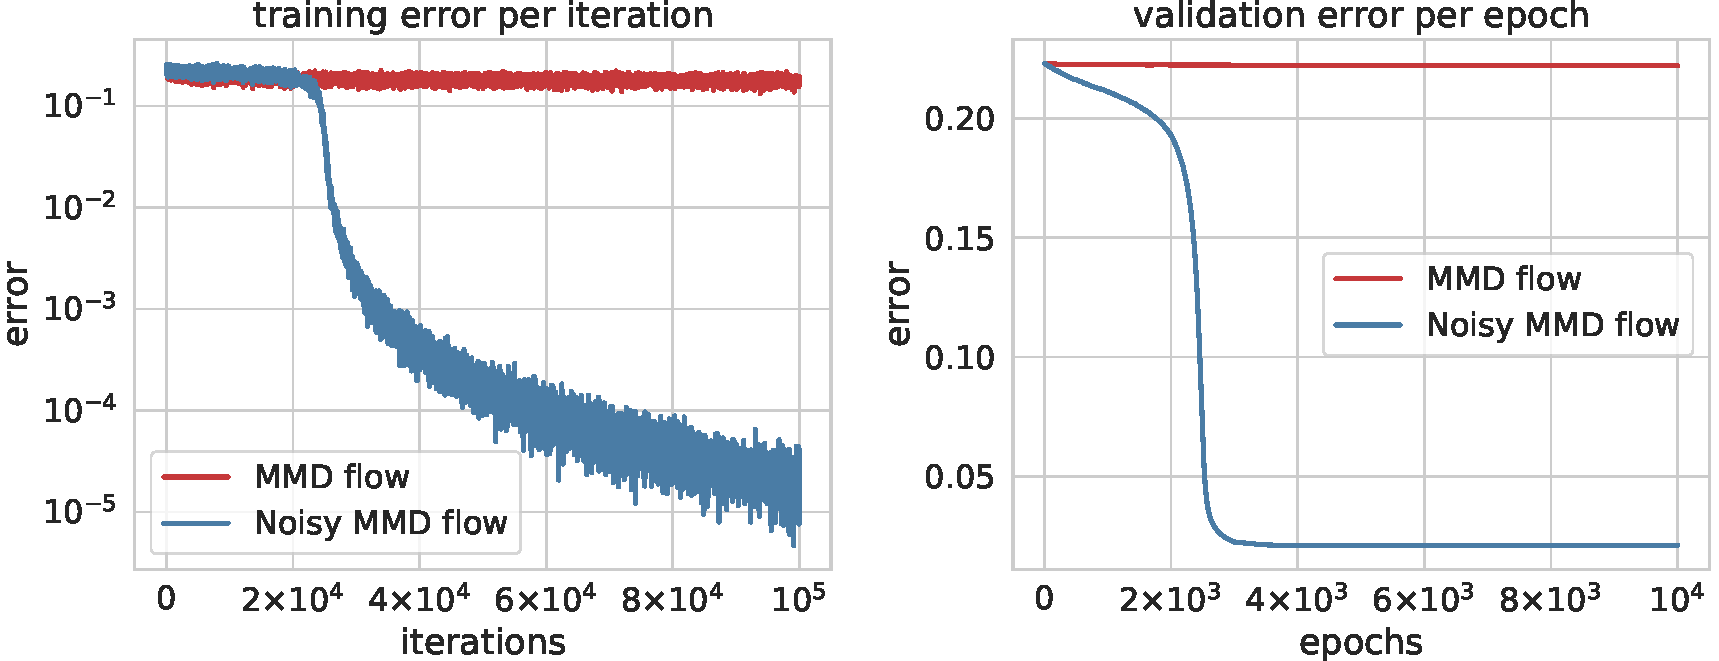
\includegraphics[width=0.8\linewidth]{figures/student_teacher_final}
	\caption{Gradient flow of the $MMD$ for training a student-teacher ReLU network with a gaussian output non-linearity. \cref{eq:euler_maruyama} is used without noise $\beta_n=0$ in red  and with noise $\beta_n>0$ in blue, with $\beta_0=1$ and $\beta_n$ is decreased by half after every $1000$ epochs. Training is done for $10^5$ epochs with a batch size of $10^2$ using $10^3$ samples and a step-size $\gamma = 0.01$. Details for the student-teacher setting are provided in \cref{sec:experiments}.   
	}
	\label{fig:experiments_student_teacher}
\end{figure}

\cref{fig:experiments_student_teacher} illustrates the behavior of the proposed algorithm \cref{eq:euler_maruyama} in a simple setting and compares it with the gradient flow of the MMD without noise injection. In this setting, a student network is trained to produce the outputs of a teacher network using gradient descent. As discussed in \cref{subsec:training_neural_networks} such setting can be seen as a particle version of an MMD flow with a suitable kernel. More details on the experiment are provided in \cref{sec:experiments}. Here, the MMD flow  fails to converge towards the global optimum and both training and validation error remain at value of $0.177$. On the other hand, adding noise to the gradient seems to lead to global convergence in terms of training error. The training error decreases below $10^{-5}$ while the validation error reaches $0.021$. It is worth noting that adding noise to the gradient slows the speed of convergence at the beginning of training. Such behavior is expected since the algorithm doesn't follow the path of steepest descent. The noise helps in escaping local optima, however, as illustrated here.


We consider an student-teacher network setting similar to \cite{Chizat:2018a}. More precisely, $f(\Theta,z)$  is a neural network of the form: $f((\theta_1,...\theta_N),z) = \frac{1}{N} \sum_{i=1}^N g(\theta_i,z) $ where $\Theta= (\theta_1,...,\theta_N)$ are the parameters and $z$ is the input vector in $\R^{p}$.  Each parameter $\theta_i$ is viewed as a particle so that the network $f$ is as an average of $N$ sub-networks $g$ with parameters $\theta_i$ where $g$ is given by:
\begin{align}
	g(\theta,z) = h(b^{1}+W^{1}\sigma(W^{0}z+b^{0})).
\end{align}
Here, $\theta = (b^{1},W^{1},b^{0},W^{0}) \in \R^1\times \R^{H}\times \R^{H} \times (\R^{H}\times\R^{p})$ and $\sigma$ is the ReLU non-linearity while $h$ is a fixed function and is defined later.
The teacher network $f_{T}(\Theta_T,z)$ has only one particle $N=1$ which is drawn  according to a normal distribution $\mathcal{N}(0,1.)$, while the student network $f_{S}(\Theta,z)$ has $N=1000$ particles that are initialized according to a normal distribution $\mathcal{N}(0.001,1.)$.  The inputs are drawn from a uniform distribution $\mathbb{S}$ on the sphere in $\R^p$ as in \cite{Chizat:2018a} with $p=50$. The number of hidden layers $H$ is set to $3$ and the output dimension is $1$.   
The parameters $\Theta$ of the student networks are trained to minimize the risk:
\begin{align}\label{eq:student_teacher_problem}
	\min_{\Theta} \mathbb{E}_{z\sim \mathbb{S} }[(f_T(\Theta_T,z )- f_S(\Theta,z))^2]
\end{align}
using SGD with mini-batches of size $100$ and a fixed step-size $\gamma=0.01$.

When $h$ is simply the identity function and no bias is used, one recovers the setting in \cite{Chizat:2018a}. In that case the network is partially $1$-homogeneous and \cite[Theorem 3.5]{Chizat:2018a} applies ensuring global optimality. Here, we are interested in the case when global optimality is not guaranteed by the homogeneity structure, hence we choose $h$ to be a gaussian with fixed bandwidth $\sigma=2.$. 
As shown in \cref{subsec:training_neural_networks}, performing gradient descent to minimize \cref{eq:student_teacher_problem} can be seen as a particle version of the $MMD$ flow with a kernel given by  $k(\theta,\theta') = \mathbb{E}_{z\sim\mathbb{S}}[g(\theta,z)g(\theta',z)] $. Hence one can use \cref{eq:euler_maruyama} to train the parameters of the student network. 

\cref{fig:experiments_student_teacher} illustrates the behavior of the proposed algorithm \cref{eq:euler_maruyama} in a simple setting and compares it with the gradient flow of the MMD without noise injection. In this setting, a student network is trained to produce the outputs of a teacher network using gradient descent. As discussed in \cref{subsec:training_neural_networks} such setting can be seen as a particle version of an MMD flow with a suitable kernel. More details on the experiment are provided in \cref{sec:experiments}. Here, the MMD flow  fails to converge towards the global optimum and both training and validation error remain at value of $0.177$. On the other hand, adding noise to the gradient seems to lead to global convergence in terms of training error. The training error decreases below $10^{-5}$ while the validation error reaches $0.021$. It is worth noting that adding noise to the gradient slows the speed of convergence at the beginning of training. Such behavior is expected since the algorithm doesn't follow the path of steepest descent. The noise helps in escaping local optima, however, as illustrated here.





\begin{figure}[ht]
	\centering
	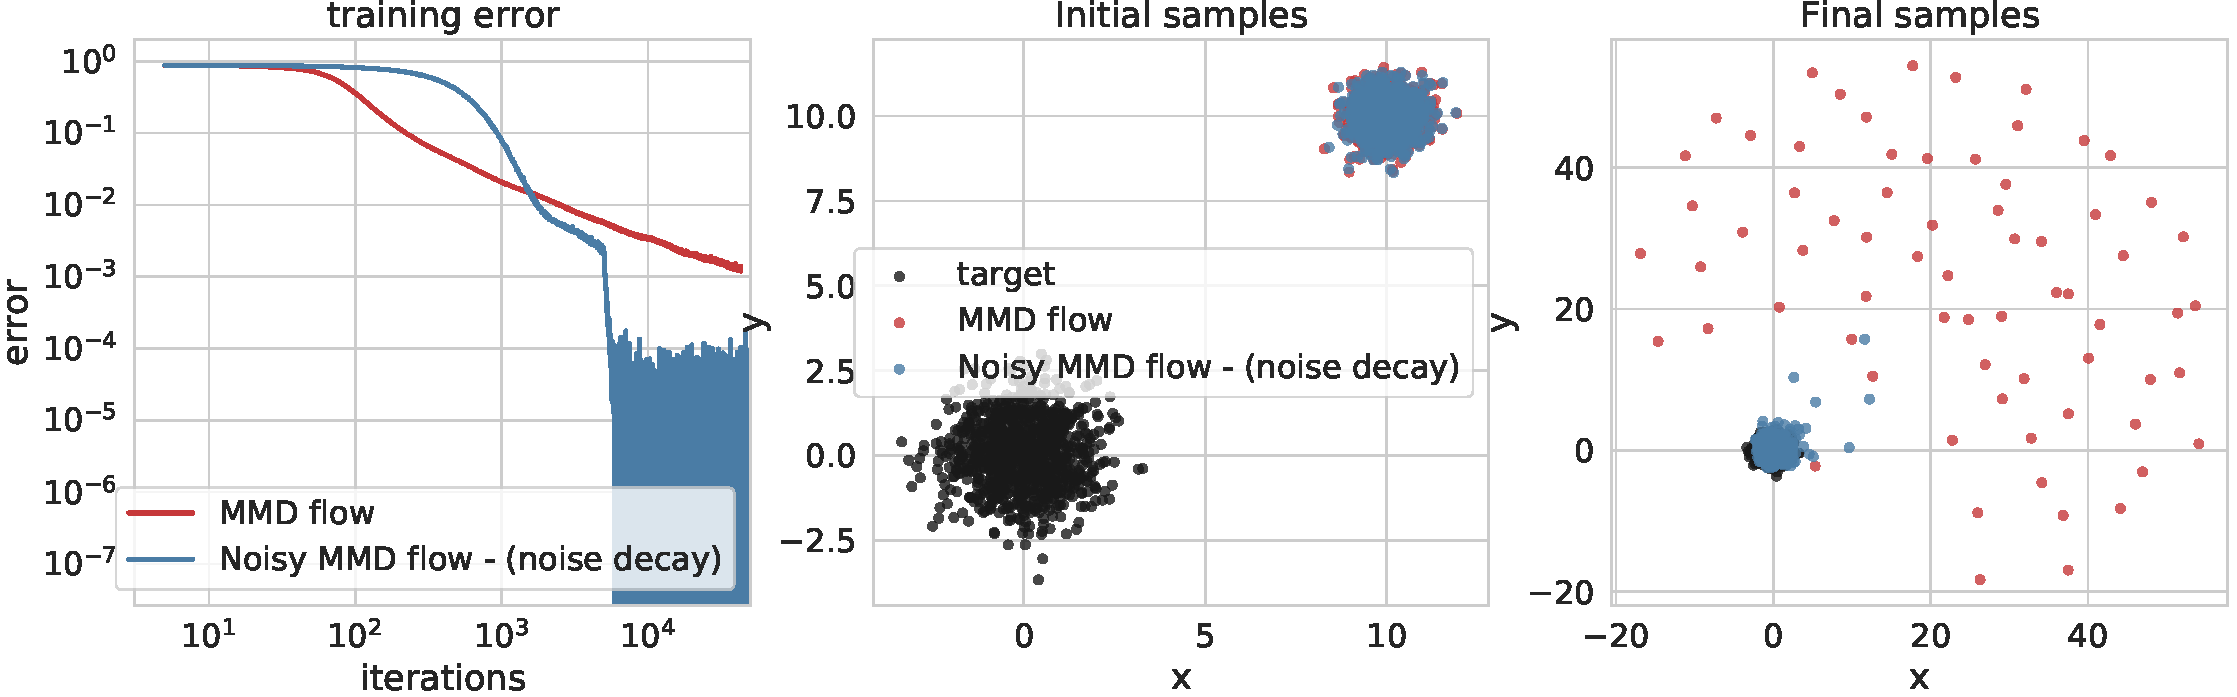
\includegraphics[width=0.8\linewidth]{figures/Gaussians_error_4}
	\caption{Gradient flow of the $MMD$ from a gaussian initial distributions $\nu_0\sim \mathcal{N}(10,0.5)$  towards a target distribution $\mu\sim \mathcal{N}(0,1)$ using $N=M=1000$ samples from $\mu$ and $\nu_0$ and a gaussian kernel with bandwidth $\sigma = 2 $. \cref{eq:euler_maruyama} is used 
	%with noise  $\beta_k = 10$ in blue, 
	without noise $\beta_n = 0$ in red and  with noise $\beta_n = 10$ up to $n=5000$, then $\beta_n = 0$ afterwards in blue. 
	The left figure shows the evolution of the $MMD$ at each iteration. The middle figure shows the initial samples (black for $\mu$), and the right figure shows the final samples after $10^5$ iterations with step-size $\gamma = 0.1$.}
	\label{fig:experiments}
\end{figure}
\cref{fig:experiments} illustrates the behavior of the proposed algorithm \cref{eq:euler_maruyama} in a simple setting, and compares it with the gradient flow of the MMD without noise injection. In this setting, the MMD flow  fails to converge to the global optimum. Indeed, as shown in \cref{fig:experiments}(right), some of the final samples (in red) obtained using noise-free gradient updates tend to get further away from the target samples (in black). Most of the remaining samples collapse to a unique point at the center near the origin. This can also be seen from \cref{fig:experiments}(left) where the training error fails to decrease below $10^{-3}$. On the other hand, adding noise to the gradient seems to lead to global convergence, as seen visually from the samples. The training error decreases below $10^{-4}$ and oscillates between $10^{-8}$ and $10^{-4}$. The oscillation is due to the step-size, which remained fixed while the noise was set to $0$ starting from iteration $5000$. It is worth noting that adding noise to the gradient slows the speed of convergence, as one can see from \cref{fig:experiments}(left). This is expected since the algorithm doesn't follow the path of steepest descent. The noise helps in escaping local optima, however, as  illustrated here.




\section{Auxiliary results}\label{sec:auxiliary_results}

\begin{proposition}\label{prop:grad_witness_function}
Under \cref{assump:lipschitz_gradient_k}, the witness function $f_{\mu,\nu}$ between any probability distributions $\mu$ and $\nu$ in $\mathcal{P}_2(\X)$ is differentiable and satisfies:
\begin{equation}\label{eq:gradient_witness}
\nabla f_{\mu,\nu}(z) = \int \nabla_1 k(z,x)\diff \mu(x) - \int \nabla_1 k(z,x)\diff \nu(x) \qquad \forall z\in \X
\end{equation}
where $z \mapsto \nabla_1 k(x,z)$ denotes the gradient of $z\mapsto k(x,z)$ for a fixed $x \in \X$.
 Moreover, the map $(z,\mu,\nu)\mapsto f_{\mu,\nu}(z)$ is Lipschitz with:
\begin{equation}\label{eq:lipschitz_grad_witness}
\Vert \nabla f_{\mu,\nu}(z) - \nabla f_{\mu',\nu'}(z')\Vert \leq 2L (\Vert z-z' \Vert + W_2(\mu,\mu') + W_2(\nu,\nu')) 
\end{equation}
Finally, each component of $\nabla f_{\mu,\nu}$ belongs to $\kH$.
\end{proposition}
\begin{proof}
	The expression of the witness function is given in \eqref{eq:witness_function}. To establish \eqref{eq:gradient_witness}, we simply need to apply the differentiation lemma \cite[Theorem 6.28]{Klenke:2008}. By \cref{assump:lipschitz_gradient_k}, it follows that $ (x,z)\mapsto \nabla_1 k(z,x)$ has at most a linear growth. Hence on any bounded neighborhood of $z$, $x\mapsto \Vert \nabla_1 k(z,x) \Vert $ is upper-bounded by an integrable function w.r.t. $\mu$ and $\nu$. Therefore, the differentiation lemma applies and  $\nabla f_{\mu,\nu}(z)$ is differentiable with gradient given by \cref{eq:gradient_witness}.
	
	To prove the second statement, we will consider two optimal couplings: $\pi_1$ with marginals $\mu$ and $\mu'$ and $\pi_2$ with marginals $\nu$ and $\nu'$.  We use \cref{eq:gradient_witness} to write:
	\begin{align*}
		\Vert \nabla f_{\mu,\nu}(z) - \nabla f_{\mu',\nu'}(z')\Vert 
		&= \Vert \mathbb{E}_{\pi_1}[ \nabla_1 k(z,x)-\nabla_1 k(z',x') ] - \mathbb{E}_{\pi_2}[\nabla_1 k(z,y)-\nabla_1 k(z',y')] \Vert\\
		& \leq
		\mathbb{E}_{\pi_1}[ \Vert  \nabla_1 k(z,x)-\nabla_1 k(z',x') \Vert ] + \mathbb{E}_{\pi_2}[\Vert  \nabla_1 k(z,y)-\nabla_1 k(z',y') \Vert ] \\
		&\leq
		L\left( \Vert  z-z' \Vert + \mathbb{E}_{\pi_1}[\Vert  x-x' \Vert]  +  \Vert  z-z' \Vert + \mathbb{E}_{\pi_2}[\Vert  y-y' \Vert ] \right)\\
		&\leq L(2\Vert z-z'\Vert + W_2(\mu,\mu')  + W_2(\nu,\nu') )
	\end{align*}
	The second line is obtained by convexity while the third one uses \cref{assump:lipschitz_gradient_k} and finally the last line relies on $\pi_1$ and $\pi_2$ being optimal. The desired bound is obtained by further upper-bounding the last two terms by twice their amount.
	%if we can pass the gradient inside the integral. It appears we can since the kernel verifies the following assumptions.
\end{proof}

%\begin{lemma}\label{lem:derivative_mmd}\manote{Notations still needs to be adjusted in this lemma}
%	Let $\phi$ be a vector field on $\X$ and $\nu$ in $\mathcal{P}_2(\X)$. Consider the path $\delta_t$ between $\nu$ and $(I+\phi)_{\#}\nu$ given by:
%	\begin{align*}
%		\delta_t=  (I+t\phi)_{\#}\nu \qquad \forall t\in [0,1]
%	\end{align*}
%The time derivative of $\mathcal{F}(\delta_t)$ is given by:
%	\begin{align*}
%		\dot{\F}(\delta_t)&=\int \nabla f_{\mu,\delta_t}(x+t\phi(x)) \phi(x)d\nu(x)\\
%	\end{align*}
%where $f_{\mu,\delta_t}$ is the witness function between $\mu$ and $\delta_t$ as defined in \cref{eq:witness_function}.	
%	Moreover, under \cref{assump:bounded_trace,assump:bounded_hessian}, the second time derivative satisfies:
%	\begin{align*}
%		\ddot{\F}(\delta_t) \vert \leq 3L \int \Vert \phi(x) \Vert^2 d\nu(x)
%	\end{align*}
%	where $L$ is a positive constant defined in \cref{assump:bounded_trace,assump:bounded_hessian}.
%	
%\end{lemma}
%\begin{proof}
%For simplicity, we write $f_t$ instead of $f_{\mu,\delta_t}$.
%We start by computing the first derivative. Recalling that $\mathcal{F}(\delta_t)$ is given by $\frac{1}{2}\Vert f_t\Vert^2_{\kH} $, it follows that:
%\[
%\dot{\F}(\delta_t)=\langle f_{t},\frac{df_{t}}{dt}\rangle_{\kH}.
%\]
%Using the definition
%of $\delta_{t}=(I+t\phi)_{\#}\nu$ we can write:\aknote{$\pi_t$? guess this corresponds to the paragraph below}
%\[
%\frac{df_{t}}{dt}=\int \phi(X).\nabla k(\pi_{t}(X),.)d\nu(X),
%\]
%hence:
%\[
%\frac{d\mathcal{F}(\delta_{t})}{dt}=2\int\phi(X).\nabla f_{t}(\pi_{t}(X))d\nu(X)
%\]
%Now the second derivative is obtained by direct derivation of the above expression:
%	\begin{align*}
%		\frac{d^2 \mathcal{F}(\delta_t)}{dt^2} =& \int \phi(X)^THf_t(\pi_t(X))\phi(X)d\nu(X)\\ 
%		&+\int \phi(X)^T\nabla_x\nabla_y k(\pi_t(X),\pi_t(X')) ) \phi(X')d\nu(X)d\nu(X') 
%	\end{align*}
%where $Hf_t$ is the hessian of $f_t$ in space and  $\nabla_x\nabla_y k(x,y)$ is the cross diagonal term of the hessian of $k$. By \cref{assump:bounded_hessian}, the first term in the above equation can be easily upper-bounded by:
%\begin{align*}
%	4L \int \Vert \phi(X)\Vert^2d\nu(X)  
%\end{align*}
%The last term can also be upper-bounded by $2L$ by \cref{assump:bounded_trace}.
%\end{proof}



\begin{lemma}\label{lem:derivative_mmd_augmented}
Let $U$ be an open set, $q$ a probability distribution in $\mathcal{P}_2(\X \times \mathcal{U})$ and $\psi$ and $\phi$ two measurable maps from  $\X \times\mathcal{U} $ to $\X$  which are square-integrable w.r.t $q$. Consider the path $\rho_t$ from  $(\psi)_{\#}q$ and $(\psi+\phi)_{\#}q$ given by: $\rho_t=  (\psi+t\phi)_{\#}q \quad \forall t\in [0,1]$. Under \cref{assump:lipschitz_gradient_k}, $\mathcal{F}(\rho_t)$ is differentiable in $t$ with
	\begin{align*}
		\dot{\F}(\rho_t)&=\int \nabla f_{\mu,\rho_t}(\psi(x,u)+t\phi(x,u)) \phi(x,u)\diff q(x,u)
	\end{align*}
where $f_{\mu,\rho_t}$ is the witness function between $\mu$ and $\rho_t$ as defined in \cref{eq:witness_function}.	
Moreover:
\begin{align*}
		\vert \dot{\F}(\rho_t) - \dot{\F}(\rho_s) \vert \leq 3L\vert t-s \vert\int \Vert \phi(x,u) \Vert^2 dq(x,u)
\end{align*}
\end{lemma}
\begin{proof}
For simplicity, we write $f_t$ instead of $f_{\mu,\rho_t}$ and denote by $s_t(x,u)= \psi(x,u)+t\phi(x,u)$
The function $h: t\mapsto k(s_t(x,u),s_t(x',u')) - k(s_t(x,u),z) - k(s_t(x',u'),z)$ is differentiable for all $(x,u)$,$(x',u')$ in $\X\times \mathcal{U}$ and $z\in \X$. 
Moreover, by \cref{assump:lipschitz_gradient_k}, a simple computation shows that for all $0\leq t\leq 1$:%\aknote{I would add the computation}
\[
\vert \dot{h} \vert \leq L\left[ (\Vert z - \phi(x,u)\Vert + \Vert \psi(x,u)\Vert) \Vert \phi(x',u')\Vert +  
(\Vert z - \phi(x',u')\Vert + \Vert \psi(x',u')\Vert )\Vert \phi(x,u)\Vert \right]
\]
The right hand side of the above inequality is integrable when $z$,  $(x,u)$ and  $(x',u')$ are independent and such that $z\sim \mu$ and both $(x,u)$ and $(x',u')$ are distributed according to $q$. Therefore, by the differentiation lemma \cite[Theorem 6.28]{Klenke:2008} it follows that $\F(\rho_t)$ is differentiable and:
\begin{align}\label{eq:time_derivative_mmd}
\dot{\F}(\rho_t) = \mathbb{E}\left[(\nabla_1 k(s_t(x,u),s_t(x',u'))-\nabla_1 k(s_t(x,u),z)).\phi(x,u)\right].
\end{align}
By \cref{prop:grad_witness_function}, we directly get $\dot{\F}(\rho_t) = \int \nabla f_{\mu,\rho_t}(\psi(x,u)+t\phi(x,u)) \phi(x,u)\diff q(x,u)$.
 We shall control now the difference $\vert \dot{F}(\rho_t)-\dot{\F}(\rho_{t'})\vert$ for $0\leq t,t'\leq 1$. Using \cref{assump:lipschitz_gradient_k} and recalling that $s_t(x,u)-s_{t'}(x,u)= (t-t')\phi(x,u)$ a simple computation shows:
\begin{align*}
	\vert\dot{\F}(\rho_t)-\dot{\F}(\rho_{t'}) \vert 
	&\leq L\vert t-t' \vert \mathbb{E}\left[(2\Vert \phi(x,u) \Vert + \Vert \phi(x',u')\Vert )\Vert \phi(x,u)\Vert  \right]\\
	  &\leq L\vert t-t'\vert(2\mathbb{E}\left[\Vert \phi(x,u)\Vert^2 \right]  + \mathbb{E}\left[\Vert \phi(x,u)\Vert \right]^2)\\
	 &\leq 3L\vert t-t'\vert\int\Vert \phi(x,u)\Vert^2 \diff q(x,u).
\end{align*}
which gives the desired upper-bound.
\end{proof}


\begin{lemma}\label{lem:second_derivative_augmented_mmd}
Let $q$ be a probability distribution in $\mathcal{P}_2(\X \times \X)$ and $\psi$ and $\phi$ two measurable maps from  $\X \times\X $ to $\X$  which are square-integrable w.r.t $q$. Consider the path $\rho_t$ from  $(\psi)_{\#}q$ and $(\psi+\phi)_{\#}q$ given by: $\rho_t=  (\psi+t\phi)_{\#}q \quad \forall t\in [0,1]$. Under \cref{assump:diff_kernel,assump:lipschitz_gradient_k}, $\mathcal{F}(\rho_t)$ is twice differentiable in $t$ with
	\begin{align*}
		\ddot{\F}(\rho_t)=&\mathbb{E}\left[\phi(x,y)^T\nabla_1 \nabla_2 k(s_t(x,y),s_t(x',y')) \phi(x',y')\right] \\
		&+ \mathbb{E}\left[\phi(x,y)^T (H_1k(s_t(x,y),y_t')-H_1k(s_t(x,y),z)) \phi(x,y)\right]
	\end{align*}
where $(x,y)$ and $(x',y')$ are independent samples from $q$, $z$ is a sample from $\mu$ and  $s_t(x,y)= \psi(x,y)+t\phi(x,y)$.
Moreover, if \cref{assump:bounded_fourth_oder} also holds then:
\begin{align*}
		\ddot{\F}(\rho_t) \geq \mathbb{E}\left[\phi(x,y)^T\nabla_1 \nabla_2 k(s_t(x,y),s_t(x',y')) \phi(x',y')\right] - \sqrt{2}\lambda d \F(\rho_t)^{\frac{1}{2}}\mathbb{E}[\Vert \phi(x,y) \Vert^2]  
\end{align*}
where we recall that $\X\subset \mathbb{R}^d$.
\end{lemma}
\begin{proof}
The first part is similar to \cref{lem:derivative_mmd_augmented}. In fact we already know by \cref{lem:derivative_mmd_augmented} that $\dot{\F}(\rho_t)$ exists and is given by:
\[
\dot{\F}(\rho_t) = \mathbb{E}\left[(\nabla_1 k(s_t(x,y),s_t(x',y'))-\nabla_1 k(s_t(x,y),z)).\phi(x,y)\right]
\]
Define now the function $\xi : t\mapsto (\nabla_1 k(s_t(x,y),s_t(x',y'))-\nabla_1 k(s_t(x,y),z)).\phi(x,y)$ which is differentiable for all $(x,y)$,$(x',y')$ in $\X\times \X$ and $z\in \X$ by \cref{assump:diff_kernel}. Moreover, its time derivative is given by:
\begin{align}
	\dot{\xi} =& \phi(x',y')^T \nabla_2\nabla_1k(s_t(x,y),s_t(x',y'))\phi(x,y) \\
	&+ \phi(x,y)^T(H_1k(s_t(x,y),s_t(x',y') ) - H_1k(s_t(x,y),z ))\phi(x,y)  
\end{align}
where $H_1 k$ denotes the Hessian of $k$. By \cref{assump:lipschitz_gradient_k} it follows in particular that $\nabla_2\nabla_1k$ and $H_1k$ are bounded hence $\vert \dot{\xi} \vert$  is upper-bounded by $ (\Vert \phi(x,y) \Vert + \Vert\phi(x',u') \Vert)\Vert \phi(x,y)\Vert$ which is integrable.
Therefore, by the differentiation lemma \cite[Theorem 6.28]{Klenke:2008} it follows that $\dot{\F}(\rho_t)$ is differentiable and $\ddot{\F}(\rho_t) = \mathbb{E}\left[\dot{\xi}\right].$
We prove now the second statement. Bu the reproducing property, it is easy to see that the last term in the expression of $\dot{\xi}$ can be written as:
\[
\langle \phi(x,y)^TH_1 k(s_t(x,y),.)\phi(x,y), k(s_t(x',y'),.)-  k(z,.)\rangle_{\kH} 
\]
Now, taking the expectation w.r.t $x'$  ,$y'$ and $z$ which can be exchanged with the inner-product in $\kH$ since  $(x',y',z)\mapsto k(s_t(x',y'),.)-  k(z,.)$ is Bochner integrable \cite[Definition 1, Theorem 6]{Retherford:1978} and recalling that such integral is given by $f_{\mu,\rho_t}$  one gets the following expression:
\[
 \langle  \phi(x,y)^TH_1 k(s_t(x,y),.)\phi(x,y), f_{\mu,\rho_t} \rangle_{\kH}
\]
Using Cauchy-Schwartz and \cref{assump:bounded_fourth_oder} it follows that:
\[
\vert \langle  \phi(x,y)^TH_1 k(s_t(x,y),.)\phi(x,y), f_{\mu,\rho_t} \rangle_{\kH}\vert \leq \lambda d\Vert \phi(x,y)\Vert^2 \Vert f_{\mu,\rho_t}\Vert 
\]
One then concludes using the expression of $\ddot{\F}(\rho_t)$ and recalling that $\F(\rho_t) = \frac{1}{2}\Vert f_{\mu,\rho_t} \Vert^2$.
\end{proof}

\begin{lemma}\label{lem:integral_lambda_convexity}
Assume that for any geodesic $(\rho_{t})_{t\in[0,1]}$ between
$\rho_{0}$ and $\rho_{1}$ in $\mathcal{P}(\X)$ with velocity vectors $(v_t)_{t \in [0,1]}$ the following holds:
\[
\ddot{\F}(\rho_{t}) \geq \Lambda(\rho_t,v_t)
\]
for some admissible functional $\Lambda$ as defined in \cref{def:conditions_lambda}, then:
\begin{align*}
\F(\rho_{t})\leq(1-t)\F(\rho_{0})+t\F(\rho_{1})-\int_{0}^{1}\Lambda(\rho_{s},v_{s})G(s,t)ds
\end{align*}
with $G(s,t)=s(1-t) \mathbbm{1}\{s\leq t\}
+t(1-s) \mathbbm{1}\{s\geq t\}$ for $0\leq s,t\leq 1$.

\end{lemma}
\begin{proof}
	This is a direct consequence of the general identity (\cite{Villani:2009},
	Proposition 16.2). Indeed, for any continuous function $\phi$ on
	$[0,1]$ with second derivative $\ddot{\phi}$ that is bounded below
	in distribution sense the following identity holds:
	\[
	\phi(t)=(1-t)\phi(0)+t\phi(1)-\int_{0}^{1}\ddot{\phi}(s)G(s,t)ds.
	\]
	This holds a fortiori for $\F(\rho_{t})$ since $\F$ is smooth. By assumption, we have that $\ddot{\F}(\rho_{t}) \geq \Lambda(\rho_t,V_t)$, hence, it follows that:
	\[
	\F(\rho_{t})\leq(1-t)\F(\rho_{0})+t\F(\rho_{1})-\int_{0}^{1}\Lambda(\rho_{s},v_{s})G(s,t)ds.
	\]
\end{proof}


\begin{lemma}\label{lem:mixture_convexity}[Mixture convexity]
	The functional $\F$ is mixture convex: for any probability distributions $\nu_1$ and $\nu_2$ and scalar $1\leq \lambda\leq 1$:
	\begin{align*}
	\F(\lambda \nu_1+(1-\lambda)\nu_2)\leq \lambda \F(\nu_1)+ (1-\lambda)\F(\nu_2)
	\end{align*}
\end{lemma}
\begin{proof}
	Let $\nu$ and $\nu'$ be two probability distributions and $0\leq \lambda\leq 1$. Expanding the RKHS norm in $\F$ it follows directly that:
	\[
		\mathcal{F}(\lambda \nu + (1-\lambda)\nu') -\lambda \mathcal{F}(\nu) -(1-\lambda)\mathcal{F}(\nu') = -\frac{1}{2}\lambda(1-\lambda)MMD(\nu,\nu')^2 \leq 0.
	\]
	which concludes the proof.
\end{proof}


%\begin{lemma}\label{lem:mmd_w2}[Lipschitzness of the MMD w.r.t. the $W_1$ and $W_2$ distance]
%	 Suppose that $k$ is bounded and measurable on $\X$, and that there exists $L_k$ such that $\forall x,y \in \X$, $\| k(x,.)-k(y,.) \|_{\kH}\le L_k \|x-y\|$. Then for all $\mu, \nu$ in $\mathcal{P}(\X)$:
%	\begin{equation}
%	MMD^2(\mu,\nu)\le  L_k^2 W_1^2(\mu,\nu) \le L_k^2 W_2^2(\mu,\nu)
%	\end{equation}
%\end{lemma}
%\begin{proof}
%Let $\mu, \nu$ in $\mathcal{P}(\X)$. By Proposition 20 in \cite{sriperumbudur2010hilbert} we have:
%\begin{equation}
%	MMD(\mu, \nu)	 \le \inf_{\pi \in \Pi(\mu, \nu)} \int \| k(x,.)-k(y,.) \|_{\kH} d\pi(\mu, \nu)
%\end{equation}
%Hence:
%\begin{align}
%	MMD^2(\mu, \nu)	
%	 \le (\inf_{\pi \in \Pi(\mu, \nu)} \int L_k \| x-y \| d\pi(\mu, \nu))^2
% \le L_k^2 W_1^2(\mu, \nu) \le L_k^2 W_2^2(\mu,\nu)
%\end{align}
%\end{proof}


\begin{lemma}
\label{lem:Discrete-Gronwall-lemma}[Discrete Gronwall lemma]
Let $a_{n+1}\leq(1+\gamma A)a_{n}+b$ with $\gamma>0$, $A>0$,
$b>0$ and $a_0=0$, then: 
\[
a_{n}\leq\frac{b}{\gamma A}(e^{n\gamma A}-1).
\]
\end{lemma}
\begin{proof}
	Using the recursion, it is easy to see that for any $n>0$:
	\[
	a_n \leq (1+\gamma A)^n a_0 + b(\sum_{i=0}^{n-1}(1+\gamma A )^{k}) 
	\]
	One concludes using the identity $\sum_{i=0}^{n-1}(1+\gamma A )^{k} =\frac{1}{\gamma A}((1+\gamma A)^{n} -1)$ and recalling that $(1+\gamma A)^{n} \leq e^{n\gamma A}$.
\end{proof}


%\subsection{Proof of \cref{prop:mmd_flow}}
%
%We firstly derive the strong subdifferential of $\F$ associated with the 2-Wasserstein metric. Since $\F= \frac{1}{2} \|f_t\|^2_{\kH}$, by simple derivations we obtain:
%\begin{equation}
% \nabla \frac{\partial\frac{1}{2} \|f_t\|^2_{\kH}}{\partial \rho_t}= \nabla \langle \frac{\partial f_t}{\partial \rho_t}, f_t \rangle_{\kH}= \nabla \langle \frac{\partial \E_{\rho_t}[k(Y,.)]}{\partial \rho_t}, f_t \rangle_{\kH}= \nabla \langle k(Y,.), f_t \rangle_{\kH}
%\end{equation}
%Then, by applying the reproducing property we have that:
%\begin{equation}
%\nabla \langle k(Y,.), f_t \rangle_{\kH}
%= \nabla f_t(Y)
%\end{equation}
%where $\nabla f_t(Y)= \E_{X \sim \rho_t}[\nabla_{Y}k(X,Y)] -  \E_{X \sim \pi}[\nabla_{Y}k(X,Y)]$.


%\begin{lemma}\label{lem:time_derivative}
%The time derivative of $\mathcal{F}(\rho_t)$ is given by:
%	\begin{align*}
%		\frac{d \mathcal{F}(\rho_t)}{dt}&=\int \nabla f_t(\pi_t(X)).(Y-X)d\Pi(X,Y)\\
%	\end{align*}
%	where $f_t$ is the witness function at time $t$ and is given by:
%	\begin{align}
%	f_t(x)=\rho_t(k(X,x))-\mu(k(X,x)) \qquad \forall t\in [0,1]
%	\end{align}	
%\end{lemma}
%\begin{proof}
%	The proof is very similar to the one in \cref{lem:derivative_mmd}. Indeed we still have
%	\begin{align*}
%		\frac{d \mathcal{F}(\rho_t)}{dt} = \langle f_t , \frac{df_t}{dt} \rangle
%	\end{align*}
%	And the time derivative of $f_t$ at each point $x\in\mathbb{R}^d$ is obtained by direct computation:
%	\begin{align*}
%		 \frac{df_t}{dt}= \int \nabla k(\pi_t(X,Y),.).(Y-X)d\Pi(X,Y)
%	\end{align*}
%	The result follows using the reproducing property in $\kH$.
% \end{proof}




%

\subsection{Additional mathematical background}

\subsubsection{MMD in Reproducing Kernel Hilbert Spaces (RKHS)}\label{sec:rkhs}

We recall here fundamental definitions and properties of reproducing kernel Hilbert spaces (RKHS) (see \cite{smola1998learning}) and Maximum Mean Discrepancies (MMD). The key aspect of a RKHS is
the reproducing property: for all $f \in \kH, f(x) = \langle f, k(x, .)\rangle_{\kH}$. 
Suppose that $k(.,.))$ is measurable and that $\E_x[k(x,x)]<\infty$.
Given $\mathcal{P}(\X)$ the set of probability measures defined on $\X$, $k$
is said to be characteristic if:
\begin{equation}
\mu \mapsto \int k(.,x) d\mu(x)
\end{equation}
is injective, i.e. $\mu$ is mapped to a unique element in $\kH$ called its mean embedding.  Suppose additionally that $k(.,.)$ is continuous, $\X$ is compact, and that $\kH$ is dense in $C(\X)$ the space of continuous bounded functions on $\X$. Under these conditions, the MMD is a metric (\cite{gretton2012kernel}, Theorem 5).



\subsubsection{Stochastic processes}\label{sec:ito_stochastic}

Consider the Itô process, i.e. the stochastic process:
\begin{equation}
dX_t=g(X_t)dt.
\end{equation}
Let $f$ be a twice-differentiable scalar function, Itô's formula (see \cite{ito1951stochastic}) can be written:
\begin{equation}
df(X_t)=\nabla f(X_t).g(X_t)dt
\end{equation}
Let $\rho_t$ be the distribution of the process $X_t$. We have:
\begin{align}
\E[\frac{df}{dt}(X_t)]&= \E[\nabla f(X_t).g(X_t)]\\
\Longleftrightarrow \int f(X) \frac{d \rho_t}{dt}(X)&=-\int f(X)div(g(X)\rho_t(X))
\end{align}
where the second line is obtained by integrating by parts on both sides of the equality. Finally, the distribution $\rho_t$ verifies the continuity equation: 
\begin{equation}
\frac{d\rho_t}{dt}=div(g\rho_t)
\end{equation}


\subsubsection{Additional lemmas}

\begin{lemma}\label{lem:mixture_convexity}
	The functional $\F$ is mixture convex: for any probability distributions $\nu_1$ and $\nu_2$ and scalar $1\leq \lambda\leq 1$:
	\begin{align*}
	\F(\lambda \nu_1+(1-\lambda)\nu_2)\leq \lambda \F(\nu_1)+ (1-\lambda)\F(\nu_2)
	\end{align*}
\end{lemma}
\begin{proof}
	Let $\nu$ and $\nu'$ be two probability distributions and $0\leq \lambda\leq 1$.
	We need to show that \[\mathcal{F}(\lambda \nu + (1-\lambda)\nu') -\lambda \mathcal{F}(\nu) -(1-\lambda)\mathcal{F}(\nu')\leq 0\]
	This follows from a simple computation which shows that:
	\begin{align*}
	\mathcal{F}(\lambda \nu + (1-\lambda)\nu') -\lambda \mathcal{F}(\nu) -(1-\lambda)\mathcal{F}(\nu') = -\frac{1}{2}\lambda(1-\lambda)MMD(\nu,\nu')^2 \leq 0.
	\end{align*}
\end{proof}


\begin{lemma}\label{lem:mmd_w2}
	 Suppose that $k$ is bounded and measurable on $\X$, and that there exists $L_k$ such that $\forall x,y \in \X$, $\| k(x,.)-k(y,.) \|_{\kH}\le L_k \|x-y\|$. Then for all $\mu, \nu$ in $\mathcal{P}(\X)$:
	\begin{equation}
	MMD^2(\mu,\nu)\le  L_k W_1^2(\mu,\nu) \le L_k W_2^2(\mu,\nu)
	\end{equation}
\end{lemma}
\begin{proof}
Let $\mu, \nu$ in $\mathcal{P}(\X)$. By Proposition 20 in \cite{sriperumbudur2010hilbert} we have:
\begin{equation}
	MMD(\mu, \nu)	 \le \inf_{\pi \in \Pi(\mu, \nu)} \int \| k(x,.)-k(y,.) \|_{\kH} d\pi(\mu, \nu)
\end{equation}
Hence:
\begin{align}
	MMD^2(\mu, \nu)	
	 \le (\inf_{\pi \in \Pi(\mu, \nu)} \int L_k \| x-y \| d\pi(\mu, \nu))^2
 \le L_k^2 W_1^2(\mu, \nu) \le L_k^2 W_2^2(\mu,\nu)
\end{align}
\end{proof}


%\subsection{Proofs of \cref{sec:mmd_flow}}

\subsubsection{Proof of \cref{prop:mmd_flow}}

In the case where $\F= \frac{1}{2} \|f_t\|^2_{\kH}$, by simple derivations we obtain:
\begin{equation}
 \nabla \frac{\partial\frac{1}{2} \|f_t\|^2_{\kH}}{\partial \rho_t}= \nabla \langle \frac{\partial f_t}{\partial \rho_t}, f_t \rangle_{\kH}= \nabla \langle \frac{\partial \E_{\rho_t}[k(Y,.)]}{\partial \rho_t}, f_t \rangle_{\kH}= \nabla \langle k(Y,.), f_t \rangle_{\kH}
\end{equation}
Then, by applying the reproducing property we have that:
\begin{equation}
\nabla \langle k(Y,.), f_t \rangle_{\kH}
= \nabla f_t(Y)
\end{equation}
where $\nabla f_t(Y)= \E_{X \sim \rho_t}[\nabla_{Y}k(X,Y)] -  \E_{X \sim \pi}[\nabla_{Y}k(X,Y)]$.

\subsubsection{Proof of \cref{prop:lambda_convexity} (Displacement convexity)}

We will firstly need the following lemma.

\begin{lemma}\label{lem:derivatives_witness}
	Let  $\mu$, $\nu_0$ and $\nu_1$ be three distributions in $\mathcal{P}_2(\X)$ and consider a displacement geodesic $(\rho_t)_{t\in[0,1]}$ between $\nu_0$ and $\nu_1$  defined by \cref{eq:displacement_geodesic} 
	and its corresponding velocity vector $(v_t)_{t\in [0,1]}$ as defined in \cref{eq:continuity_equation}. The following statements hold:
	\begin{enumerate}
		\item The first and second time derivatives of the witness function $f_{\mu,\rho_t}$ between $\mu$ and $\rho_t$ are well defined elements in $ \kH$ and are given by:
		\begin{align}\label{eq:derivatives_witness}
		\dot{f}_{\mu,\rho_t} = \int \nabla_1 k(x,.).v_t(x) \diff \rho_t(x); \qquad
		\ddot{f}_{\mu,\rho_t} = \int v_t(x)^T\nabla_1^2 k(x,.).v_t(x) \diff \rho_t(x)
		\end{align}
		where $ x \mapsto \nabla_1 k(x,z)$ and $x\mapsto \nabla_1^2 k(x,z)$ respectively denote the gradient and hessian of $x\mapsto k(x,z)$ for a fixed $z$ in $\X$.
		\item For all $g\in \kH$:
		\begin{align}\label{eq:inner_prod_deriative_witness}
		\langle g,\dot{f}_{\mu,\rho_t}\rangle_{\kH} = \int \nabla_1 g.v_t \diff \rho_t; \qquad
		\langle g,  \ddot{f}_{\mu,\rho_t}\rangle_{\kH} = \int v_t^T\nabla_1^2 g.v_t \diff \rho_t
		\end{align}
		\item The RKHS norms of $\dot{f}_{\mu,\rho_t}$ and $\ddot{f}_{\mu,\rho_t}$ satisfy:
		\begin{align}\label{eq:norm_derivative_witness}
		\Vert \dot{f}_{\mu,\rho_t}\Vert_{\kH}^2 = \langle v_t,C_{\rho_t} v_t \rangle_{L_2(\rho_t)}; \qquad  \Vert \ddot{f}_{\mu,\rho_t} \Vert\leq \lambda \Vert v_t \Vert^2_{L_2(\rho_t)}  
		\end{align}
		with $\lambda$ given by \cref{assump:bounded_fourth_oder} and $C_{\nu}$ defined in \cref{prop:lambda_convexity}. 
	\end{enumerate} 
\end{lemma}
\begin{proof}
	By definition of $\rho_{t}$:
	\[
	f_t(z)= \int k(x,z)\diff \mu(x) - \int k(s_t(x,y),z)\diff \pi(x,y)
	\]
	\manote{proof}
\end{proof}


\begin{proof}
To prove that $\nu\mapsto \F(\nu)$ is $\Lambda$-convex
we need to compute the second derivative $\ddot{\F}(\rho_{t})$
where $\rho_{t}$ is a displacement geodesic between two probability
distributions $\nu_{0}$ and $\nu_{1}$ as defined in \cref{eq:displacement_geodesic}. Such a minimizing geodesic always exists and can be written as $\rho_t = (s_t)_{\#}\pi$ with $s_t$ defined in \cref{eq:convex_combination} and $\pi$ is an optimal coupling between $\nu_0$ and $\nu_1$ (\cite{Santambrogio:2015}, Theorem 5.27). Moreover, we denote by $v_t$ the corresponding velocity vector as defined in \cref{eq:continuity_equation}. Recall from \cref{eq:mmd_norm_witness} that $\F(\rho_t) = \frac{1}{2} \Vert f_{\mu,\rho_t}\Vert^2_{\mathcal{H}}$, with $f_{\mu,\rho_t}$ defined in \cref{eq:witness_function}. To simplify notations we will write $f_t:= f_{\mu,\rho_t}$. We start by computing the first derivative of $ t\mapsto \F(\rho_t) $. By  \cref{lem:derivatives_witness},\cref{eq:derivatives_witness}, we know that $\dot{f}_t$ and $\ddot{f}_t $ are well defined elements of $\kH$ for any given $t\in [0,1]$, hence 
\[
 \dot{\F}(\rho_t) = \langle f_t, \dot{f_t}\rangle_{\kH};\qquad \ddot{\F}(\rho_t) = \Vert \dot{f_t}\Vert^2_{\kH} + \langle f_t, \ddot{f_t}\rangle_{\kH}.
 \]
While $\Vert \dot{f_t}\Vert^2_{\kH}$ is non-negative, $\langle f_t, \ddot{f_t}\rangle_{\kH}$ can in general be negative. We are only interested in quantifying how negative it can get, for this purpose we use Cauchy-Schwartz inequality which directly gives:
\[
\ddot{\F}(\rho_t)\geq  \Vert \dot{f}_t \Vert^2_{\kH} - \Vert f_t \Vert_{\kH}\Vert \ddot{f}_t\Vert_{\kH} 
\]

Finally by \cref{lem:derivatives_witness}, \cref{eq:norm_derivative_witness}, we can conclude that:
\[
	\ddot{\F}(\rho_t)\geq  \langle v_t,(C_{\rho_t} - \lambda \F(\rho_t)^{\frac{1}{2}}) v_t \rangle_{L_2(\rho_t)} 
\]
with $C_{\rho_t}$ given by \cref{eq:positive_operator_C} and $I$ is the identity operator in $L_2(\rho_t)$. Now we can introduce the function:
\begin{align}
	\Lambda(\nu,v) = \langle v ,( C_{\nu} -\lambda \F(\nu)^{\frac{1}{2}} I) v \rangle_{L_2(\nu)} 
\end{align}
which is defined for any pair $(\nu,v)$ with  $\nu\in \mathcal{P}_2(\X)$ and $v$ a square integrable vector field in $L_2(\nu)$. It is clear that $\Lambda(\nu,.)$  is a quadratic form on $L_2(\nu)$. Therefore, from \cref{def:lambda-convexity} of $\Lambda$ convexity, we conclude that $\F$ is $\Lambda$-convex.
\end{proof}


\subsubsection{Proof of \cref{cor:integral_lambda_convexity}}
\begin{proof}
	This is a direct consequence of the general identity (\cite{Villani:2009},
	Proposition 16.2). Indeed, for any continuous function $\phi$ on
	$[0,1]$ with second derivative $\ddot{\phi}$ that is bounded below
	in distribution sense the following identity holds:
	\[
	\phi(t)=(1-t)\phi(0)+t\phi(1)-\int_{0}^{1}\ddot{\phi}(s)G(s,t)ds
	\]
	Hence, one can choose $\phi(t)=\F(\rho_{t})$ therefore, \aknote{do we have second derivative bounded below for mmd?}
	it follows that:
	\[
	\F(\rho_{t})=(1-t)\F(\rho_{0})+t\F(\rho_{1})-\int_{0}^{1}\frac{d^{2}\F(\rho_{s})}{ds^{2}}G(s,t)ds
	\]
	Now using the inequality from \cref{prop:lambda_convexity}, \cref{eq:integral_lambda_convexity}
	follows directly. 
\end{proof}


\subsubsection{Proof of \cref{cor:loser_bound}}


\begin{proof}
	Recall the expression of $\Lambda(\rho_{s},v_{s}):$
	
	\[
	\Lambda(\rho_{s},v_{s})=\langle v_{t},(C_{\rho_{t}}-\lambda \F(\rho_{t})^\frac{1}{2} I)v_{t}\rangle_{L_{2}(\rho_{t})}\geq-\lambda \F(\rho_{t})^\frac{1}{2}\Vert v_{t}\Vert_{L_{2}(\rho_{t})}^{2}
	\]
	However, $\F(\rho_{t})^\frac{1}{2}\leq4C$ where $C=\sup_{x,y\in\mathcal{X}}\vert k(x,y)\vert$
	. Moreover, if $\rho_{t}$ is a constant speed geodesic then $\Vert v_{t}\Vert_{L_{2}(\rho_{t})}^{2}=W_{2}^{2}(\rho_{0},\rho_{1})$,
	hence: 
	\[
	-\int_{0}^{1}\Lambda(\rho_{s},v_{s})G(s,t)ds\leq\lambda 4CW_{2}^{2}(\rho_{0},\rho_{1})\int_{0}^{1}G(s,t)ds\leq2t(1-t)\lambda Cdiam(\mathcal{X})^{2}
	\]
	where $diam(\mathcal{X})$ is the diameter of $\mathcal{X}$. The rest of the proof follows by directly using \cref{cor:integral_lambda_convexity}
	and by setting $K=2\lambda Cdiam(\mathcal{X})$.
\end{proof}


\subsubsection{Proof of \cref{prop:almost_convex_optimization}}


\begin{proof}
	The proof is very similar to (\cite{Bottou:2017}, Theorem 6.3 and
	Theorem 6.9): \aknote{$\rho_1$ already taken}
	\begin{enumerate}
		\item First choose $\rho_{1}\in\mathcal{P}$ such that $\F(\rho_{1})<M-K$.
		For any $\rho_{0},\rho_{0}'\in L(\mathcal{P},M)$ there exist a displacement
		geodesic joining $\rho_{1}$ and $\rho_{0}$ without leaving $\mathcal{P}$,
		since $\mathcal{P}$ is by assumption discplacement convex. By \cref{cor:loser_bound}
		we have:
		\begin{align*}
		\F(\rho_{t}) & \leq(1-t)\F(\rho_{0})+t\F(\rho_{1})+t(1-t)K\\
		& \leq(1-t)M+t(M-K)+t(1-t)K\leq M-t^{2}K\leq M
		\end{align*}
		Hence $\rho_{t}\in L(\mathcal{P},M)$. The same can be done for a
		path joining $\rho_{0}'$ and $\rho_{1}$. Hence we can find a path
		in $L(\mathcal{P},M)$ joining $\rho_{0}$ and $\rho_{0}'$ , which
		means that the level set $L(\mathcal{P},M)$ is connected.
		\item Consider now $\rho_{1}\in L(\mathcal{P},M-K)$, note that such an
		element exists since $M>\inf_{\rho\in\mathcal{P}}\F(\rho)+K$.
		By convexity of $\mathcal{P}$ there exists a constant speed geodesic
		$\rho_{t}$ connecting $\rho_{0}$ and $\rho_{1}$. Since it is a
		constant speed curve then one has:
		\[
		W_{2}(\rho_{0},\rho_{t})\leq tW_{2}(\rho_{0},\rho_{1}).
		\]
		But we also have by \cref{cor:loser_bound}:
		\begin{align*}
		\F(\rho_{t}) & \leq(1-t)\F(\rho_{0})+t\F(\rho_{1})+t(1-t)K\\
		& \leq \F(\rho_{0})-t(\F(\rho_{0})-M+tK)\\
		& \leq \F(\rho_{0})-t(\F(\rho_{0})-M)
		\end{align*}
		Here we simply used the fact that $\rho_{1}\in L(\mathcal{P},M-K)$. 
	\end{enumerate}
\end{proof}
%


%
%
%
%By \cref{lem:derivatives_witness}, we have that $\dot{f_t}\in \kH$ and 
%
% it follows from \manote{some assumption to exchange orders}
%\[
%\frac{df_{t}}{dt}=\int(\nabla\phi(x)-x).\nabla k(\pi_{t}(x),.)\nu_{0}(x)dx
%\]
%hence:
%\[
%\frac{dMMD^{2}(\mu,\rho_{t})}{dt}=2\int(\nabla\phi(x)-x).\nabla f_{t}(\pi_{t}(x))\nu_{0}(x)dx
%\]
%Now the second derivative is given by:
%\begin{align*}
%\frac{d^{2}MMD^{2}(\mu,\rho_{t})}{dt^{2}}= & \int(\nabla\phi(x)-x).Hf_{t}(\pi_{t}(x))(\nabla\phi(x)-x)\nu_{0}(x)dx\\
% & +\int(\nabla\phi(x)-x).\nabla_{1}\nabla_{2}k(\pi_{t}(x),\pi_{t}(x'))(\nabla\phi(x')-x')\nu_{0}(x)\nu_{0}(x')dxdx'
%\end{align*}
%Here $\nabla_{1}\nabla_{2}k(x,x')$ is the matrix whose components
%are given by $\langle\partial_{i}k(x,.),\partial_{j}k(x,.)\rangle$
%for $1\leq i,j\leq d$, and $Hf_{t}$ is the hesssian of $f_{t}$
%and its components are also given by:
%\[
%(Hf_{t}(x))_{i,j}=\langle f_{t},\partial_{i}\partial_{j}k(x,.)\rangle.
%\]
%Denoting by $h(x):=\nabla\phi(x)-x$ it follows that:
%\begin{align*}
%\frac{d^{2}MMD^{2}(\mu,\rho_{t})}{dt^{2}}= & \langle f_{t},\int\sum_{i,j}h_{i}(x)h_{j}(x)\partial_{i}\partial_{j}k(\pi_{t}(x),.)\nu_{0}(x)dx\rangle\\
% & +\Vert\int\sum_{i}h_{i}(x)\partial_{i}k(\pi_{t}(x),.)\nu_{0}(x)dx\Vert^{2}
%\end{align*}
%Now we use Cauchy-Schwartz inequality for the first term to get:
%\begin{align*}
%\frac{d^{2}MMD^{2}(\mu,\rho_{t})}{dt^{2}}\geq & -\Vert f_{t}\Vert_{\kH}\Vert\int\sum_{i,j}h_{i}(x)h_{j}(x)\partial_{i}\partial_{j}k(\pi_{t}(x),.)\nu_{0}(x)dx\Vert_{\kH}\\
% & +\Vert\int\sum_{i}h_{i}(x)\partial_{i}k(\pi_{t}(x),.)\nu_{0}(x)dx\Vert^{2}.
%\end{align*}
%After applying a change of variables $x=\pi_{t}(y)$ one recovers the
%velocity vector $v_{t}$ instead of $h$: 
%\begin{align*}
%\frac{d^{2}MMD^{2}(\mu,\rho_{t})}{dt^{2}}\geq & -\Vert f_{t}\Vert_{\kH}\Vert\int\sum_{i,j}v_{t}^{i}(x)v_{t}^{j}(x)\partial_{i}\partial_{j}k(x,.)\rho_{t}(x)dx\Vert_{\kH}\\
% & +\Vert\int\sum_{i}v_{t}^{i}(x)\partial_{i}k(x,.)\rho_{t}(x)dx\Vert^{2}.
%\end{align*}
%
%One can further note that:
%\[
%\Vert\int\sum_{i,j}v_{t}^{i}(x)v_{t}^{j}(x)\partial_{i}\partial_{j}k(x,.)\rho_{t}(x)dx\Vert_{\kH}\leq\lambda\Vert v_{t}\Vert_{L_{2}(\rho_{t})}^{2}
%\]
%
%and that 
%\begin{align*}
%\Vert\int\sum_{i}v_{t}^{i}(x)\partial_{i}k(x,.)\rho_{t}(x)dx\Vert^{2} & =\int v_{t}(x)^{T}\int\nabla_{1}\nabla_{2}k(x,x')v_{t}(x')\rho_{t}(x')dx'dx.\\
% & =\langle v_{t},C_{\rho_{t}}v_{t}\rangle_{L_{2}(\rho_{t})}
%\end{align*}
%
%Hence we have shown that 
%\[
%\frac{d^{2}MMD^{2}(\mu,\rho_{t})}{dt^{2}}\geq\langle v_{t},(C_{\rho_{t}}-\lambda MMD(\mu,\rho_{t})I)v_{t}\rangle_{L_{2}(\rho_{t})}=\Lambda(\rho_{t},v_{t})
%\]

%
\subsection{Proofs of \cref{sec:discretized_flow}}

\subsubsection{Proof of \cref{prop:decreasing_functional}}

\begin{lemma}	\label{lem:grad_flow_lambda_version}
Let $\nu$ be a distribution in $\mathcal{P}_2(\X)$ and $\mu$ the target distribution such that $\F(\mu)=0$.  Let $\pi$ be an optimal coupling between $\nu$ and $\mu$, and $\rho_t$ the displacement geodesic defined by \cref{eq:displacement_geodesic} with its corresponding velocity vector  $v_t$ as defined in \cref{eq:continuity_equation}. Finally let $\phi(X)=\nabla f_{\nu,\mu}(X)$ the gradient of the witness function between $\mu$ and $\nu$. The following inequality holds: \manote{This should be a standard result, just need to cite it}
\begin{align*}
	\int \phi(x).(y-x) d\pi(x,y)
	\leq
	\F(\mu)- \F(\nu) -\int_0^1 \Lambda(\rho_s,v_s)(1-s)ds
\end{align*}

\end{lemma}
\begin{proof}
Recall that $\rho_t$ is given by $\rho_t = (s_t)_{\#}\pi$. By $\Lambda$-convexity of $\mathcal{F}$ the following inequality holds:
	\begin{align*}
		\mathcal{F}(\rho_{t})\leq (1-t)\mathcal{F}(\nu)+t \mathcal{F}(\mu) - \int_0^1 \Lambda(\rho_s,v_s)G(s,t)ds
	\end{align*}
	Hence by bringing $\mathcal{F}(\nu)$ to the l.h.s and dividing by $t$ and then taking its limit at $0$ it follows that:
	\begin{align*}
	\dot{\F}(\rho_t)\vert_{t=0}\leq \mathcal	{F}(\mu)-\mathcal{F}(\nu)-\int_0^1 \Lambda(\rho_s,v_s)(1-s)ds.	
	\end{align*}
	Moreover, by \cref{lem:derivatives_witness}, the time derivative of the witness function between $\nu$ and $\mu$ is well defined, so that $\dot{\F}(\rho_t)$ can be written as:
	\[
	\dot{\F}(\rho_t) = \langle f_{\mu,\rho_t},\dot{f}_{\mu,\rho_t} \rangle_{\kH}
	\]
	Now by \cref{lem:derivatives_witness},\cref{eq:inner_prod_deriative_witness} it follows that:
\[
\dot{\F}(\rho_t) = \int \nabla f_{\mu,\rho_t}(x).v_t(x)\diff \rho_t(x)
\]
By definition of $\rho_t$,  one can further write:
\[
\dot{\F}(\rho_t) = \int \nabla f_{\mu,\rho_t}(s_t(x,y)).(y-x)\diff \pi(x,y)
\]
where we used the fact that $v_t(s_t(x,y))=(y-x)$\manote{cite something}. Hence at $t=0$ we get:
\[
\dot{\F}(\rho_t)\vert_{t=0} = \int \nabla f_{\mu,\nu}(x).(y-x)\diff \pi(x,y)
\]
which shows the desired result.
\end{proof}





\begin{lemma}\label{lem:derivative_mmd}\manote{Notations still needs to be adjusted in this lemma}
	Let $\phi$ be a vector field on $\X$ and $\nu$ in $\mathcal{P}_2(\X)$. Consider the path $\delta_t$ between $\nu$ and $(I+\phi)_{\#}\nu$ given by:
	\begin{align*}
		\delta_t=  (I+t\phi)_{\#}\nu \qquad \forall t\in [0,1]
	\end{align*}
The time derivative of $\mathcal{F}(\delta_t)$ is given by:
	\begin{align*}
		\dot{\F}(\delta_t)&=\int \nabla f_{\mu,\delta_t}(x+t\phi(x)) \phi(x)d\nu(x)\\
	\end{align*}
where $f_{\mu,\delta_t}$ is the witness function between $\mu$ and $\delta_t$ as defined in \cref{eq:witness_function}.	
	Moreover, under \cref{assump:bounded_trace,assump:bounded_hessian}, the second time derivative satisfies:
	\begin{align*}
		\ddot{\F}(\delta_t) \vert \leq 3L \int \Vert \phi(x) \Vert^2 d\nu(x)
	\end{align*}
	where $L$ is a positive constant defined in \cref{assump:bounded_trace,assump:bounded_hessian}.
	
\end{lemma}
\begin{proof}
For simplicity, we write $f_t$ instead of $f_{\mu,\delta_t}$.
We start by computing the first derivative. Recalling that $\mathcal{F}(\delta_t)$ is given by $\frac{1}{2}\Vert f_t\Vert^2_{\kH} $, it follows that:
\[
\dot{\F}(\delta_t)=\langle f_{t},\frac{df_{t}}{dt}\rangle_{\kH}.
\]
Using the definition
of $\delta_{t}=(I+t\phi)_{\#}\nu$ we can write:\aknote{$\pi_t$? guess this corresponds to the paragraph below}
\[
\frac{df_{t}}{dt}=\int \phi(X).\nabla k(\pi_{t}(X),.)d\nu(X),
\]
hence:
\[
\frac{d\mathcal{F}(\delta_{t})}{dt}=2\int\phi(X).\nabla f_{t}(\pi_{t}(X))d\nu(X)
\]
Now the second derivative is obtained by direct derivation of the above expression:
	\begin{align*}
		\frac{d^2 \mathcal{F}(\delta_t)}{dt^2} =& \int \phi(X)^THf_t(\pi_t(X))\phi(X)d\nu(X)\\ 
		&+\int \phi(X)^T\nabla_x\nabla_y k(\pi_t(X),\pi_t(X')) ) \phi(X')d\nu(X)d\nu(X') 
	\end{align*}
where $Hf_t$ is the hessian of $f_t$ in space and  $\nabla_x\nabla_y k(x,y)$ is the cross diagonal term of the hessian of $k$. By \ref{assump:bounded_hessian}, the first term in the above equation can be easily upper-bounded by:
\begin{align*}
	4L \int \Vert \phi(X)\Vert^2d\nu(X)  
\end{align*}
The last term can also be upper-bounded by $2L$ by \ref{assump:bounded_trace}.
\end{proof}

Let $  \nu$ and $\nu'$ be two distributions and $\Pi$ a coupling between $\nu$ and $\nu'$. We consider the path $\rho_t$ defined as $\rho_t=(\pi_t)_{\#}\Pi$ where $\pi_t(X,Y)=(1-t)X+tY$. It is possible to provide an expression for the time derivative of $\mathcal{F}{\rho_t}$. This is given by ?\\\aknote{beware, not finished!}

%\begin{lemma}\label{lem:time_derivative}
%The time derivative of $\mathcal{F}(\rho_t)$ is given by:
%	\begin{align*}
%		\frac{d \mathcal{F}(\rho_t)}{dt}&=\int \nabla f_t(\pi_t(X)).(Y-X)d\Pi(X,Y)\\
%	\end{align*}
%	where $f_t$ is the witness function at time $t$ and is given by:
%	\begin{align}
%	f_t(x)=\rho_t(k(X,x))-\mu(k(X,x)) \qquad \forall t\in [0,1]
%	\end{align}	
%\end{lemma}
%\begin{proof}
%	The proof is very similar to the one in \cref{lem:derivative_mmd}. Indeed we still have
%	\begin{align*}
%		\frac{d \mathcal{F}(\rho_t)}{dt} = \langle f_t , \frac{df_t}{dt} \rangle
%	\end{align*}
%	And the time derivative of $f_t$ at each point $x\in\mathbb{R}^d$ is obtained by direct computation:
%	\begin{align*}
%		 \frac{df_t}{dt}= \int \nabla k(\pi_t(X,Y),.).(Y-X)d\Pi(X,Y)
%	\end{align*}
%	The result follows using the reproducing property in $\kH$.
% \end{proof}




\begin{proof}
	Here we consider a path between $\nu_n$ and $\nu_{n+1}$ of the form:
	\begin{align*}
	\rho_t	=(I-\gamma t\phi_n)_{\#}\nu_n
	\end{align*}
	The function $t\mapsto \mathcal{F}(\rho_t)$ is twice differentiable, hence one can use a Taylor expansion with integral remainder to get:
	\begin{align}\label{eq:taylor_expansion}
	\mathcal{F}(\nu_{n+1})-\mathcal{F}(\nu_{n})=\mathcal{F}(\rho_1)-\mathcal{F}(\rho_0) = \frac{d \mathcal{F}(\rho_t) }{dt}\vert_{t=0}+ \frac{1}{2} \int_0^1 \frac{d^2 \mathcal{F}(\rho_t)}{dt^2}(1-t)^2 dt 
	\end{align} 
	By taking $\phi=-\gamma \phi_n$ in \cref{lem:derivative_mmd} we have that:
	\begin{align*}
	\frac{d \mathcal{F}(\rho_t) }{dt} = -\gamma \int \nabla f_n(X).\phi_n(X)d\nu_n(X)=-\gamma \int \Vert \phi_n(X) \Vert^2 d\nu_n(X)
	\end{align*}
	since $\nabla f_n=\phi_n$.
	Moreover, by \cref{assump:bounded_trace,assump:bounded_hessian} it follows from \cref{lem:derivative_mmd} that:
	\begin{align}\label{eq:upper_bound_1}
	\vert \frac{d^2 \mathcal{F}(\rho_t) }{dt^2}   \vert\leq L\int \Vert \phi_n(X) \Vert^2 d\nu_n(X)
	\end{align}
	Using \cref{eq:taylor_expansion,eq:upper_bound_1} the result follows.
\end{proof}

\subsubsection{Proof of \cref{prop:evi}}

\begin{proof}
	Let $\Pi^n$ be the optimal coupling between $\nu_n$ and $\mu$, then the optimal transport between $\nu_n$ and $\mu$ is given by:
	\begin{align}
	W_2^2(\mu,\nu_n)=\int \Vert X-Y \Vert^2 d\Pi^n(\nu_n,\mu)
	\end{align}
	Moreover, consider $Z=X-\gamma \phi_n(X)$ where $(X,Y)$ are samples from $\Pi^n$. It is easy to see that $(Z,Y)$ is a coupling between $\nu_{n+1}$ and $\mu$, therefore, by definition of the optimal transport map between $\nu_{n+1}$ and $\mu$ it follows that:
	\begin{align}\label{eq:optimal_upper-bound}
	W_2^2(\nu_{n+1},\mu)\leq \int \Vert X-\gamma \phi_{n}(X)-Y\Vert^2 d\Pi^n(\nu_n,\mu)
	\end{align}
	By expanding the r.h.s in \cref{eq:optimal_upper-bound}, the following inequality holds:
	\begin{align}\label{eq:main_inequality}
	W_2^2(\nu_{n+1},\mu)\leq W_2^2(\nu_{n},\mu) -2\gamma \int \langle \phi_n(X), X-Y \rangle d\Pi^n(\nu_n,\mu)+ \gamma^2D(\nu_n)
	\end{align}
	where $D(\nu_n) = \int \Vert \phi_n(X)\vert^2 d\nu_n $.
	An upper-bound on $-2\gamma \int \langle \phi_n(X), X-Y \rangle d\Pi^n(\nu_n,\mu) $ in terms of the loss functional can be obtained using the $\Lambda$ displacement convexity of $\nu\mapsto \F(\nu)$. Indeed, by \cref{lem:grad_flow_lambda_version} it holds that:
	\begin{align}\label{eq:flow_upper-bound}
	-2\gamma \int  \phi(X).(X-Y) d\Pi(\nu,\mu)
	\leq
	-2\gamma\left(\F(\nu)- \F(\mu) +K(\rho^n)\right)
	\end{align}
	where $(\rho^n_t)_{0\leq t \leq 1}$ is a constant-speed geodesic from $\nu_n$ to $\mu$ and $K(\rho^n):=\int_0^1 \Lambda(\rho^n_s,\dot{\rho^n}_s)(1-s)ds$\aknote{as Adil said, we should try to quantify this}. Note that when $K(\rho^n)\leq 0$ it falls back to the convex setting.
	Therefore, the following inequality holds:
	\begin{align}
	W_2^2(\nu_{n+1},\mu)\leq W_2^2(\nu_{n},\mu) - 2\gamma\left(\F(\nu_n)- \F(\mu) +K(\rho^n)\right) +\gamma^2 D(\nu_n)
	\end{align}
	Now we introduce a term involving $\F(\nu_{n+1})$. The above inequality becomes:
	\begin{align}
	W_2^2(\nu_{n+1},\mu)\leq & W_2^2(\nu_{n},\mu) - 2\gamma\left(\F(\nu_{n+1})- \F(\mu) +K(\rho^n)\right) \\
	&+\gamma^2 D(\nu_n) -2\gamma (\F(\nu_n)-\F(\nu_{n+1}))
	\label{eq:main_ineq_2}
	\end{align}
	It is possible to upper-bound the last two terms by a negative quantity when the step-size is small enough. This is mainly a consequence of the smoothness of the functional $\F$ and the fact that $\nu_{n+1}$ is obtained by following the steepest direction of $\F$ starting from $\nu_n$. \cref{prop:decreasing_functional} makes this statement more precise and enables to get the following inequality:
	\begin{align}
	\gamma^2 D(\nu_n) -2\gamma (\F(\nu_n)-\F(\nu_{n+1})\leq -\gamma^2 (1-\gamma L)D(\nu_n),
	\label{eq:decreasing_functional}
	\end{align}
	where $L$ is a constant that depends only on the choice of the kernel $k$ in $\F$. Combining  \cref{eq:main_ineq_2} and \cref{eq:decreasing_functional} it follows that:
	\begin{align}
	2\gamma(\F(\nu_{n+1})-\F(\mu))+\gamma^2(1-\gamma L)D(\nu_n)
	\leq 
	W_2^2(\nu_n,\mu)-W_2^2(\nu_{n+1},\mu)-2\gamma K(\rho^n).
	\label{eq:main_final}
	\end{align}
\end{proof}

\subsubsection{Proof of \cref{th:rates_mmd}}



